% “华为杯”第二十三届中国研究生数学建模竞赛论文
% 使用 XeLaTeX 编译：latexmk -xelatex main.tex
% 封面必须保留；学校、参赛队号与队员姓名仅出现在封面，正文不得出现任何身份信息。
\documentclass[bwprint]{gmcmthesis}

% === 额外宏包（cls 未内置的）===
% 附件2 规定「正文引用处用方括号标示参考文献的编号，如[1][3]等」，故用行内方括号编号
% 而非上标（natbib 的 super 模式）。分隔符保持逗号：规范里的 [1][3] 是「引用两篇」的
% 示意写法，改成 ][ 会把引用串拉宽，收益不抵重排风险。
\setcitestyle{numbers,square,comma}
% 附录 A 的代码清单表有 23 行、实测高约 840pt，而本版式 \textheight 只有约 688pt
% （geometry top=30mm/bottom=25mm）——它装不进一页，必须允许跨页。xltabular 是
% longtable 与 tabularx 的合体（可断页 + X 列 + 表头跨页重复），且仍是非浮动表。
\usepackage{xltabular}
% cls 中 \thefigure 等取「节号.序号」，必须让计数器在每节/每附录处归零，否则出现 2.2、6.4 之类的跳号
\counterwithin*{figure}{section}
\counterwithin*{table}{section}
\counterwithin*{equation}{section}

% 长 \texttt 文件名（results/q1\_ilp\_gap.csv 之类）与数学串内部没有断行点，西文与 CJK
% 混排顶到行末时会直接顶出版心。emergencystretch 只在最后一遍断行生效，用来吸收这类
% 无法拆分的长 token，正常段落不受影响（本值不改变任何断行位置的取舍，只兜底）。
\setlength{\emergencystretch}{3em}

% === 竞赛信息（仅用于封面）===
\title{山区洪涝灾害下无人机运输与通信协同优化}
\baominghao{20260095597}
\schoolname{沈阳工业大学}
\membera{陆长顺}
\memberb{文学鹏}
\memberc{郭浩彬}

% ①②③④ 等「带圈字母数字」（U+2460 起）不在 Times New Roman 的 cmap 内，而 cls 用
% \setmainfont{Times New Roman} 作西文主字体；XeTeX 对缺失字形是静默丢弃——不报错、
% 但页面上就是空白，日志里只留一条 Missing character。把该区段并入 CJK 字符类后
% 改由 \CJKmainfont（本机即 SimSun）出字，正文的「配置 ④ ⊇ ③」才不会缺字。
\xeCJKDeclareCharClass{CJK}{"2460 -> "24FF}

% === 目录 ===
% 版式（黑体章条、宋体节条、点线引导、章前 7pt 间距）由 cls 的 tocloft/titletoc 设定，
% 这里只定层级与标题字样：列到「节」为止，标题用「目 录」与摘要页的「摘 要：」呼应。
\setcounter{tocdepth}{2}
\renewcommand{\contentsname}{目\quad 录}

% === 结果数字的统一来源（由 code/paper_metrics.py 生成，勿手改）===
% 该文件把每个结果数字定义成宏（\mtQoneEnergy 等），数值与出处见
% results/paper_metrics.json。正文用到这些数的地方一律写宏，脚本重跑一次即同步。
% 本文件由 code/paper_metrics.py 自动生成，请勿手工编辑。
% 每个宏的数值与出处见 results/paper_metrics.json。

\newcommand{\mtQfourAllPartitions}{364}
\newcommand{\mtQfourCV}{0.7462}
\newcommand{\mtQfourFeasible}{0}
\newcommand{\mtQfourGapSum}{2}
\newcommand{\mtQfourK}{2}
\newcommand{\mtQfourPartitions}{5}
\newcommand{\mtQfourR}{30}
\newcommand{\mtQfourRedundancy}{2}
\newcommand{\mtQfourRelayNeed}{3}
\newcommand{\mtQfourUnits}{7}
\newcommand{\mtQoneAreas}{15}
\newcommand{\mtQoneEnergy}{59.236}
\newcommand{\mtQoneIlpAgree}{14}
\newcommand{\mtQoneIlpCases}{15}
\newcommand{\mtQoneIlpGapCases}{45}
\newcommand{\mtQoneMass}{758.000}
\newcommand{\mtQoneMaxRound}{2370.6}
\newcommand{\mtQoneMinSoc}{22.83\%}
\newcommand{\mtQoneTrips}{18}
\newcommand{\mtQoneWorkTimeH}{9.10}
\newcommand{\mtQoneWorkTimeS}{32771.8}
\newcommand{\mtQthreeCoverageStep}{1.0}
\newcommand{\mtQthreeDelaySum}{11862.3}
\newcommand{\mtQthreeDirect}{66.18\%}
\newcommand{\mtQthreeGap}{0.00\%}
\newcommand{\mtQthreeIntervals}{21}
\newcommand{\mtQthreeJointDone}{10853.3}
\newcommand{\mtQthreeJointEnergy}{73.676}
\newcommand{\mtQthreeLateBoxes}{6}
\newcommand{\mtQthreeMaxLate}{5472.5}
\newcommand{\mtQthreeMinMargin}{69.3}
\newcommand{\mtQthreeRelayEnergy}{4.963}
\newcommand{\mtQthreeRelayFrac}{33.82\%}
\newcommand{\mtQthreeRelays}{6}
\newcommand{\mtQthreeSegs}{71}
\newcommand{\mtQthreeStaggered}{5}
\newcommand{\mtQthreeStations}{3}
\newcommand{\mtQthreeTardiness}{223301.0}
\newcommand{\mtQthreeTransDone}{10853.3}
\newcommand{\mtQthreeTransEnergy}{68.713}
\newcommand{\mtQtwoBoxes}{80}
\newcommand{\mtQtwoEnergy}{68.713}
\newcommand{\mtQtwoExactCases}{6}
\newcommand{\mtQtwoExactProved}{5}
\newcommand{\mtQtwoExactTimeout}{1}
\newcommand{\mtQtwoHardViol}{0}
\newcommand{\mtQtwoMakespan}{8732.6}
\newcommand{\mtQtwoParetoRows}{6}
\newcommand{\mtQtwoRecEnergy}{68.713}
\newcommand{\mtQtwoRecK}{20}
\newcommand{\mtQtwoRecMakespan}{8732.6}
\newcommand{\mtQtwoRecTrips}{20}
\newcommand{\mtQtwoScanRows}{6}
\newcommand{\mtQtwoSeed}{20260923}
\newcommand{\mtQtwoTardiness}{0.0}
\newcommand{\mtQtwoTrips}{20}
\newcommand{\mtQtwoUavs}{8}


\begin{document}

\maketitle

% === 摘要（恰一页：矛盾与主线 / 四问各一段 / 系统层结论 / 关键词）===
% 组织方式：第 1 段立「矛盾—主轴—主线」，第 2–5 段按「建了什么→得到什么关键结果→说明什么」，
% 第 6 段升到系统层。数字一律取自 sections/generated_metrics.tex 的 \mtXXX 宏或 results/ 实测值。
\begin{abstract}
	山区洪涝灾害救援受复杂地形、严格配送时限与通信遮挡的叠加约束：异构无人机在载荷、航程与能耗上差异显著，共享电池与中继能源组件需周转、可用运力随时钟变化。本文以应急时效为核心，把问题提炼为硬时限、能源周转与连续通信约束下的运输—通信—资源协同调度，先建立四问共享的地形感知飞行—能耗—通信统一模型，再沿“能力评估—时效调度—通信协同—资源配置”逐问求解。

	\textbf{对于问题一}，按 30\,m DEM 逐像元确定巡航海拔，结合载荷—航程等效与爬升附加能耗建立单点往返能力模型，二分求得各机型在各服务区的最大安全载荷，C 型在 S008 降至 58.57\,kg；再把机型并入架次模式，用多重集动态规划在\textbf{允许混用机型}的可行域上按字典序求得精确最优组批，得 \mtQoneTrips\ 架次、总能耗 \mtQoneEnergy\,kWh、累计作业时间 \mtQoneWorkTimeH\,h，较限定一区一型节能 $6.24\%$。灵敏度分析给出方案整体失效的临界返航安全余量 0.3513，且率先失效的是轻载 A 型而非重载 C 型。

	\textbf{对于问题二}，在医疗与首批物资硬时限、机队与电池库存、充电周转约束下，把货箱组批、服务区访问顺序、机型、执行无人机、共享电池、派工顺序与各架次开始时刻一并作为决策变量，以精确组批耦合大邻域自适应搜索、并用 $\varepsilon$-约束扫描架次数上限，得 \mtQtwoRecTrips\ 个运输架次、总能耗 \mtQtwoEnergy\,kWh、完成时间 \mtQtwoMakespan\,s，加权时延与硬时限违约均为 $0$。消融实验显示，仅优化派工顺序就使完成时间下降 $31.9\%$，表明调度结构本身是系统效率的重要来源。

	\textbf{对于问题三}，沿问题二方案的三维轨迹逐时刻判定直连链路，得直连时间占比 $\mtQthreeDirect$、盲区 $\mtQthreeRelayFrac$——运输层的高效方案在“连续通信、中断必须为 $0$”的硬约束下不可执行。本文把运输开始时刻与错峰、中继站址与离地高度、中继架次调度放入同一优化问题，以候选站网格配合集合覆盖整数规划分层最小化站数与中继能耗，得 \mtQthreeStations\ 个悬停站、\mtQthreeRelays\ 次出动共 \mtQthreeRelayVisits\ 次悬停站服务、中继能耗 \mtQthreeRelayEnergy\,kWh，在本文二值视线遮挡口径下中断占比由 $\mtQthreeRelayFrac$ 降至 $0$；代价是联合完工时刻由 \mtQtwoMakespan\,s 推迟至 \mtQthreeJointDone\,s，而迟到箱数与加权迟到仍为 $0$，表明连续通信可靠性与应急时效间存在明确权衡。

	\textbf{对于问题四}，按“同一架次的服务区不可拆分”把 15 个服务区绑定为 \mtQfourUnits\ 个原子任务单元，$K=2$ 与 $K=3$ 的 2047 与 $86\,526$ 种分区经完全枚举即得全局最优的资源核算。按题面“资源不得跨组调配”复核，两种分组的库存可行分区数均为 \mtQfourFeasible；枚举进一步厘清成因：八类资源各自的最小缺口在两 $K$ 下\textbf{全部为 $0$}，逐类看均有解，故不可行来自多类资源无法在同一分区内同时满足的\textbf{联合约束}，其中中继下界 $K-1$ 在 $K=3$ 时恰等于库存、余量为 $0$。推荐分区在 $K=2$ 缺 \mtQfourGapSum\ 件、$K=3$ 缺 \mtQfourMinPatchKThree\ 件，故给出补配清单而非可行分区。

	结果表明，山区无人机应急救援的瓶颈并非单一能耗，而是配送时限、异构运力、能源周转、地形遮挡与连续通信共同形成的时空资源冲突：单层运输最优并不等于系统可执行最优——本文的创新正在于把地形感知的飞行—能耗—通信统一模型与运输、通信、资源三层决策纳入同一优化框架，使联合调度成为可执行方案。

	\keywords{无人机应急运输；异构无人机调度；通信中继；地形感知；大邻域自适应搜索；协同调度；资源配置}
\end{abstract}

% === 目录（摘要在前、正文在后；abstract 环境自带 \clearpage，故目录起新页）===
% article 系的 \tableofcontents 不像 report 那样自带 \clearpage，
% 后面必须自己清页，否则正文第一章会接在目录最后一行下面。
\maketoc
\clearpage

\pagestyle{plain}

% === 正文 ===
\section{问题重述}
\subsection{问题背景}

山区洪涝灾害具有突发性强、影响范围分散以及道路、供电和通信设施同时受损等特点。连续强降雨引发的山洪、滑坡和道路塌方，会使部分居民点在短时间内与外界失去稳定的地面交通联系。灾后早期，饮用水、应急食品、医疗物资和生活卫生用品需要尽快送达，而传统车辆难以及时进入地形起伏大、道路受损严重的区域。无人机受地面道路条件影响较小，因而成为应急运输的重要补充手段。

2026 年 7 月，受台风“美莎克”带来的持续强降雨影响，广西横州市镇龙乡遭遇严重洪涝灾害，一度出现断路、断电、断网，全乡约 8000 人受困，救援人员与物资一度只能依靠空中投送进入受灾区域\cite{xinhua2026jizhe,xinhua2026sanji}。本题以镇龙乡及周边山区为地理背景，设置标准测试场景：1 个临时调度中心（O01）、15 个服务区（S001--S015）和 80 个不可拆货箱，配置三种运输无人机机型（A/B/C）共 8 架实体运输无人机、配套共享电池组、30\,m 数字高程模型（DEM）数据、中继无人机、可更换能源组件及无线链路参数。地理环境如图~\ref{fig:dem-map}所示。

\begin{figure}[htbp]
	\centering
	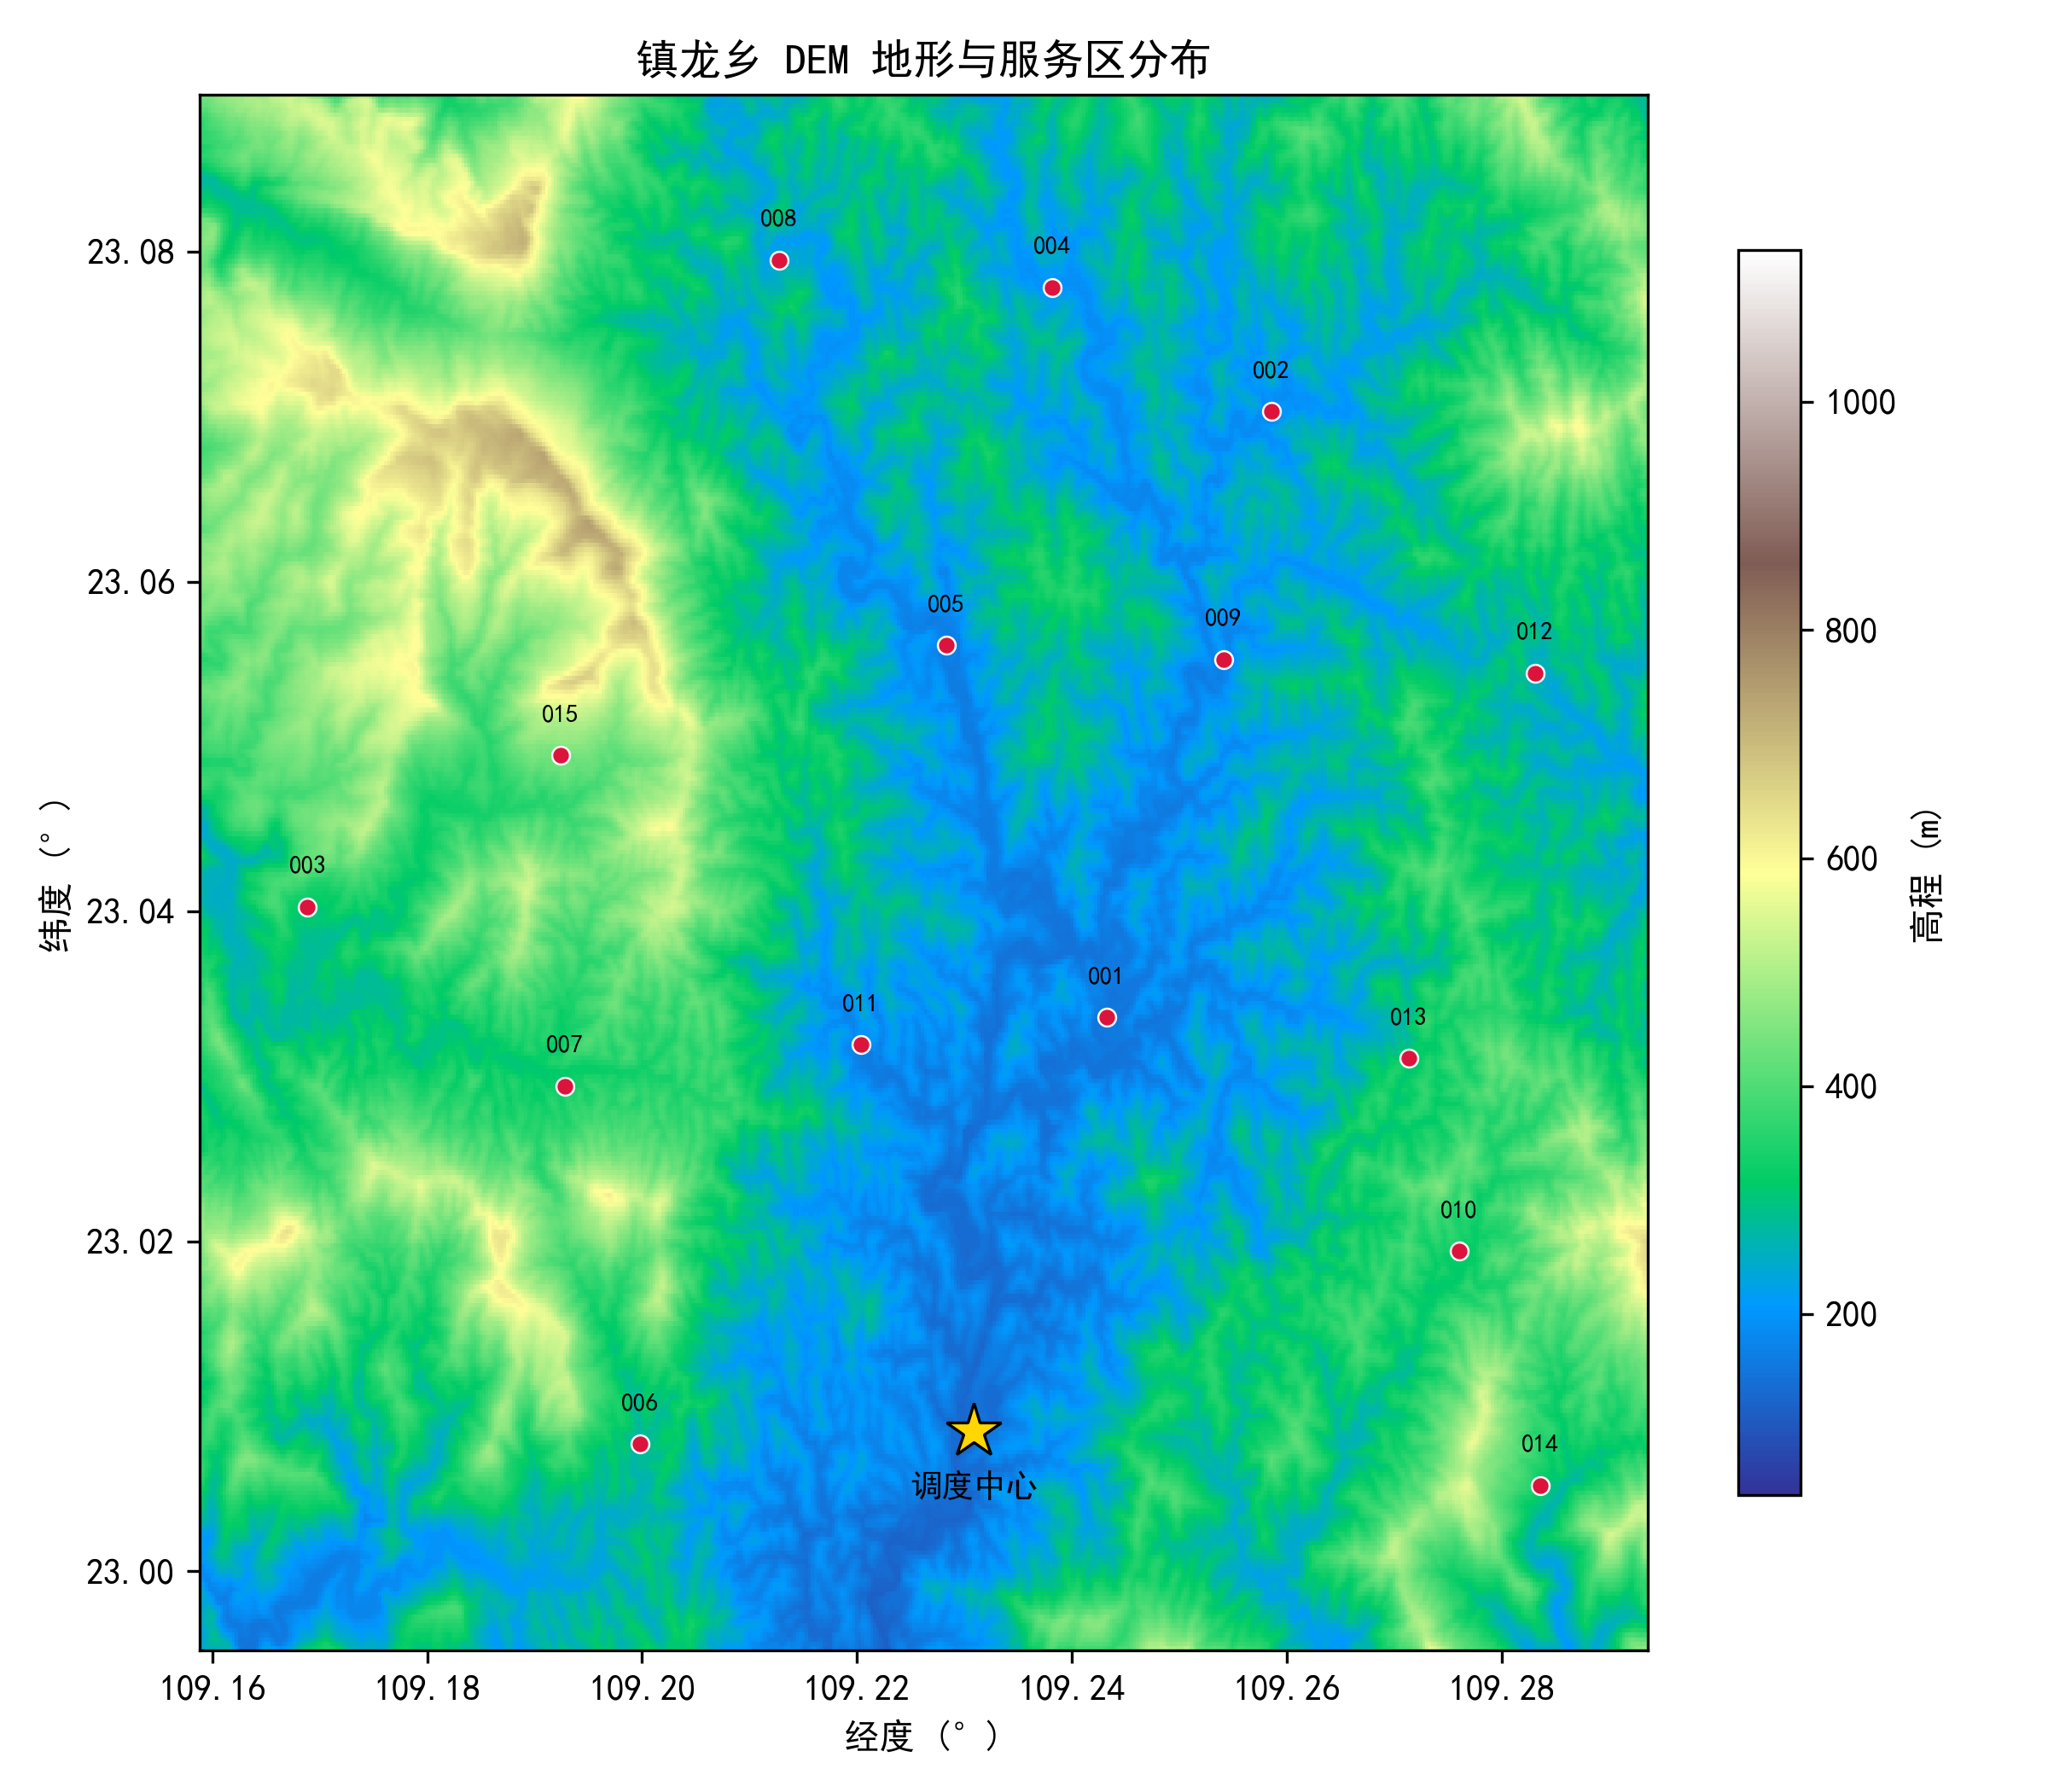
\includegraphics[width=0.82\textwidth]{figures/fig_dem_map.png}
	\caption{镇龙乡 DEM 地形与调度节点分布}
	\label{fig:dem-map}
\end{figure}

图~\ref{fig:dem-map}的地形分布直接决定了后文的三条建模口径。其一，\textbf{调度中心与多数服务区并不在同一个高度带上}：色标跨度约 $200\sim1000$\,m，中部有一条南北向的低海拔谷地，O01 正落在谷底，而 S002、S004、S008、S012 等点位于谷地两侧的较高处——故「同一段航程的两端高差」不能忽略，巡航海拔必须按航段沿线实际经过的地形抬升，而不是取两端点的较大值。其二，\textbf{高差是连续起伏而非台阶}：谷地与西侧、东北侧的高脊之间没有平坦过渡，同一航段会在数公里内跨越数百米的高差，这正是第 4 章把巡航海拔取为「沿线所过 DEM 像元的最高地面高程」而非两点插值的原因。其三，\textbf{谷地对两侧构成天然遮挡}：O01 处在低处，而服务区散布在谷地两侧与更远处，两端点之间的视线很容易被中途的脊线切断——这解释了为什么直连通信并非处处可用，也说明中继需求是地形本身带来的，而不是参数设置偏严所致。

\subsection{问题重述}

\noindent \textbf{问题 1（单点往返运输能力与货箱组批方案）：}在不考虑实体无人机和共享电池调度的前提下，研究单服务区直接往返（O01$\to$S$_i\to$O01）条件下的运输能力与货箱组批。要求计算三种机型在不同服务区的最大安全载荷；在货箱不可拆分且满足载质量、装载体积和返航安全能量余量的条件下确定各服务区货箱组批方案；综合考虑架次数、总能耗和累计作业时间对组批方案进行优化并说明指标权衡；并讨论返航安全余量变化对最大安全载荷和组批结果的影响。

\noindent \textbf{问题 2（异构无人机多点多架次运输调度）：}在不考虑通信保障的情况下，研究异构运输无人机的多点多架次调度。每个运输架次可访问一个或多个服务区并返回 O01，在货箱不可拆、载质量与体积、返航安全余量、无人机与共享电池数量、充电周转及物资时限等约束下，联合确定货箱组批、服务区访问顺序、机型、执行无人机、共享电池及各架次开始时刻，并优化配送及时性、任务完成时间、能耗和架次数。

\noindent \textbf{问题 3（通信约束下的运输与中继联合调度）：}在考虑通信保障的情况下，研究运输无人机与中继无人机的联合调度。运输无人机全程需保持连续通信，直连地面网关不可用时由空中中继无人机保障。要求联合确定运输与中继的组批、时序、机型及中继悬停位置、飞行海拔、服务时段和能源组件分配。

\noindent \textbf{问题 4（救援任务分区与资源配置优化）：}以问题三的联合调度方案为基础，将 15 个服务区划分为 2 个和 3 个任务组（保持已确定的组批、访问顺序、运输与中继安排及通信保障关系不变），分别核算各任务组独立执行所需的各类资源数量，并从资源规模、冗余、组间工作量均衡及与库存的缺口等方面比较两种分区方式。
      % 一、问题重述
\section{总体分析与总技术路线图}

\subsection{总体分析}

本题的核心是一个在复杂地形与通信约束下，运输无人机、中继无人机与能源资源多类要素的协同优化问题，四个子问题呈递进关系，公共物理规则、单位与对象编号保持一致。

\textbf{问题一}是能力评估与组批问题。每个架次为单服务区直接往返，故各服务区相互独立，问题可分解为“单点往返最大安全载荷计算”与“货箱装箱组批”两个层次。前者由地形净空（巡航海拔）、等效航程模型和爬升附加能耗共同决定，可用二分法精确求解；后者是典型的一维装箱（bin packing）问题\cite{martello1990knapsack}，货箱不可拆分且需同时满足质量、体积与能量余量约束。

\textbf{问题二}是带资源约束的多机型车辆路径问题（VRP）的推广\cite{dorling2017vehicle}。相比经典 VRP，其难点在于：载荷随投送过程递减使得航段能耗非线性；共享电池按机型分池且需两阶段充电周转；医疗与首批物资带硬时限。由于规模较大且约束耦合，采用“构造启发式＋离散事件调度”的两阶段求解策略，并用对比实验刻画指标间的权衡。

\textbf{问题三}在问题二的基础上叠加通信约束，是运输—中继联合调度问题。通信状态由视线遮挡（地形）与双向链路预算共同判定\cite{itu2024p525,zeng2016wireless}，需对运输无人机轨迹逐时刻采样判定直连/中继/中断三种状态；中继悬停位置与时段则构成一个带时间窗的几何覆盖问题，可用“候选点网格＋集合覆盖”求解。

\textbf{问题四}是任务分区与资源配置问题。在保持问题三调度关系不变的前提下，将服务区划分为若干任务组，本质是对“多服务区架次”所约束的服务区进行聚类，并在组间不可调配资源的条件下核算各组峰值资源需求，进而比较不同分区方式的资源规模、冗余与缺口。

四个问题间的数据继承关系为：问题一的组批能力与能耗模型为问题二提供基础；问题二的运输调度方案为问题三的通信分析提供运输轨迹与时段；问题三的联合调度方案为问题四的分区提供待划分的任务单元。据此，本文首先统一建立公共物理模型，再逐问递进求解：问题一给出的最大安全载荷与组批结论构成问题二装箱时的容量输入，问题二得到的运输架次及其时段是问题三逐时刻判定通信状态的直接对象，问题三的运输—中继联合调度方案又构成问题四划分任务组时的待绑定单元。上述路线汇总于下页的总体技术路线图。

% 参照竞赛优秀论文的通行画法：整页竖排、纯黑白、每条带对应一个子问题，
% 纵向五带（公共物理模型＋四问）× 横向四栏（阶段），节标题即图题。
% 三点务必保留：① 不加 \caption（否则白占一个图号，且与节标题重复）；
% ② 用 \clearpage + 非浮动排版的精确落版，改用 [p] 浮动体会被推迟若干页；
% ③ 宽度取 0.97\textwidth——按 0.97 计高 621pt，加节标题 40pt 后余量 27pt，
%    取满 \textwidth 则只剩 8pt 余量，字号或行距稍变即溢出到次页。
\clearpage
\subsection{总技术路线图}

\begin{center}
	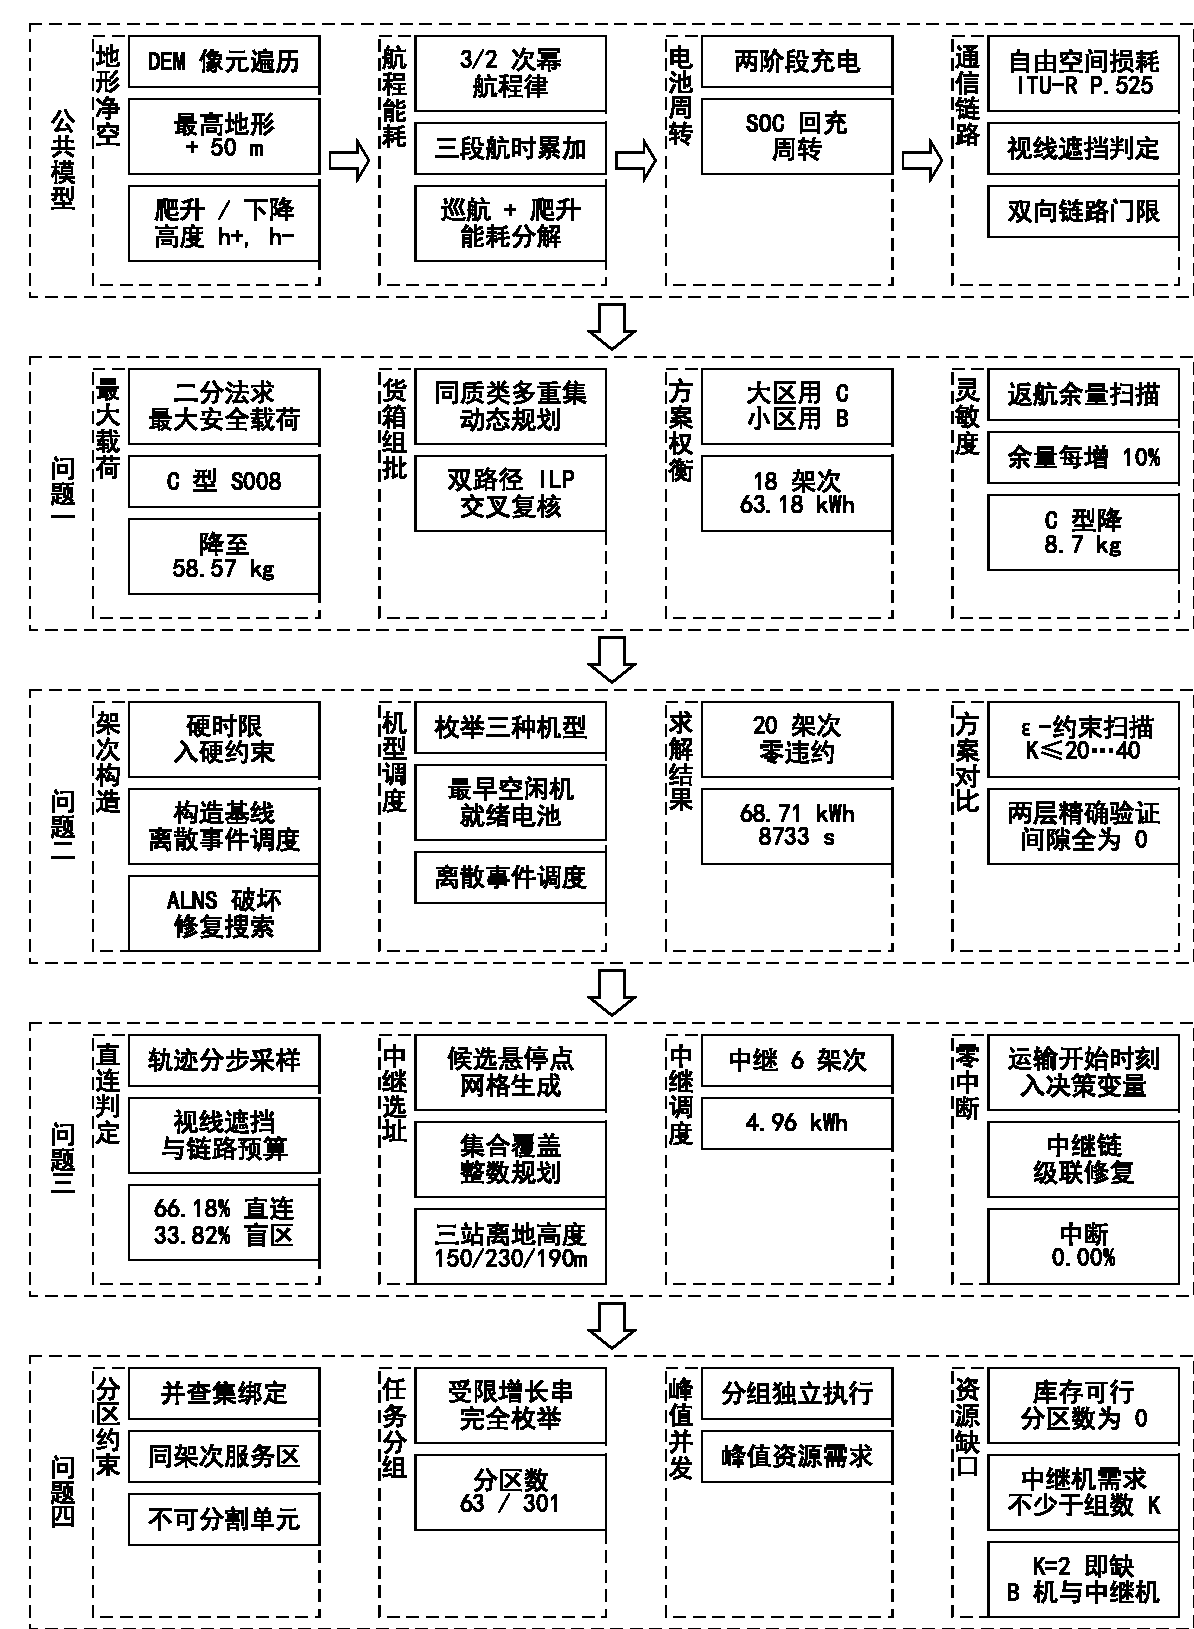
\includegraphics[width=0.97\textwidth]{figures/fig_roadmap.pdf}
\end{center}
          % 二、总体分析与总技术路线图
\section{模型假设与符号说明}

\subsection{模型假设}
为在保证问题本质不丢失的前提下建立可计算的模型，本文做出以下假设：
\begin{itemize}
	\item \textbf{假设 1（直线航段）：}任意两个任务节点之间采用两点间的水平直线作为运输航段，水平巡航距离按局部平面投影（WGS84）计算。
	\item \textbf{假设 2（巡航海拔）：}计划巡航海拔取该航段所经过 DEM 像元的最高地面高程以上 50\,m，且不低于起终点作业高度；爬升与下降为竖直运动，水平巡航为定高飞行。
	\item \textbf{假设 3（能耗口径）：}水平巡航能耗由等效航程反推（$E^{\mathrm{hor}}=E^{\mathrm{use}}\cdot d/L_g(q)$），爬升附加能耗取重力势能除以爬升能耗效率；下降不单独计能耗（效率为 0）。
	\item \textbf{假设 4（理想环境）：}忽略风、雨、能见度等气象因素对飞行时间与能耗的影响；无人机起降、悬停、交接过程稳定可靠。
	\item \textbf{假设 5（充电模型）：}电池与能源组件统一采用题给两阶段等效充电模型，多块电池可并行充电，同一资源占用与充电时段不重叠。
	\item \textbf{假设 6（中继共享）：}一架中继无人机可同时为多架位于其覆盖范围内的运输无人机提供通信保障，但不允许多跳中继转发。
	\item \textbf{假设 7（通信判定）：}通信链路按自由空间传播损耗加地形遮挡附加损耗进行链路预算，双向取较小门限判定链路可用性。
\end{itemize}

\subsection{符号说明}
本文使用的主要符号及其含义如表~\ref{tab:symbols}所示。

\begin{table}[htbp]
	\caption{符号说明}
	\label{tab:symbols}
	\centering
	\begin{tabular}{cl}
		\toprule
		符号 & 说明 \\
		\midrule
		$g\in\{A,B,C\}$ & 运输无人机机型编号 \\
		$S_i$（$i=1,\dots,15$） & 第 $i$ 个服务区 \\
		$O01$ & 临时调度中心 \\
		$Q_g$ & 机型 $g$ 的最大载货质量（kg） \\
		$q$ & 当前有效载荷（kg） \\
		$L_{g0},L_{gF}$ & 机型 $g$ 的空载/满载标准航程（m） \\
		$L_g(q)$ & 机型 $g$ 携带载荷 $q$ 的等效航程（m） \\
		$E_g^{\mathrm{use}}$ & 机型 $g$ 单组电池可用能量（kWh） \\
		$\rho_g$ & 机型 $g$ 的返航安全余量比例 \\
		$d_{ij}$ & 节点 $i\to j$ 的水平巡航距离（m） \\
		$h^{+}_{ij},h^{-}_{ij}$ & 航段 $i\to j$ 的爬升/下降高度（m） \\
		$v^{\uparrow}_g,v^{c}_g,v^{\downarrow}_g$ & 机型 $g$ 的爬升/巡航/下降速度（m/s） \\
		$E_{gij}(q)$ & 机型 $g$ 航段 $i\to j$ 载荷 $q$ 的能耗（kWh） \\
		$t_{gij}$ & 机型 $g$ 航段 $i\to j$ 的飞行时间（s） \\
		$b_{ijt}$ & 地形遮挡变量（0/1） \\
		$L^{\max}_{a\leftrightarrow b}$ & 双向链路最大允许传播损耗（dB） \\
		$A_{ijt}$ & 链路可用性变量 \\
		$s$ & 电池/能源组件剩余荷电状态（SOC） \\
		\midrule
		$s_p$ & 运输架次 $p$ 的开始时刻（问题三的错峰决策变量） \\
		$\pi$ & 派工优先级排列（问题二解的第二分量） \\
		$y_r\in\{0,1\}$ & 悬停站候选点 $r$ 是否启用（选址二元变量） \\
		$h_r$ & 候选点 $r$ 的悬停离地高度（m），$h_r\in\{50,100,\dots,300\}$ \\
		$a_{jr}$ & 覆盖系数：候选点 $r$ 能否完整覆盖失效区间 $j$ \\
		$C_p(t)$ & 架次 $p$ 在 $t$ 时刻的通信状态（1 为连通） \\
		$w_i$ & 时间积分权重 $w_i=(t_{i+1}-t_{i-1})/2$ \\
		$K$ & 架次数上限（问题二）或任务组数（问题四） \\
		$M$ & big-$M$ 析取约束中的足够大常数，须满足 $M\ge UB+\max_c\tau_c$ \\
		$\kappa$ & 电池可用能量折减系数，$E_g^{\mathrm{use}}\to\kappa E_g^{\mathrm{use}}$ \\
		\bottomrule
	\end{tabular}
\end{table}
      % 三、模型假设与符号说明
\section{公共物理模型}

四个问题共享同一套地形感知飞行、能耗与通信物理模型，本节统一给出，保证计算口径一致。

\subsection{地形净空与航段几何}

任意两节点 $i,j$ 间采用水平直线航段。设节点地理坐标为经纬度 $(\lambda,\varphi)$，先按局部平面投影换算为水平距离。地形高程取自 30\,m 分辨率的 Copernicus 全球数字高程模型\cite{copernicus2024dem}。计划巡航海拔取该航段所经过 DEM 像元的最高地面高程再加 50\,m，即
\begin{equation}
	H_{ij}^{\mathrm{cruise}} = \max_{(u,v)\in \mathcal{C}(\overline{ij})} z_{\mathrm{DEM}}(u,v) + 50,
	\label{eq:cruise-alt}
\end{equation}
其中 $\mathcal{C}(\overline{ij})$ 为航段 $\overline{ij}$ 所\textbf{穿过}的 30\,m DEM 像元集合（由栅格遍历确定，见 \ref{sec:dem-caliber} 节），$z_{\mathrm{DEM}}(u,v)$ 为像元 $(u,v)$ 的\textbf{原始}高程，而非对插值面采样所得的值。起终点作业高度取：O01 为其地面海拔 $H_{O}$，服务区 $S_i$ 为其地面海拔以上 30\,m。于是爬升、下降高度为
\begin{equation}
	h^{+}_{ij}=\max\!\big(H_{ij}^{\mathrm{cruise}}-H_i^{\mathrm{op}},0\big),\quad
	h^{-}_{ij}=\max\!\big(H_{ij}^{\mathrm{cruise}}-H_j^{\mathrm{op}},0\big).
	\label{eq:climb-desc}
\end{equation}

\subsection{等效航程、飞行时间与能耗}

机型 $g$ 携带载荷 $q$ 的等效航程采用题给的 3/2 次幂载荷—航程关系式：
\begin{equation}
	L_g(q)=L_{g0}-\big(L_{g0}-L_{gF}\big)\Big(\frac{q}{Q_g}\Big)^{3/2},\quad 0\le q\le Q_g.
	\label{eq:range}
\end{equation}
航段 $i\to j$ 的飞行时间按爬升、巡航、下降三段累加：
\begin{equation}
	t_{gij}=\frac{h^{+}_{ij}}{v^{\uparrow}_g}+\frac{d_{ij}}{v^{c}_g}+\frac{h^{-}_{ij}}{v^{\downarrow}_g}.
	\label{eq:flight-time}
\end{equation}
航段运输能耗按水平巡航能耗与爬升附加能耗之和计算。其中水平巡航能耗由等效航程反推（满电池能量 $E_g^{\mathrm{use}}$ 对应空载/满载标准航程，单位水平距离能耗与等效航程成反比），爬升附加能耗取重力势能除以爬升能耗效率 $\eta^{\uparrow}_g$。这一“水平距离项＋爬升势能项”的分解方式与多旋翼货运无人机能耗建模的通行做法一致\cite{zhang2021energy}：
\begin{equation}
	E_{gij}(q)=E_g^{\mathrm{use}}\frac{d_{ij}}{L_g(q)}
	+\frac{1}{3.6\times10^{6}}\cdot\frac{(m_g^{\mathrm{empty}}+q)\,g\,h^{+}_{ij}}{\eta^{\uparrow}_g},
	\label{eq:leg-energy}
\end{equation}
其中 $m_g^{\mathrm{empty}}$ 为含电池空载总质量（按题给三机型参数取值\cite{dji2024m350}），$g$ 为重力加速度。第一项由能量与航程之比得出，量纲已是 kWh；第二项按 $mgh/\eta$ 算出的是焦耳，故除以 $3.6\times10^{6}$ 折算为 kWh 后再相加，两项方可同量纲求和。下降能耗效率取 0，不单独计算下降附加能耗。每一运输架次 $p$ 需满足返航安全余量
\begin{equation}
	E_p^{T}=\sum_{(i,j)\in p}E_{gij}(q_{pij})\le (1-\rho_g)\,E_g^{\mathrm{use}},
	\label{eq:energy-margin}
\end{equation}
其中 $q_{pij}$ 为架次 $p$ 在航段 $i\to j$ 上的剩余载荷（随沿途投送递减）。

\subsection{电池与能源组件充电周转}

共享电池与中继能源组件作为独立能源资源记录荷电状态（SOC）。任务结束 SOC 为 $s$ 的资源充电至 100\% 所需时间按题给两阶段等效充电模型（快充段占等效完全充电时间的 65\%，慢充段占 35\%，各阶段按 SOC 增量线性折算；这与锂离子电池充电器“恒流—恒压”两阶段策略的工程实践相符\cite{ti2017charger}）：
\begin{equation}
	t_{\mathrm{chg}}(s)=
	\begin{cases}
		T_{\mathrm{full}}\Big[0.65\dfrac{0.90-s}{0.90}+0.35\Big], & 0\le s<0.90,\\[4pt]
		T_{\mathrm{full}}\cdot 0.35\dfrac{1-s}{0.10}, & 0.90\le s\le 1.
	\end{cases}
	\label{eq:charging}
\end{equation}
任务结束后剩余 SOC 为 $s=1-E_p^{T}/E_g^{\mathrm{use}}$，再次投入任务前须充至 100\%。

\subsection{通信链路模型}
\label{sec:link-model}

通信系统由固定网关 G01（设于 O01，天线离地 20\,m）、运输无人机与中继无人机组成。任意两端点 $a,b$ 之间，先判定视线连线是否被 DEM 地形遮挡（记遮挡变量 $b_{ab}\in\{0,1\}$），再按 ITU-R P.525 建议书计算自由空间传播损耗\cite{itu2024p525}，并叠加遮挡附加损耗：
\begin{equation}
	L^{\mathrm{FSPL}}_{ab}=32.45+20\lg f + 20\lg D_{ab},\qquad
	L^{\mathrm{path}}_{ab}=L^{\mathrm{FSPL}}_{ab}+L_{\mathrm{obs}}\,b_{ab},
	\label{eq:pathloss}
\end{equation}
其中 $f$ 为载波频率（MHz），$D_{ab}$ 为两端点三维直线距离（km），$L_{\mathrm{obs}}$ 为遮挡附加损耗。双向链路门限取两个方向最大允许损耗的较小值 $L^{\max}_{a\leftrightarrow b}=\min(L^{\max}_{a\to b},L^{\max}_{b\to a})$，链路可用当且仅当 $L^{\mathrm{path}}_{ab}\le L^{\max}_{a\leftrightarrow b}$。运输无人机的通信状态按“直连 G01 可用 → 直连；否则接入链路与回传链路同时可用 → 中继；否则中断”的规则判定。

三态占比一律按\textbf{时间积分}统计：以 $\Delta t=1$\,s 离散化轨迹，第 $i$ 个采样点取权重 $w_i=(t_{i+1}-t_{i-1})/2$，再按状态加权累加，故占比是时间占比而非采样点个数占比——轨迹在爬升、巡航、悬停交接各段的采样密度并不相同，按点数统计会系统性偏向采样更密的阶段。判定「中继」时须同时满足两个条件：该悬停站此刻\textbf{确实能连通}这架运输机（逐点计算接入链路的路径损耗与门限），且对应的中继架次此刻已完成建链、尚未结束服务。只检查时刻是否落在某个在役中继的时间窗内是不够的——那会把「站在服务、但几何上够不着」的时段误记为已覆盖，从而虚高中继覆盖率。\label{sec:comm-caliber}
          % 四、公共物理模型
\section{问题一：单点往返运输能力与货箱组批}

\subsection{最大安全载荷的求解}

单服务区往返架次为 O01$\to S_i\to$O01，去程携带载荷 $q$，返程空载。该架次总能耗为
\begin{equation}
	E_i^{\mathrm{RT}}(q)=E_{g,\mathrm{O01}\to i}(q)+E_{g,i\to \mathrm{O01}}(0).
\end{equation}
由于 $E_i^{\mathrm{RT}}(q)$ 关于 $q$ 单调递增，最大安全载荷即为满足 $E_i^{\mathrm{RT}}(q)\le(1-\rho_g)E_g^{\mathrm{use}}$ 的最大 $q$，可用二分法精确求解。计算结果如表~\ref{tab:q1-maxpayload}所示。

\begin{table}[htbp]
	\caption{各服务区三种机型的最大安全载荷（kg）}
	\label{tab:q1-maxpayload}
	\centering
	\begin{tabular}{ccccccc}
		\toprule
		服务区 & S002 & S003 & S004 & S008 & S012 & 其余 \\
		\midrule
		A 型 $q_{\max}$ & 25.00 & 25.00 & 25.00 & 25.00 & 25.00 & 25.00 \\
		B 型 $q_{\max}$ & 30.00 & 30.00 & 30.00 & 28.70 & 30.00 & 30.00 \\
		C 型 $q_{\max}$ & 68.55 & 68.15 & 63.32 & 58.57 & 67.80 & 80.00 \\
		\bottomrule
	\end{tabular}
\end{table}

结果表明，A（最大载荷 25\,kg）与 B（最大载荷 30\,kg）两种机型因载荷小、空载质量轻、航程长，除 S008 对 B 型因地形爬升略有限制（$28.70$\,kg）外，在全部服务区均不被能量约束限制；而 C 型重载机满载航程仅 12\,km、可用能量 8\,kWh，在距离远、地形爬升大的 5 个服务区（S002、S003、S004、S008、S012）上最大安全载荷显著低于其 80\,kg 的额定载质量，其中 S008（距 O01 约 8.1\,km）降至 58.57\,kg，体现出能量余量对重载机型运输能力的显著制约。

表~\ref{tab:q1-maxpayload}只列出了载荷发生变化的代表服务区，图~\ref{fig:q1-payload}(a) 则给出全部 15 个服务区$\times$3 种机型的完整载荷矩阵。该热力图按列归一化着色——三种机型的载荷量级相差约 3 倍，若按全局归一化，A 型的区际差异会被完全压平而看不出结构；格内仍标注原始数值以免误读。可以看出受能量约束的服务区在 C 型一列中连成一片，而 A、B 两列几乎是均一的色带，与上述「A、B 受质量上限约束、C 受能量约束」的判断一致。

\begin{figure}[htbp]
	\centering
	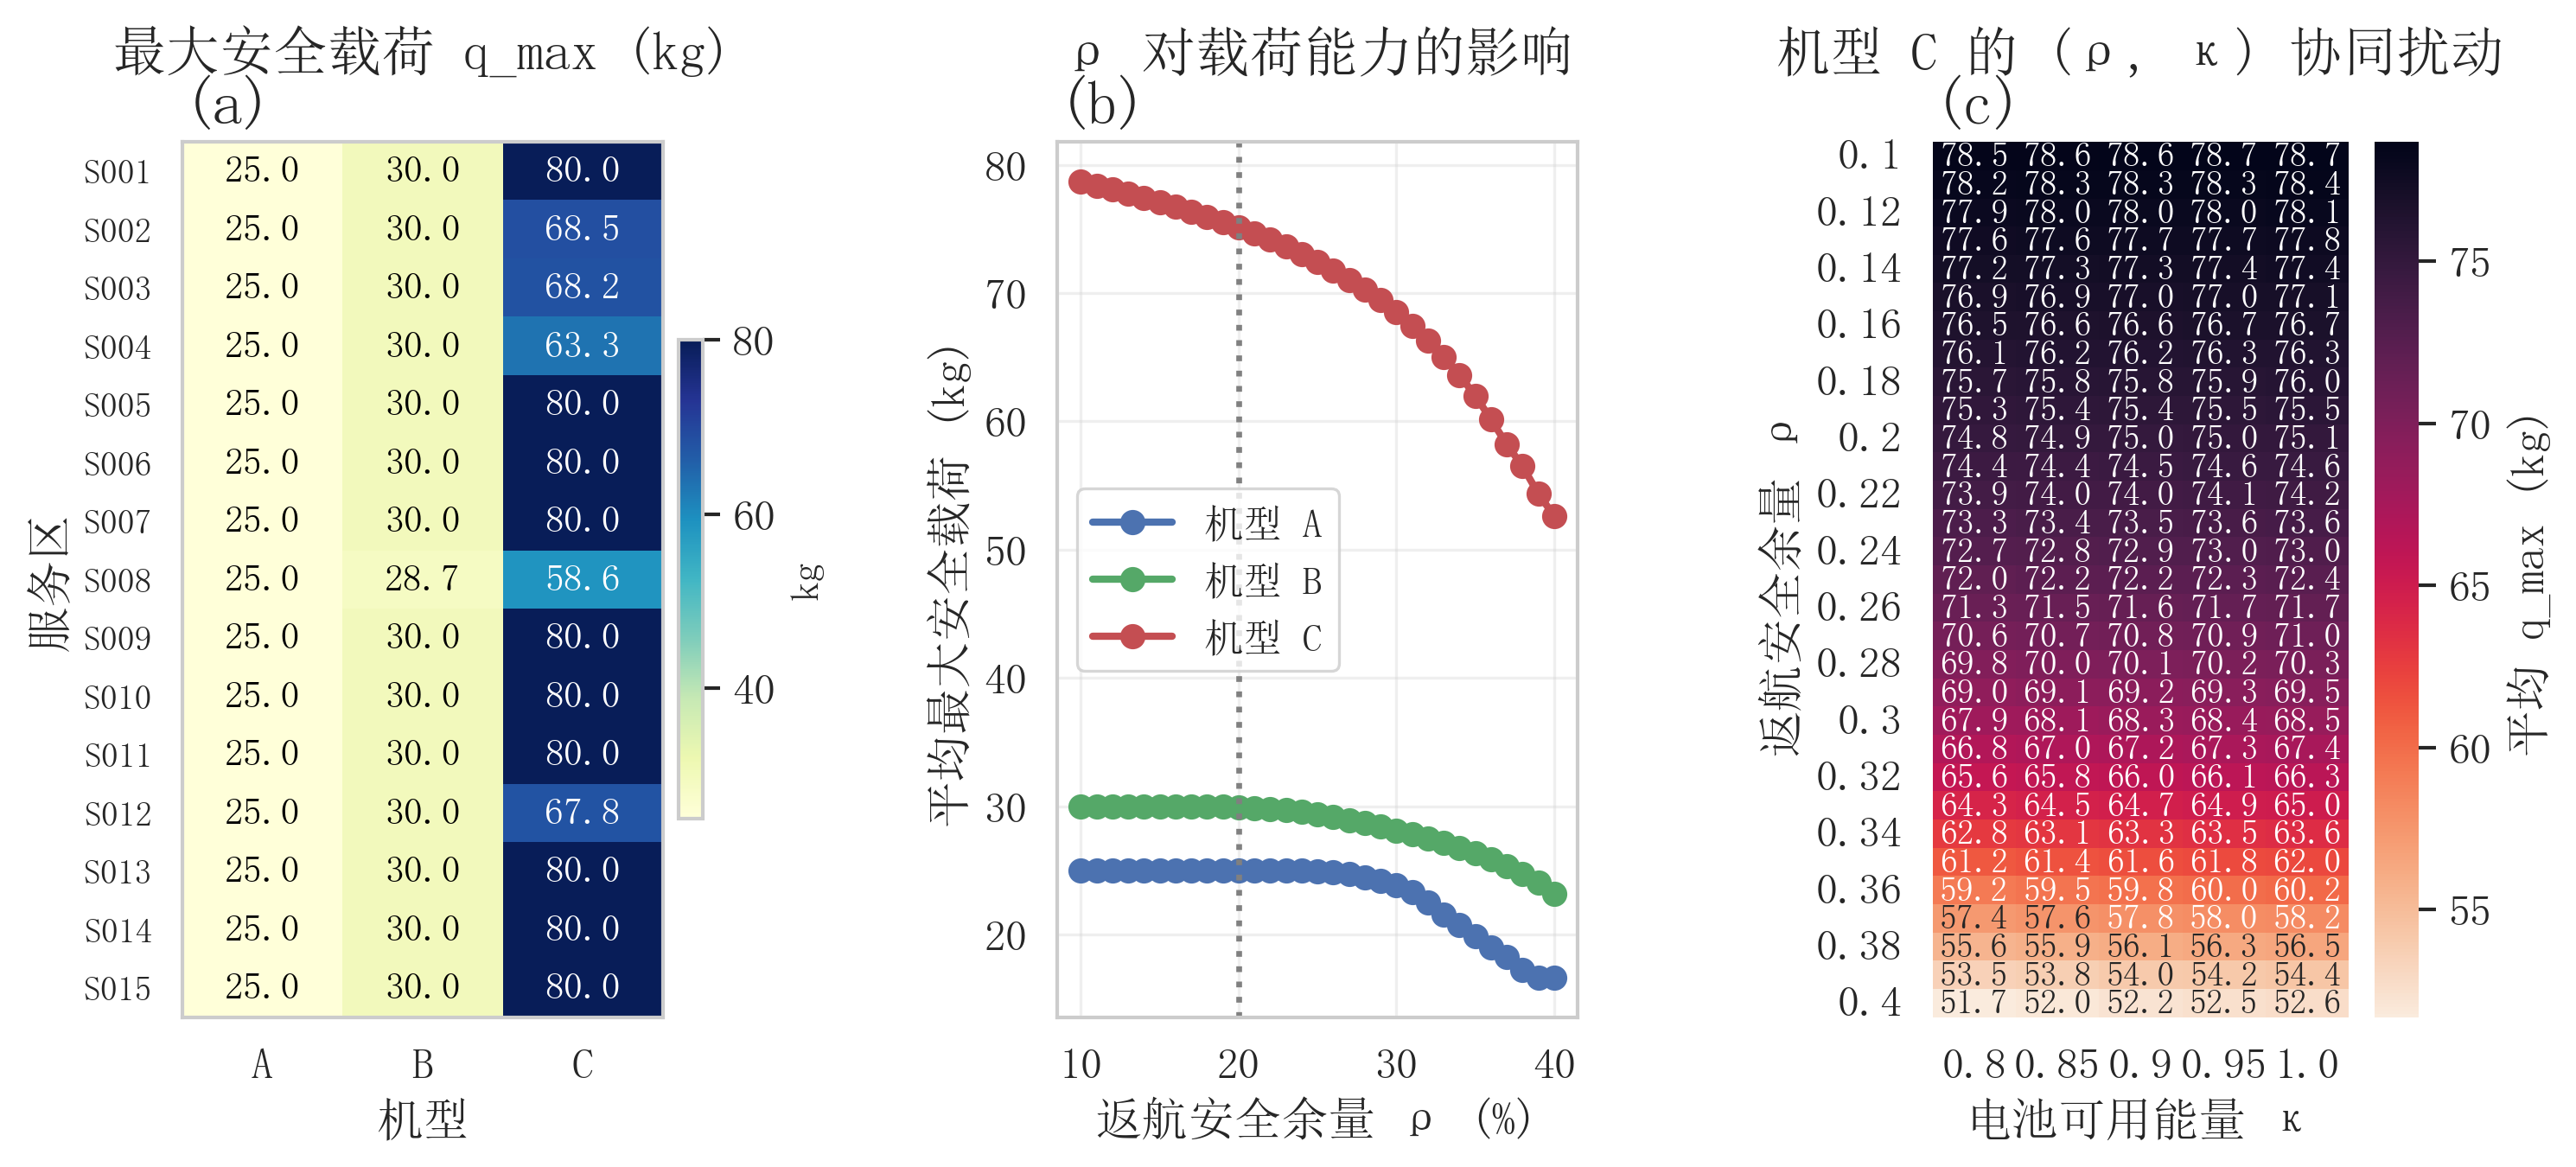
\includegraphics[width=0.95\textwidth]{figures/fig_q1_payload.png}
	\caption{最大安全载荷分布与双参数扰动}
	\label{fig:q1-payload}
\end{figure}

\subsection{货箱组批与优化}

在每个服务区内部，货箱不可拆分、不得跨服务区组批，需满足质量不超过最大安全载荷、体积不超过机型可用装载体积。同一服务区内的货箱只按（质量，体积）取值区分，取值相同的货箱在质量约束、体积约束、能耗与作业时间上完全等价，故先把货箱归并为\textbf{同质类}，再枚举“一个架次可以装哪几类各几件”的全部\textbf{架次模式}，最后在“各类货箱各取多少件”的\textbf{多重集状态}上做动态规划。状态为各类已运件数的多元组，每区货箱不超过 4 个同质类且每类件数有限，故状态空间不超过 $324$ 个，逐区求解耗时在毫秒量级，且给出的是该区在该机型下的\textbf{全局最优}组批。

为保证这一结论不依赖单一实现，本文用\textbf{两条独立路径}复核（结果见 \texttt{results/q1\_ilp\_gap.csv}）：其一为\textbf{指派式 0-1 整数规划}（变量为“箱 $i$ 放入架次 $j$”与“架次 $j$ 是否启用”，用 $y_{ij}\le u_j$、$u_j\le u_{j-1}$ 打破架次编号的置换对称），以最小化架次；其二为\textbf{集合划分整数规划}（先子集枚举出全部架次模式作为列，求恰好 $k$ 架次下的最小能耗），以最小化能耗。两条路径与动态规划在全部 $15\times3=45$ 个“服务区$\times$机型”组合上\textbf{逐行一致}；作为对照，若沿用降序首次适应（FFD）装箱，则在 45 个组合中有 2 个非最优（S007 与 S008 的 B 型，架次由 2 增至 3），对应能耗分别由 $3.427$ / $5.751$\,kWh 升至 $4.862$ / $8.165$\,kWh，全场景总能耗冗余约 $2.6\%$。

三种机型的全场景组批结果如表~\ref{tab:q1-batching}所示。

\begin{table}[htbp]
	\caption{三机型全场景组批结果对比}
	\label{tab:q1-batching}
	\centering
	\begin{tabular}{cccc}
		\toprule
		机型方案 & 往返架次数 & 总运输能耗（kWh） & 累计作业时间（h） \\
		\midrule
		全 A 型 & 52 & 112.371 & 24.82 \\
		全 B 型 & 35 & 68.470 & 15.47 \\
		全 C 型 & 18 & 74.061 & 9.40 \\
		\bottomrule
	\end{tabular}
\end{table}

由表可见三个指标存在明显的权衡：C 型以最少的架次（18）和最短的累计作业时间（9.40\,h）完成任务，但总能耗高于 B 型；B 型总能耗最低（68.470\,kWh）但架次增至 35、作业时间增至 15.47\,h；A 型在各指标上均劣于 B 型。据此本文推荐“大服务区用 C 型、小服务区用 B 型”的混合方案，以架次数为第一目标、能耗为第二目标：S001--S008 由 C 型承运（S001--S003 各村各需 2 架次，S004--S008 各 1 架次），S009--S015 由 B 型承运（各村 1 架次），共 18 架次、总能耗 63.180\,kWh、累计作业时间 9.173\,h——相对全 C 方案架次相同而能耗降低 $14.7\%$、时间缩短 $2.4\%$；相对全 B 方案架次减少 $48.6\%$、时间缩短 $40.7\%$ 而能耗还低 $7.7\%$，即在三个指标上同时不劣于两种单一机型方案。

进一步地，本文以架次上限为约束扫描出\textbf{帕累托前沿}（表~\ref{tab:q1-pareto}）。可见前沿非常平坦：架次由 18 增至 23（$+27.8\%$）仅换来总能耗由 $63.180$ 降至 $62.687$\,kWh（$-0.78\%$），代价是累计作业时间由 9.173\,h 增至 11.457\,h（$+24.9\%$）。这意味着在本题的能量参数下“多飞几趟以省电”几乎无效，架次数而非能耗才是运力规划的决定性指标，故取 18 架次方案为推荐方案。

\begin{table}[htbp]
	\caption{问题一组批方案的帕累托前沿}
	\label{tab:q1-pareto}
	\centering
	\small
	\begin{tabular}{ccccc}
		\toprule
		架次数 & 总能耗（kWh） & 累计作业时间（h） & 相对推荐方案能耗 & 相对推荐方案时间 \\
		\midrule
		\textbf{18} & \textbf{63.180} & \textbf{9.173} & --- & --- \\
		19 & 63.080 & 9.635 & $-0.16\%$ & $+5.0\%$ \\
		20 & 62.892 & 10.030 & $-0.46\%$ & $+9.3\%$ \\
		21 & 62.792 & 10.492 & $-0.61\%$ & $+14.4\%$ \\
		22 & 62.788 & 10.996 & $-0.62\%$ & $+19.9\%$ \\
		23 & 62.687 & 11.457 & $-0.78\%$ & $+24.9\%$ \\
		\bottomrule
	\end{tabular}
\end{table}

图~\ref{fig:q1-pareto}(a) 把表~\ref{tab:q1-pareto}的两支指标画在同一横轴上：总能耗随架次增加只是缓慢下行，累计作业时间却近似线性上升，两条曲线在 18 架次处张开的「剪刀口」直观说明了前沿为何平坦。(b) 给出各服务区自身的「架次–能耗」曲线族，纵轴取对数——不同服务区的单架次能耗量级相差很远，线性轴下小服务区的曲线会被压成一条线；可见同一服务区内换机型带来的能耗落差远大于同机型内增减架次的落差，这与前文「1 架 C 型可替代 2--3 架 B 型」的结构事实相符。(c) 则把 §5.3 的临界返航余量画成阶梯，架次数在 $\rho=0.2283$ 之前稳定在 18，此后逐级抬升。

\begin{figure}[htbp]
	\centering
	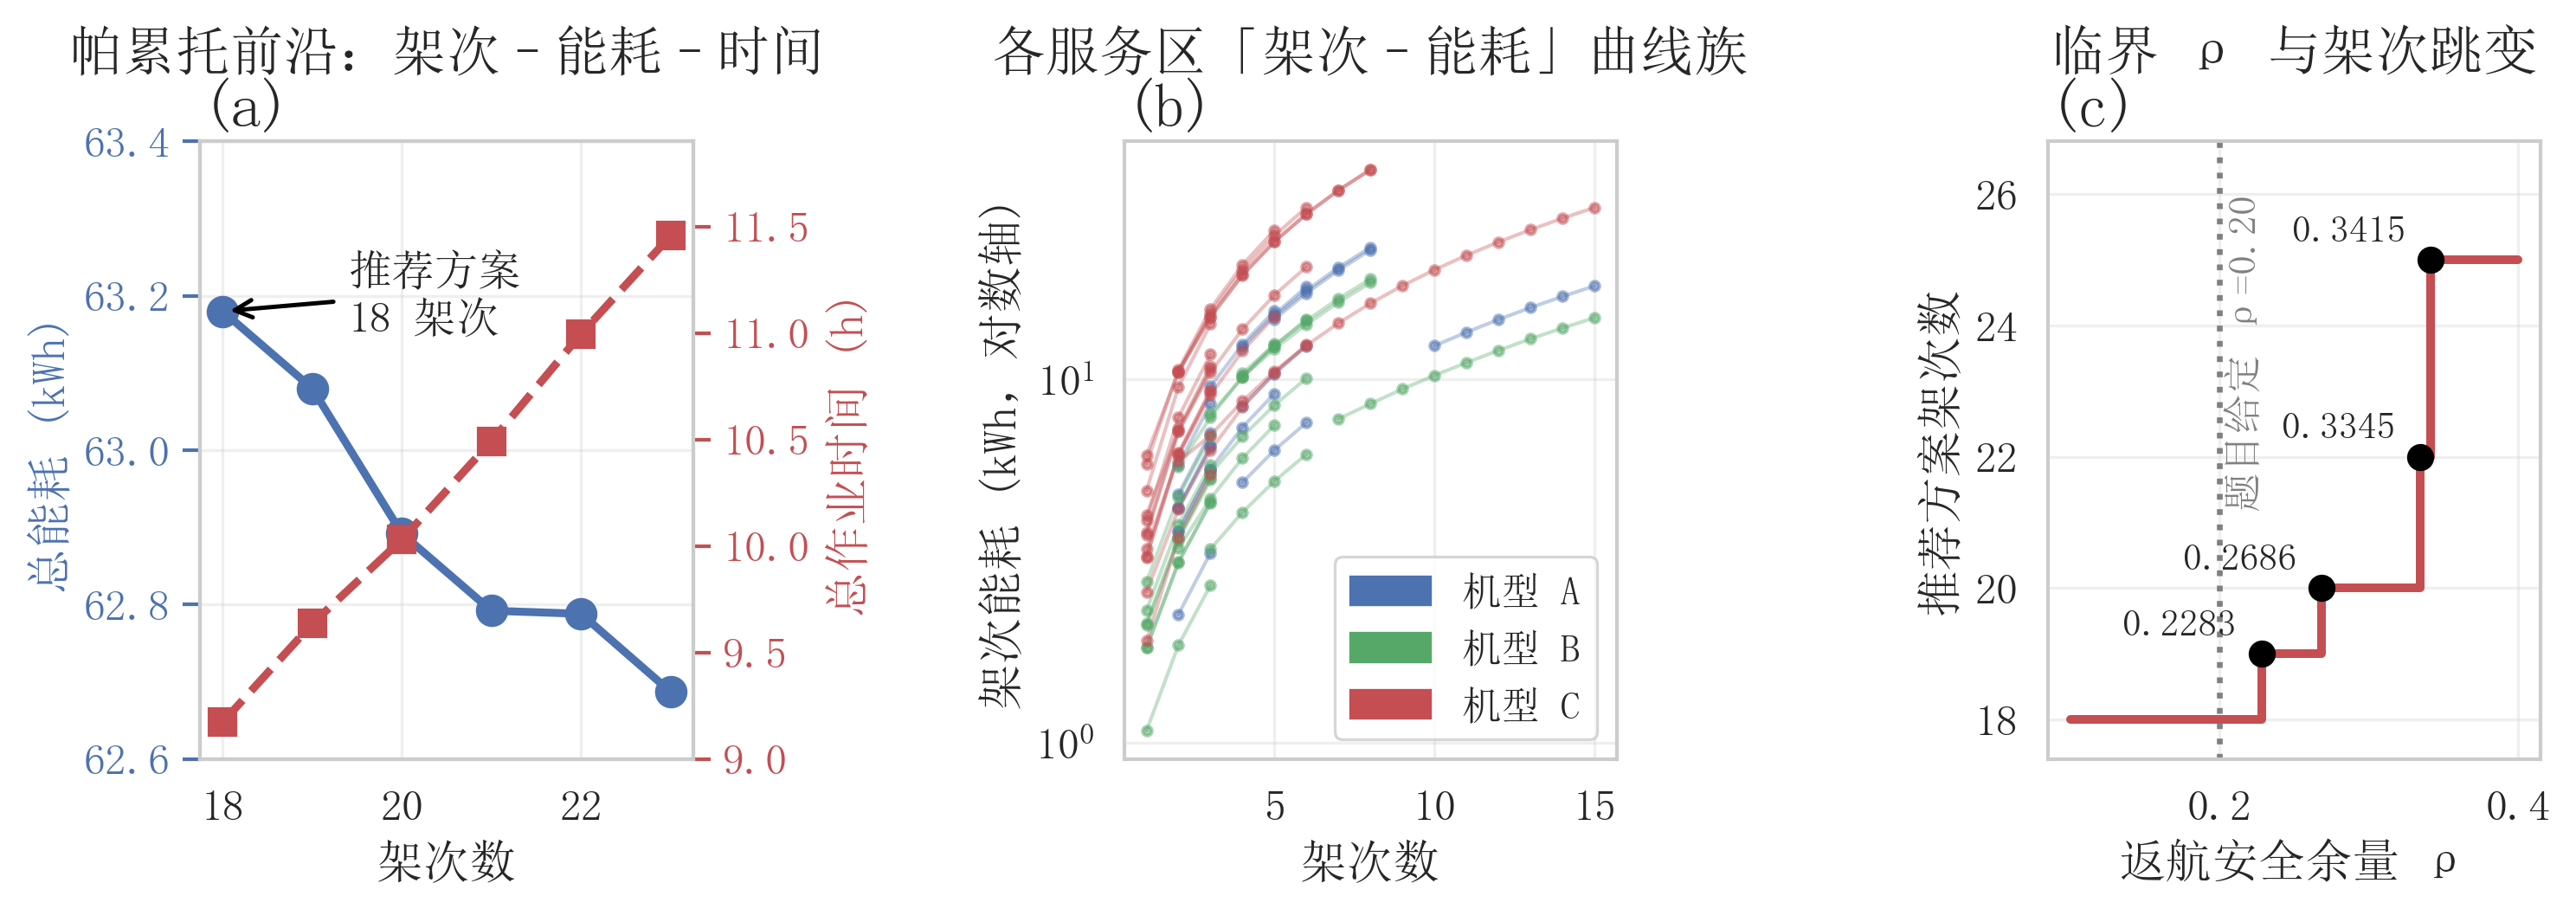
\includegraphics[width=0.95\textwidth]{figures/fig_q1_pareto.png}
	\caption{帕累托前沿、服务区曲线族与临界余量}
	\label{fig:q1-pareto}
\end{figure}

\subsection{返航安全余量的影响}

返航安全余量 $\rho_g$ 直接影响可用能量 $(1-\rho_g)E_g^{\mathrm{use}}$，进而改变最大安全载荷与组批结果。图~\ref{fig:q1-sens}给出了三种机型平均最大安全载荷随 $\rho$ 的变化。

\begin{figure}[htbp]
	\centering
	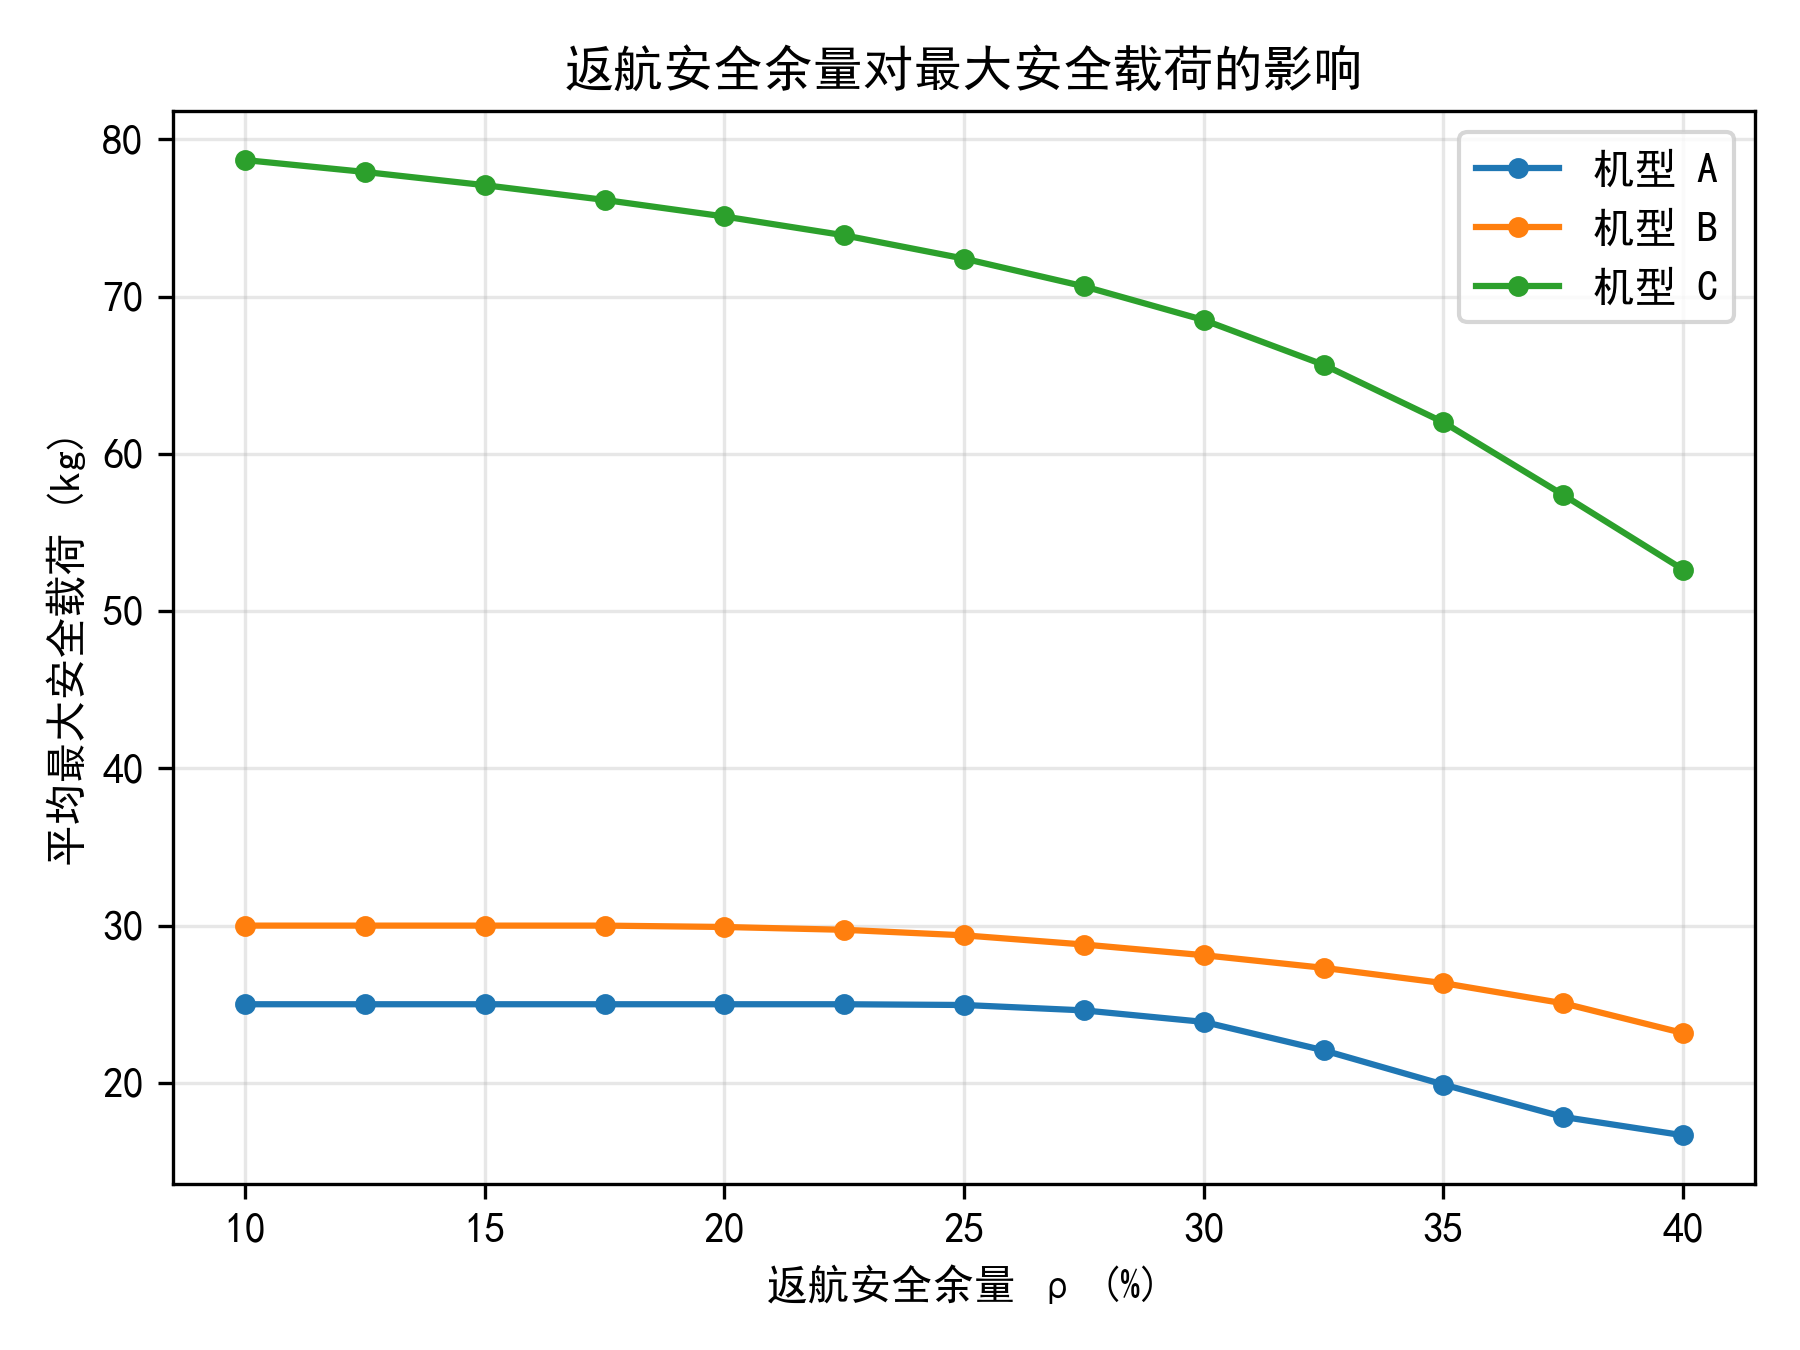
\includegraphics[width=0.62\textwidth]{figures/fig_q1_sensitivity.png}
	\caption{返航安全余量对最大安全载荷的影响}
	\label{fig:q1-sens}
\end{figure}

可见三型呈现三种不同的阶梯形态（同一条曲线亦见于图~\ref{fig:q1-payload}(b)）。A 型与 B 型在 $\rho$ 较小时是\textbf{平台}——$\rho\le0.20$ 时 A 型恒为 25.00\,kg、$\rho\le0.15$ 时 B 型恒为 30.00\,kg，说明此区间内二者的瓶颈是载质量上限而非能量，提高返航余量不损失运力。C 型则自始受能量约束，平均最大安全载荷由 $\rho=0.10$ 时的 78.68\,kg 单调降至 $\rho=0.40$ 时的 52.64\,kg（$\rho$ 每增大 10\% 平均下降约 8.7\,kg，与表~\ref{tab:sens}一致），且下降在 $\rho>0.30$ 后明显加速。

以总架次数为观测量对 $\rho$ 做二分定位，可得组批方案的\textbf{临界点}：$\rho=0.2283$ 时总架次由 18 跳至 19，此后 $0.2686$、$0.3345$、$0.3415$ 依次跳至 20、22、25 架次；当 $\rho$ 超过 $0.3513$ 时方案整体失效——此时最不利服务区 S008 对三种机型均已不可达。分机型看，S008 的作业可行性上界为 A 型 $0.2992$、C 型 $0.3510$、B 型 $0.3513$，即\textbf{率先失效的是航程最短、能量最小的 A 型}（$\rho>0.2992$ 后 A 型空载亦无法往返 S008），随后才是 C 型与 B 型。这意味着提高安全余量对运力的压缩不是均匀的：它先剥夺小型机的可达性、再压缩重载机的有效载荷，二者叠加使架次数阶梯式上升，安全性与运输效率需要在上述临界点之间权衡。
         % 五、问题一
\section{问题二：异构无人机多点多架次调度}

\subsection{模型建立}

在问题一基础上，问题二允许每个架次访问多个服务区并返回 O01，联合确定货箱组批、服务区访问顺序、机型、执行无人机、共享电池与各架次开始时刻。决策变量为：货箱 $c$ 是否由架次 $p$ 运输（$y_{cp}\in\{0,1\}$）、架次 $p$ 的服务区访问顺序 $\sigma_p$、架次 $p$ 的机型选择 $z_{pg}\in\{0,1\}$、开始时刻 $t_p$，以及架次 $p$ 所占用的无人机与共享电池。记 $\mathcal{P}$ 为架次集合、$\mathcal{C}$ 为货箱集合、$\mathcal{B}_g$ 为机型 $g$ 的共享电池池、$g(p)$ 为架次 $p$ 所选机型、$T^{\mathrm{deliver}}_c$ 为货箱 $c$ 的实际交付时刻、$D_c$ 与 $B_c$ 为其医疗期望时刻与首批截止时刻，则可行域由下列七条界定。

\begin{itemize}
	\item[(C1)] \textbf{货箱唯一投送且不可拆：}$\sum_{p\in\mathcal{P}} y_{cp}=1,\ \forall c\in\mathcal{C}$。货箱在架次内不再分包，也不允许同一箱分投两处。
	\item[(C2)] \textbf{载质量与装载体积：}$\sum_{c}m_c\,y_{cp}\le Q_{g(p)}$ 且 $\sum_{c}v_c\,y_{cp}\le V^{\mathrm{load}}_{g(p)}$，$\forall p$。右端是\textbf{架次所选机型}的容量，而机型本身是决策变量，故该约束的右端随 $z_{pg}$ 切换；三个机型的可用装载体积为 $0.06$ / $0.073$ / $0.25$\,m$^3$。
	\item[(C3)] \textbf{返航能量余量：}$E^{T}_p\le\bigl(1-\rho_{g(p)}\bigr)E^{\mathrm{use}}_{g(p)}$，$\forall p$（式~\eqref{eq:energy-margin}）。多区架次的载荷随沿途投送递减，故 $E^{T}_p$ 由逐航段能耗累加得到，而不是按满载全程估算。
	\item[(C4)] \textbf{机型对应的无人机与电池库存：}任一时刻在役的架次数不超过该机型的可用无人机数（全队 8 架，A/B/C 三型各 $4/2/2$ 架），共享电池按机型分池、在役组数不超过池内库存（A/B/C 各 $6/4/4$ 组）。这一条把「机型」与「机队资源」绑在一起，是问题二区别于经典多车场 VRP 的关键：选型不能只看单架次能耗，还要看该型机队是否被别的架次占住。
	\item[(C5)] \textbf{电池充电周转：}每次充电的占用时长按式~\eqref{eq:charging} 的两阶段模型计算，同一组电池的放电占用与充电时段不得重叠；充电占用一并进入资源链传播，即某架次的可用起飞时刻取决于其电池在上一次占用结束后的充电完成时刻。
	\item[(C6)] \textbf{硬时限：}$T^{\mathrm{deliver}}_c\le D_c$（医疗物资）且 $T^{\mathrm{deliver}}_c\le B_c$（首批保障物资），$\forall c\in\mathcal{C}_{\mathrm{med}}\cup\mathcal{C}_{\mathrm{bat}}$。其余货箱的期望送达时刻不进约束，只以加权时延衡量配送及时性。
	\item[(C7)] \textbf{货箱不得跨服务区组批：}$\forall c\in\mathcal{C},\ \forall p:\ y_{cp}=1 \Rightarrow c$ 所在的服务区属于架次 $p$ 的服务区集合，即货箱只与其同一服务区内的货箱并入同一架次，不得跨区拼箱。这一条与问题一的题面约束是同一条，此处并非新增收紧，而是\textbf{求解器已在执行、此前未写进模型}的一条：组批由以服务区为键的数据结构强制（\texttt{code/q2.py} 的 \texttt{merge\_nonurgent} 按服务区归并货箱），货箱在数据结构上无法被换到别的服务区。把它显式列出，问题一与问题二的组批可行域才是同一个。
\end{itemize}

与前期的构造式方案不同，本文把 (C6) 的两类时限处理为\textbf{硬约束}而不是罚项：任一货箱超出其医疗期望时刻或首批截止时刻，该解即判为不可行（目标值取 $+\infty$）并从解空间中剔除，报告前再以断言强制校验硬违约数为 0；只有第三类时限作为软目标进入加权时延 $F_{\mathrm{delay}}=\sum_c w_c L_c$，其中 $L_c=\max(0,\,T_c^{\mathrm{deliver}}-T_c^{\mathrm{expect}})$。这样处理之后，“零违约”就不再是某次运行的幸运结果，而是解空间的定义本身。

优化目标为 $F=w_1 F_{\mathrm{delay}}/R_{\mathrm{delay}}+w_2\,T_{\mathrm{make}}/R_{\mathrm{make}}$，即\textbf{时效优先}：先保证硬时限零违反，再权衡加权时延与全部任务完成时间；架次数与能耗不进入目标，而是作为代价如实报告（处理方式见 6.2 节的 $\varepsilon$-约束）。式中权重取 $w_1=1.0$、$w_2=0.30$，两项各按\textbf{构造基线解自身的取值}归一化，即 $R_{\mathrm{delay}}=\max\{F_{\mathrm{delay}}^{\text{基线}},\,1\}$、$R_{\mathrm{make}}=\max\{T_{\mathrm{make}}^{\text{基线}},\,1\}$。这样取是因为时延以秒计、完工时间亦以秒计，二者量级相近却\textbf{不同源}：用各自的基线值作标度，权重才表达“单位相对改进”的交换比，而不是被量纲差掩盖。以构造基线为标度的另一个好处是权重不必随算例规模重新标定——基线本身就是同一算例的参考水平。$w_2/w_1=0.30$ 表示\textbf{一比一权衡下}，宁可多等 1 单位相对时延以换取 0.3 单位相对完工时间。这里必须讲清楚一件事：按基线值归一化后，两项的边际交换比被固定为 $0.30\,R_{\mathrm{delay}}/R_{\mathrm{make}}$，在本算例的基线上折算下来是“1\,s 完工抵十余秒时延”——\textbf{这与题面「及时性优先、其次完工、最后能耗与架次」的次序并不一致}。故本文对 $F$ 的定位是\textbf{搜索的下坡方向}，而不是最终取舍：$F$ 提供的平滑梯度用于让 ALNS 稳定收敛，\textbf{最终择档改用题目优先级的字典序}（式~\eqref{eq:q2-key}），两把尺子的分工见 6.2 节第 (6) 条。此外，$\varepsilon$-约束扫描时对超出架次数上界 $\varepsilon$ 的部分施加线性罚 $0.50\,(\text{架次}-\varepsilon)$，用于把搜索压回该档的可行域，档内最终解仍须满足架次数 $\le\varepsilon$ 并复检（见 6.2 节）。

\subsection{求解策略}

鉴于问题规模与约束耦合，本文采用“构造基线 + 大邻域自适应搜索（ALNS）+ $\varepsilon$-约束扫描”的求解框架，并另做两层小规模精确验证。

\textbf{（1）求解框架与精确组批初始解。}本文的求解链为“精确组批 $\to$ 路线全排列精化 $\to$ 瓶颈感知解码 $\to$ ALNS 破坏—修复搜索 $\to$ $\varepsilon$-约束逐档扫描 $\to$ 逐档定型 $\to$ 按题目优先级择档”，如图~\ref{fig:q2-algorithm}所示。初始架次集合不再由贪心规则给出，而是对每个服务区做一次\textbf{精确装箱}：先枚举该区非紧急货箱的全部“载质量—体积”可行子集，再用子集 DP（状态压缩）求字典序（批次数 $\to$ 能耗和 $\to$ 时间和）最优的划分；候选池由 A/B/C 三型各自的可行子集按货箱掩码合并去重、逐掩码保留机队代价最优的机型构成，于是重载子集自然由 C 型承载，轻载子集则可能由 A/B 型以更低能耗承载。紧急货箱（医疗与首批）仍按“每区单独成架次”构造——这条是硬时限的保证，不交给搜索去试探。区箱数超过 16 或存在单箱超限时回退 FFD，以免子集枚举规模失控。该初始解只作为搜索起点，其质量由 6.4 节的精确解标定。

这里须交代一处实现口径，它关系到「表里的解」与「落盘的解」是不是同一个：\textbf{搜索内核}（破坏—修复主循环、可行档案与接受准则）沿用本文 \texttt{code/q2.py} 的 \texttt{alns}，v2 引擎替换的是它的三层外围——\textbf{构造层}（精确组批取代 FFD 构造）、\textbf{解码层}（\texttt{q2.schedule(dispatch="balanced")}，把选型记账统一到一处）、\textbf{派工择序层}（插入式局部寻优与退火搜索），并加上多种子与档间热启动；逐档解在落盘前还要过 7.4 节的中继门禁重排。只换外围而不换内核，是因为内核的接受准则与可行档案决定了「搜索途中路过的可行好解不会被丢掉」这一性质；外部实现把这两条改成「不可行解一律不接受、只留末端最优」，本文\textbf{没有}移植，否则会凭空损失可行解。

% 画布 816×384 px，横版三栏（宽高比 2.13），与图 2.1《总技术路线图》同宽同字号；
% 按 \textwidth 插入后图内文字约 9.5 pt。源文件由 code/make_q2_algorithm.py 生成。
\begin{figure}[htbp]
	\centering
	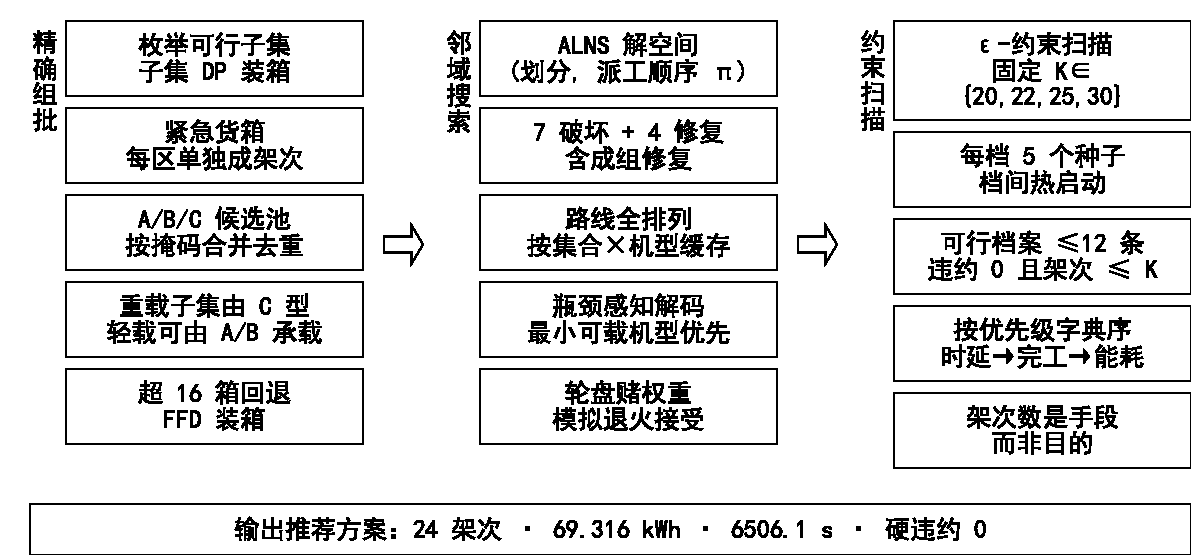
\includegraphics[width=\textwidth]{figures/fig_q2_algorithm.pdf}
	\caption{问题二求解框架}
	\label{fig:q2-algorithm}
\end{figure}

\textbf{（2）路线全排列与瓶颈感知解码。}给定一架次所服务的服务区集合，其访问顺序仍有 $k!$ 种可能；服务区数不超过 5 时（$5!=120$）本文对全部排列精确枚举，硬时限箱以最早交付为平局键，结果按“服务区集合 $\times$ 机型”缓存复用。解码（把架次集合落成“哪架无人机、哪组电池、几点起飞”）同样不是逐架次贪心：调度函数 ${\rm schedule}(d,\mathcal{T},\pi)$ 接受一个派工优先级排列 $\pi$ 并做\textbf{瓶颈感知选型}——在 $\pi$ 给定的次序下，候选机型的评分为「开始时刻 $+300\times$ 机型重载序」（A/B/C 记 $0/1/2$），即在 $300$\,s 的让位窗口内优先把架次派给\textbf{装得下的最小}机型，同分再比能耗。这一项之所以必要，是因为“能耗最小”的机型未必是机队瓶颈所在：C 型每箱公里最省电，若一味按能耗选型，总时长会堆到只占机队四分之一的 2 架 C 型机上，完工时刻被该机型的串行时长钉死，而与总工作量无关。仅改变 $\pi$ 就会改变无人机与电池的可用时刻，进而同时改变架次数、能耗与完成时间三个指标——实测把 $\pi$ 由“紧迫度升序”换成“最早完成时刻优先”即可使完成时间下降约 $2\%$。故本文的解空间定义为 $(\text{货箱}\to\text{架次的划分},\ \pi)$ 二元组。

\textbf{（3）ALNS 的破坏与修复算子。}在上述解空间上实施自适应大邻域搜索\cite{pisinger2007general}，共 \textbf{7 个破坏算子}：随机移箱、Shaw 相关移箱（按时空邻近性成簇摘除）、最差架次整体拆除、按服务区整体移除、仅移除非紧急货箱、整架次拆解、以及仅扰动顺序而不动划分；配 \textbf{4 个修复算子}：贪婪插入、Regret-2 插入、新开架次、以及成组修复。算子权重按轮盘赌自适应更新（段长 100 次迭代、平滑系数 $\rho=0.25$），接受准则采用归一化目标上的几何降温模拟退火。其中“成组修复”是为解决下述代理代价缺陷而专门加入的：贪婪插入用“该架次最省机型代价”作为插入位置的代理代价，而该代理假设每架次可自由选用最省机型，\textbf{看不到机队资源竞争}，会系统性地漏掉“并区以腾出紧缺机型”这类协同动作。成组修复改为对候选前 $10$ 个位置做真实解码评估，代价更高但能看见资源竞争。

上述破坏—修复算子、$\varepsilon$-约束逐档扫描与消融对照的实测表现汇总于图~\ref{fig:q2-alns}，该图并排给出收敛轨迹、消融比值与四档非支配关系三张诊断。

% 图片宽度 10.0 in，按 0.95\textwidth=6.17 in 插入，缩放比 0.617
\begin{figure}[htbp]
	\centering
	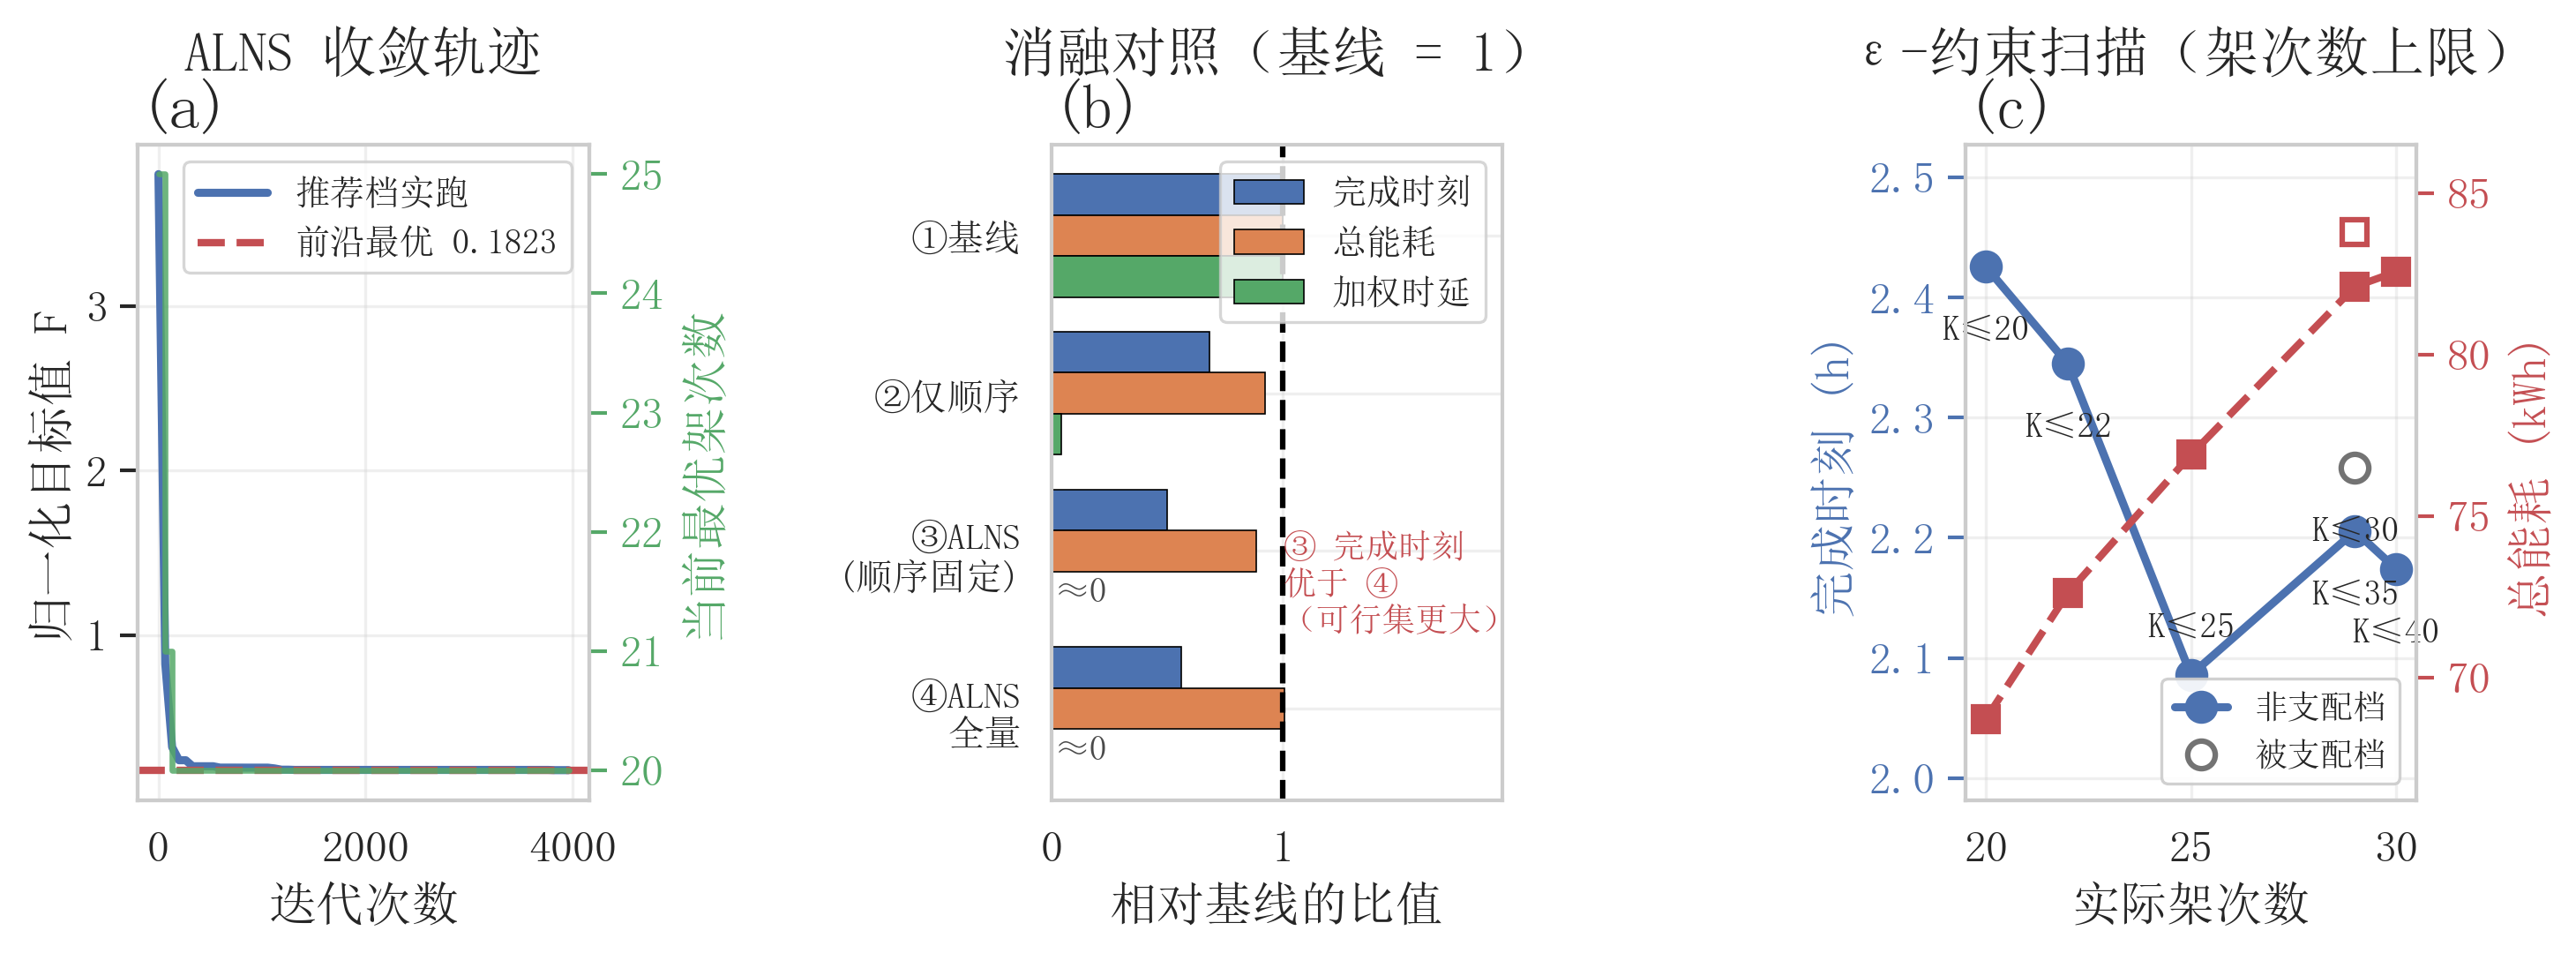
\includegraphics[width=0.95\textwidth]{figures/fig_q2_alns.png}
	\caption{ALNS 收敛、消融对照与 $\varepsilon$-约束扫描}
	\label{fig:q2-alns}
\end{figure}

图~\ref{fig:q2-alns}给出搜索过程的三项诊断：(a) 推荐档（$K\le25$）\textbf{那一次真实运行}的目标值收敛曲线（每 $58$ 次迭代记一点的抽样记录），其终值 $0.145602$ 与表~\ref{tab:q2-pareto}中 $K\le25$ 档的目标值一致，即曲线确为所求方案本身的轨迹；实测全部 $4$ 次改进都发生在第 $465$ 次迭代之前，此后连续 $1\,500$ 轮档案无改进、触发耐心早停，该档于第 $1\,973$ 次迭代终止（故轨迹短于 $3\,500$ 轮的预算上限，这是早停而非记录缺失）——可见预算的绝大部分用于确认而非改进；(b) 表~\ref{tab:q2-ablation}五项消融的并排对照，三项指标一律化成\textbf{相对基线①的比值}才画得进同一张图（量纲相差几个数量级）——除④的总能耗高于基线（比值 $1.054$）外，其余各项都落在 $1.0$ 左侧，③的加权时延被压到 $0$ 故在柱位上就地标出「$\approx 0$」，读者一眼可看出“顺序”与“组批”各自解决了什么；(c) 四个档位的架次数—能耗—完成时间扫描，其中\textbf{实心点}连线的是四维非支配档，\textbf{空心点}为被支配档——被支配关系连同各档指标一并列于表~\ref{tab:q2-pareto}，读者可逐档核对。

\textbf{（4）$\varepsilon$-约束逐档扫描。}架次数是手段而非目的，且与时延、完成时间直接对抗，故不把它与时延平权加权，而是取为约束逐档扫描：固定架次数上限 $K\in\{20,22,25,30\}$，在各档内最优化时效目标。这里 $K$ 是\textbf{货真价实的约束}：搜索中间态允许暂时超出 $K$，以便破坏算子拆散架次后重新合并，但每一档的候选解只从“硬违约数为 $0$ 且实际架次数 $\le K$”的\textbf{可行档案}中录取，导出前再复检一次；某档若全程未找到可行解，则如实记为该档无解，不以超 $K$ 的方案顶替。每档独立运行 5 个随机种子（种子取 $20260923+101K+7919s$，互不重叠），并把上一档的最优解热启动进下一档；档案按（架次、完成时间、能耗、时延）去重，上限 12 条。

档位上限为什么收到 30 而不更大：\textbf{通信连续性是问题三的硬约束}，而需要同时护航的运输架次会随架次数上升。这一收窄来自上一轮更宽扫描（六档，原始记录见 \texttt{\_legacy/q2\_v1/q2\_pareto.csv}）的实测：$K\le35$ 与 $K\le40$ 两档的完成时间更短，但其并发中继需求峰值达 3，已超过题给的 2 架中继无人机，问题三只能以中断收场。故本文把档位收窄到 $K\in\{20,22,25,30\}$——即扫描过的六档中“问题三可零中断”的那四档——再在其中择档，否则会出现“问题二指标更优、整卷方案却违反硬约束”的自相矛盾。需要说清的是：本轮只重跑了收窄后的四档，宽档的两条记录是上一轮同口径扫描的结果，作为问题二—问题三耦合的实测证据在 7.6 节引用，本文不把它表述为“已证明 $K\le35$ 必然中断”。

\textbf{（5）逐档定型轮。}档案里的解是搜索途中的快照，其派工顺序未必已经收敛。故对\textbf{每一档}的代表解再跑一轮定型：先做派工顺序的插入式局部寻优（架次集合不变，接受准则为完成时间、能耗、加权时延三项的严格 Pareto 改进，故不可能变差），再做一轮退火派发顺序搜索，用于消掉“必须让中间态先变差才腾得出来的尾部”。两轮都只动 $\pi$，路线与架次数不变，$K$ 档约束仍成立。之所以逐档都做、而不是只做最终被选中的那一档，是因为交付的推荐方案就是其中一档：若各档定型程度不一，档间比较就失去可比性，而且“表里那一行”与“落盘的方案”就不再是同一个解。

\textbf{（6）择档键按题目优先级字典序。}搜索使用的标量目标 $F$ 把加权时延与完成时间按 $w_1\!:\!w_2$ 折算，用于给搜索提供平滑的下降方向；但\textbf{折算本身会引入交换比}——两项参考量相差一个量级，等价的边际权重并不符合题目给定的“及时性优先、其次完工、最后能耗与架次”次序。故\textbf{终选不沿用 $F$}，而是按题目优先级逐层比较
\begin{equation}
	\text{key}=\bigl(\ \text{加权时延},\ \text{完成时间},\ \text{总能耗},\ \text{架次数},\ K\ \bigr),
	\label{eq:q2-key}
\end{equation}
前一层严格更优即定胜负；同层内相差小于 $10^{-6}$ 视为并列（不让浮点噪声决定胜负），继续比下一层。两把尺子分工明确：$F$ 管搜索方向，式~\eqref{eq:q2-key} 管最终取舍；逐档定型的代表解在式~\eqref{eq:q2-key} 下最优者即为推荐方案。本问的求解规模为：80 个货箱、8 架无人机、14 组共享电池，解空间是「80 箱到架次的划分 $\times$ 派工排列 $\pi$」的二元组；单次搜索 3\,500 轮迭代、7 个破坏算子与 4 个修复算子，$\varepsilon$-约束取 $K\in\{20,22,25,30\}$ 四档、每档 5 个种子，合计 20 次独立搜索；精确验证两层中，分区层为集合划分整数规划、时序层为 big-$M$ 析取 MILP，算例规模见 6.4 节。

\subsection{求解结果}

按式~\eqref{eq:q2-key}的题目优先级字典序，本文取 $K\le25$ 一档作为推荐方案：共 \textbf{24 个运输架次}，全部 80 个货箱在硬时限内完成交付（医疗期望与首批保障违约数均为 $0$，加权时延为 $0$），总运输能耗 $69.316$\,kWh，全部任务完成时间 $6506.1$\,s（$1.81$\,h）。资源使用情况为：8 架实体无人机全部投入使用，14 组共享电池参与周转（A/B/C 型分别为 6/4/4 组），与库存完全一致，满足资源可行性。24 个架次中有 3 个访问两个服务区（T08: S010$\to$S014、T12: S001$\to$S010、T21: S011$\to$S008），正是这几条跨区架次把 15 个服务区绑定为问题四所需的原子任务单元（见 8.1 节）。调度甘特图如图~\ref{fig:q2-gantt}所示。

\begin{figure}[htbp]
	\centering
	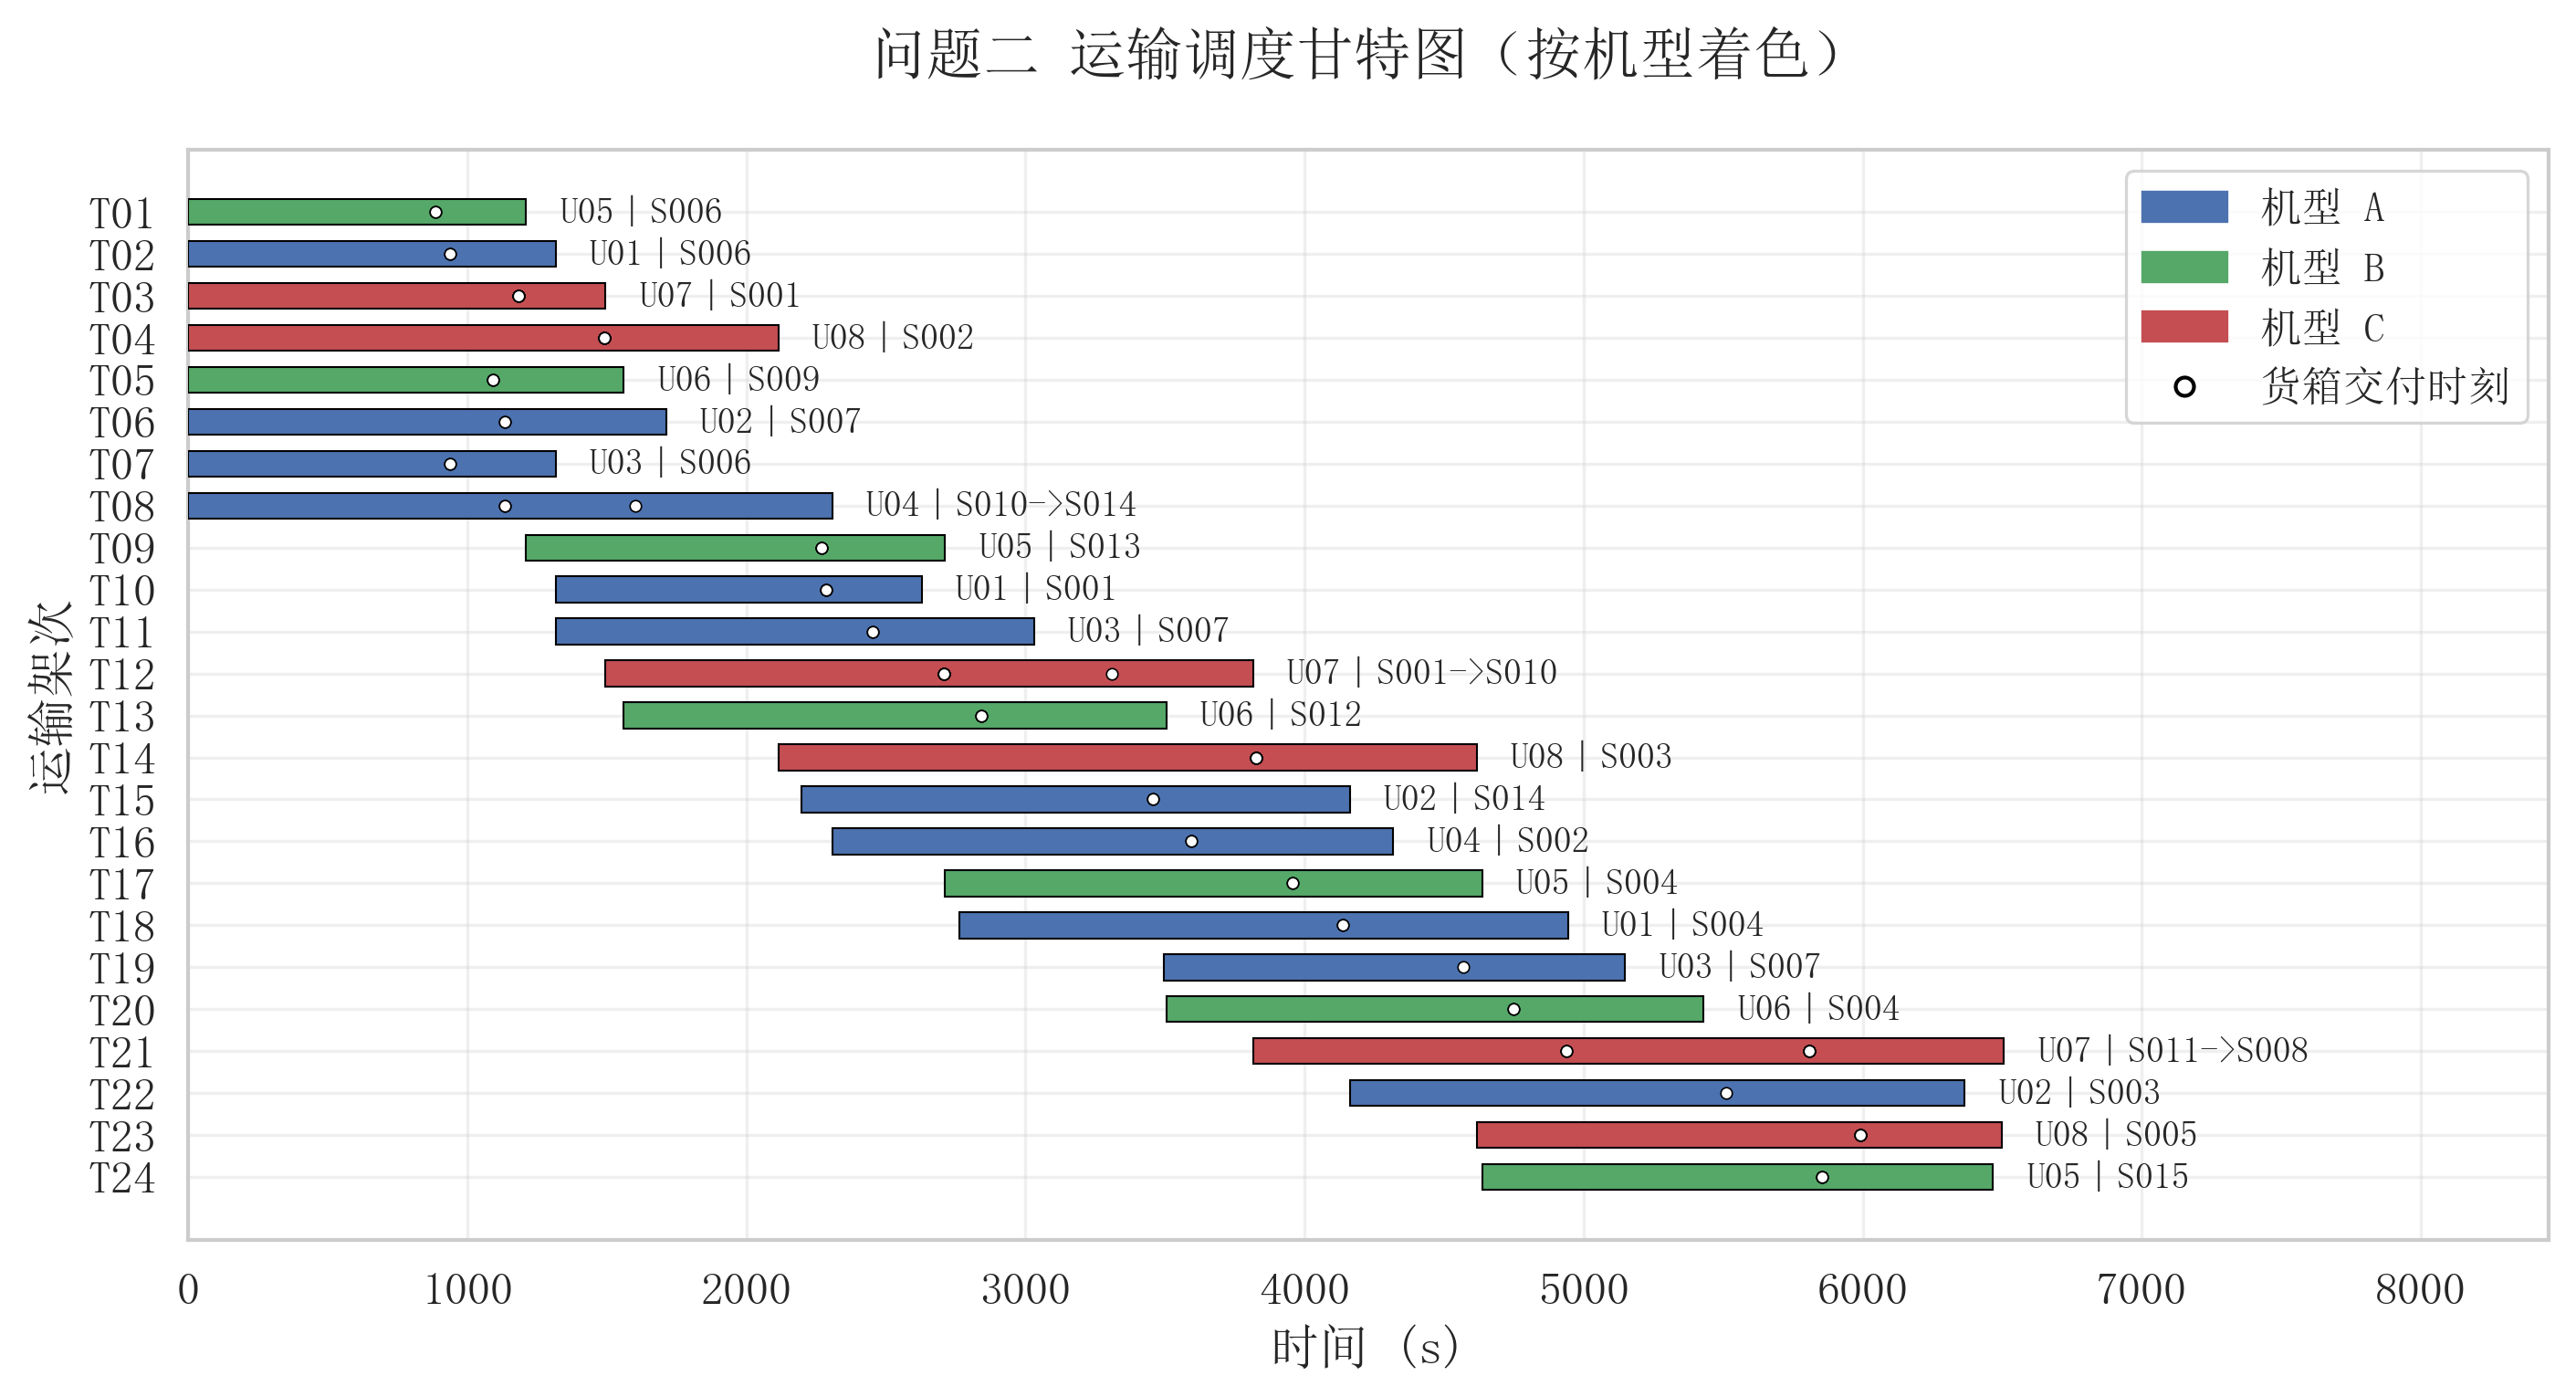
\includegraphics[width=0.92\textwidth]{figures/fig_q2_gantt.png}
	\caption{问题二推荐方案运输调度甘特图}
	\label{fig:q2-gantt}
\end{figure}

图~\ref{fig:q2-gantt}把 24 个架次按机型铺在一条共享时间轴上，横轴刻度即任务时钟，条右端的空心圆圈是该架次货箱的交付时刻。从图中可读出四点。其一，\textbf{交付时刻一律落在条的内部而非右端}——圆圈之后仍有长度，那就是投送完成后的返航段，这条「先送后回」的顺序在全部 24 条上一致，说明时限是按交付（而非返航）核对的。其二，\textbf{T08、T12、T21 三条明显长于同机型其余架次}，它们正是访问两个服务区的跨区架次，也是把 15 个服务区绑定为问题四原子任务单元的那三条（8.1 节）。其三，\textbf{时间轴上没有出现超过单个架次时长的空档}：第一个架次在起点附近起飞、最后一个架次的结束时刻与 $6506.1$\,s 的完工时刻一致，说明 8 架无人机与 14 组电池确实被连续周转使用，机队利用率的提升来自排程而非闲置。其四，\textbf{同一架无人机的多个架次在时间上首尾相接而不重叠}——例如 U08 依次承担 T04、T14、T24，U07 依次承担 T03、T12、T21——这正是 §6.1 约束 (C4)(C5) 中「无人机与电池占用区间不得重叠」在解上的体现；若把机型指派改动一处，这几条平行束的归属会立刻改变，故它同时是机队约束被真正执行的图示证据。

\begin{figure}[htbp]
	\centering
	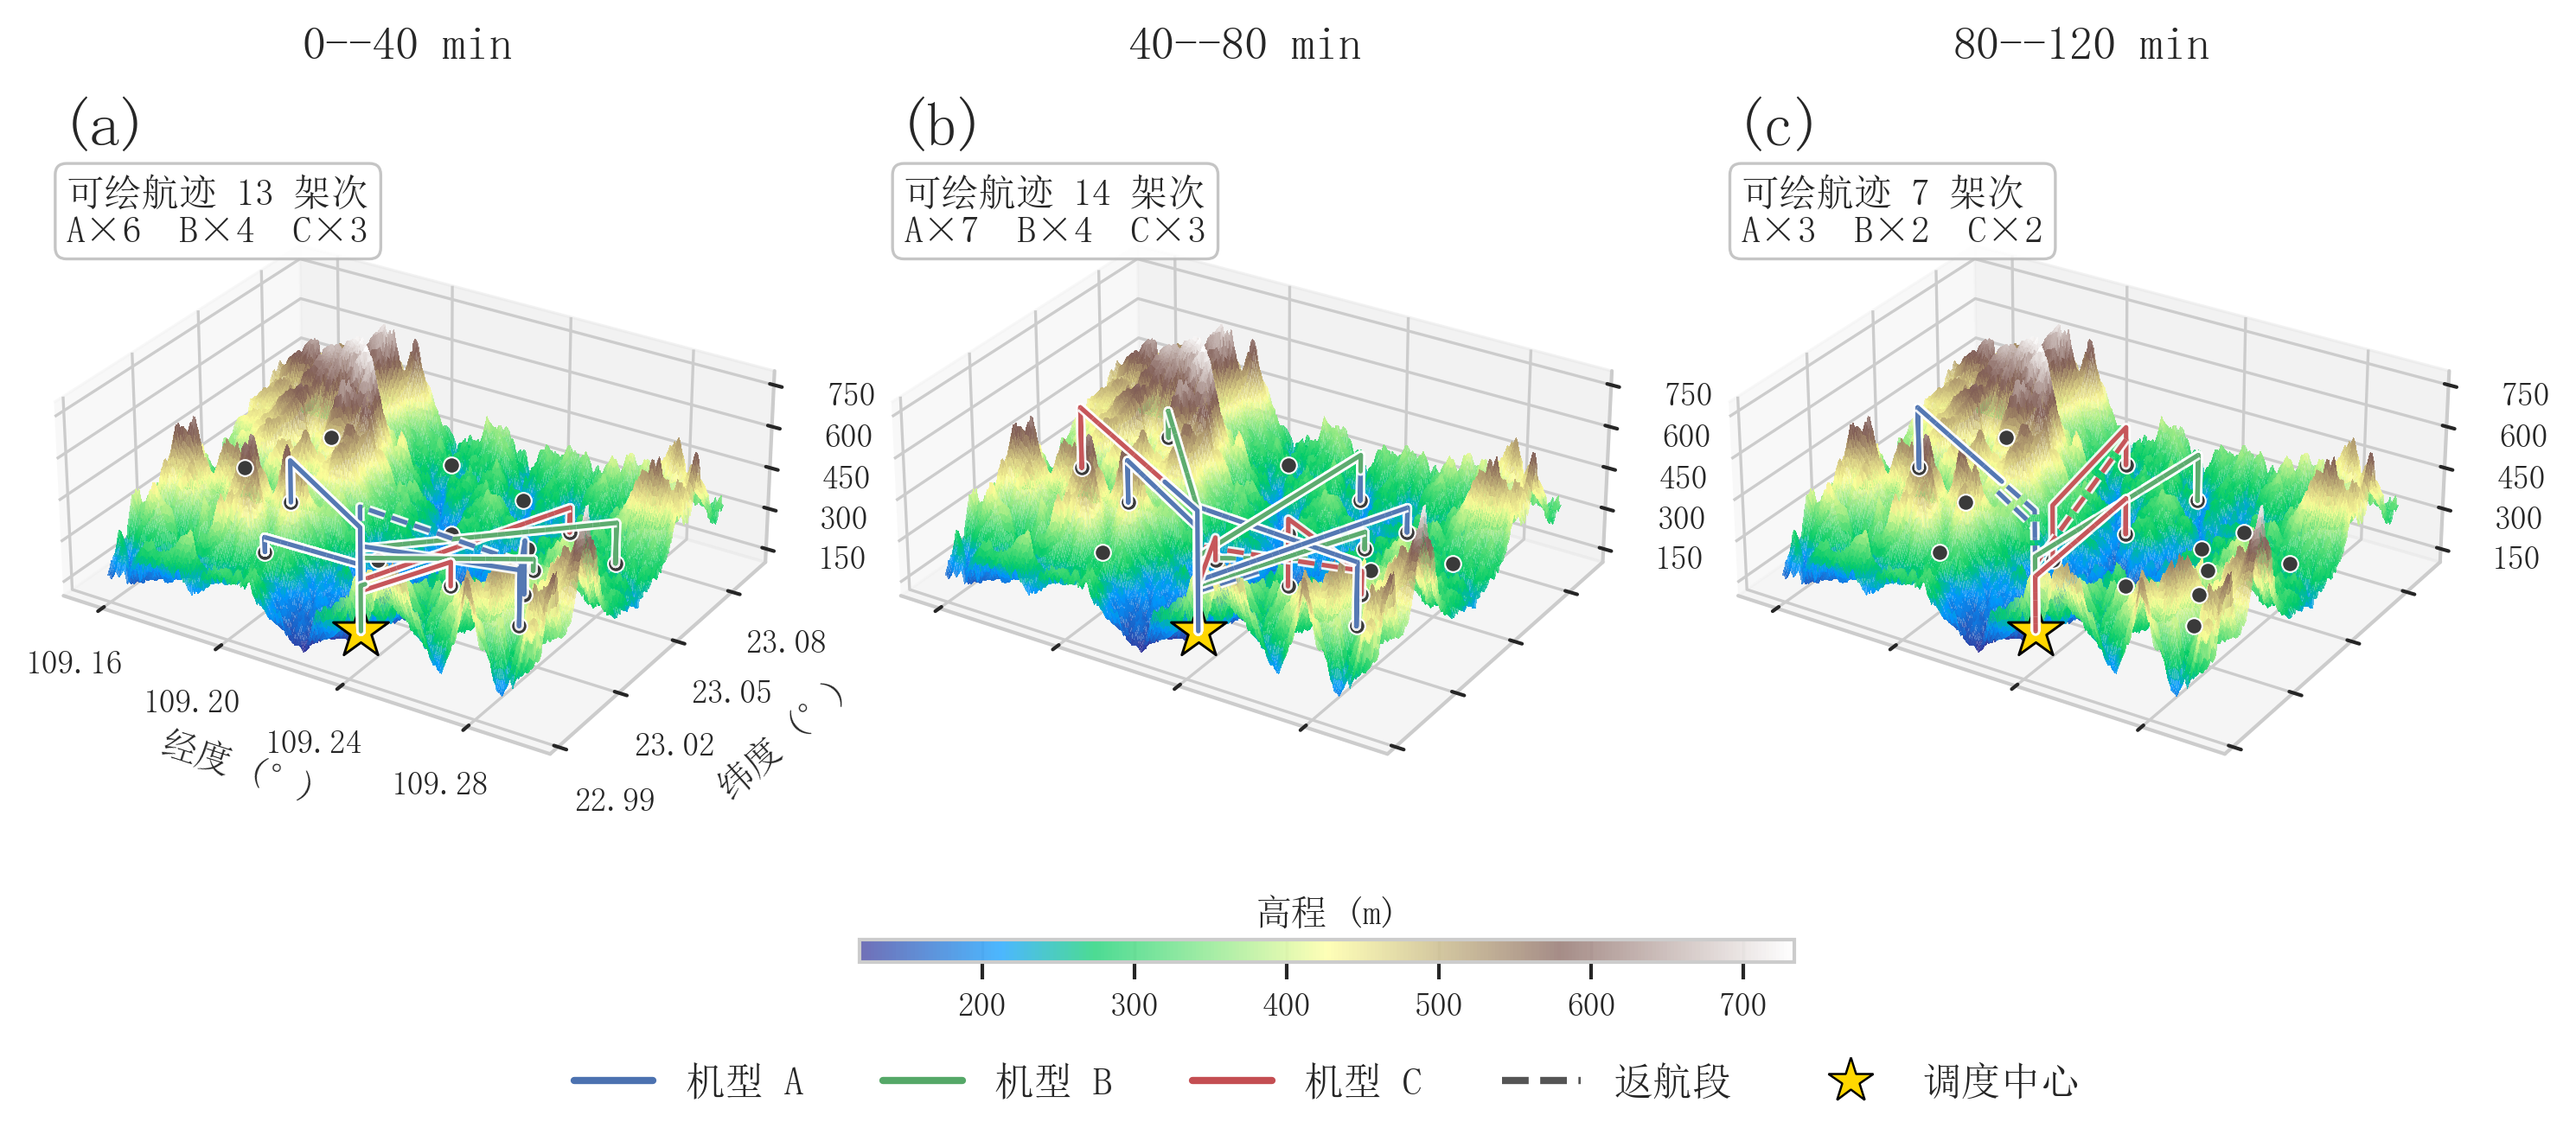
\includegraphics[width=0.95\textwidth]{figures/fig_q2_traj_evolution.png}
	\caption{问题二运输轨迹的分时段演化}
	\label{fig:q2-traj}
\end{figure}

图~\ref{fig:q2-traj}把同样这 24 个架次按 0--40、40--80、80--120\,min 三段切开，各段的航迹叠在同一片三维地形之上：颜色对应机型，实线为投送段、同色虚线为投送完成后的返航段，金色星标是调度中心。三个时段中能画出航迹的架次依次为 13、14、7，三者之和大于 24，是因为单个架次的耗时跨越 40\,min 的分段边界时会被相邻两段各记一次；首段是 13 而非 16，是因为 T14、T15、T16 虽在 40\,min 之前已开始地面准备，其在首段内仍处地面、不足两个采样点，爬升与巡航都落在第二段——图上取的是「该段内确有航迹可画」这一口径，与图中所见一致。第三段只剩 7 条航迹，而其中最后一个返航时刻正是 $6506.1$\,s 的完工时刻（$108.4$\,min）：本方案的收尾阶段在飞机队已相当稀疏，完工时刻落在跨区 C 型架次 T21（S011$\to$S008）的返航上；这与 6.2 节的判断一致——按能耗最小选型会把完工时刻压到只占机队四分之一的 C 型机上，派工优先级 $\pi$ 正是为化解这一瓶颈而引入的。最后是读数口径：纵轴作了约 $7.8$ 倍的垂向夸张（水平实距约 $14.2$\,km $\times$ $10.9$\,km，而窗口内高程幅度不足 $0.9$\,km），故图中的陡缓不能按视觉斜率判读；水平两轴为真实经纬度，服务区点位按其作业海拔（地面以上 30\,m）绘制。
\begin{table}[htbp]
	\caption{问题二的 $\varepsilon$-约束扫描结果}
	\label{tab:q2-pareto}
	\centering
	\small
	\setlength{\tabcolsep}{4.5pt}
	\begin{tabular}{ccccccc}
		\toprule
		架次上限 $K$ & 实际架次 & 能耗（kWh） & 完成时间（h） & 加权时延 & 硬违约 & 非支配 \\
		\midrule
		20 & 20 & 67.033 & 2.53 & 0 & 0 & 是 \\
		22 & 22 & 69.341 & 1.91 & 0 & 0 & 是 \\
		\textbf{25} & \textbf{24} & \textbf{69.316} & \textbf{1.81} & \textbf{0} & \textbf{0} & \textbf{是} \\
		30 & 24 & 69.342 & 1.81 & 0 & 0 & 否 \\
		\bottomrule
	\end{tabular}
\end{table}

表~\ref{tab:q2-pareto}的最右一列按（实际架次、能耗、完成时间、加权时延）四个维度对四档两两比较后逐档标出：只有 $K\le30$ 一档被支配——它与 $K\le25$ 一档的实际架次相同（均为 24 架）、完成时间也相同（$6506.1$\,s），而能耗更高（69.342 对 69.316\,kWh），故被 $K\le25$ 一档严格占优，本文不把它列为前沿档。其余三档互不支配，共同构成四维非支配前沿；四个档位的硬违约均为 $0$。需要说明的是，扫描本身仍然如实保留被支配档的原始记录（\texttt{results/q2\_scan.csv}），标“否”只表示它不进入前沿，不表示该档不可行。

前沿上呈现出一个方向明确但代价不菲的权衡：把架次上限从 20 放宽到 25，完成时间由 $9114.4$\,s 缩至 $6506.1$\,s（$-28.6\%$），代价是架次由 20 增至 24（$+20\%$）、能耗由 67.033 增至 69.316\,kWh（$+3.4\%$）。值得注意的是 $K\le20$ 一档的位置：它是四档中\textbf{能耗最低}（$67.033$\,kWh，比推荐档低 $3.3\%$）、\textbf{架次最少}（20 个）的一档，但完成时间最长（$9114.4$\,s，比推荐档长 $40.1\%$）。三档的加权时延都已为 $0$，无法再靠放宽架次换取。按式~\eqref{eq:q2-key} 的字典序，四档的加权时延并列于 $0$，比较进入第二层「完成时间」，$K\le25$ 档胜出；\textbf{若把能耗置于完成时间之前，则会选中 $K\le20$ 档}。本文取前者，因为题目把「及时性」排在能耗之前，而完成时间是本文口径下对及时性最直接的度量；这一取舍的依据是题目次序，不是「$K\le25$ 档全面更优」——它在能耗与架次上都劣于 $K\le20$ 档。

\textbf{消融实验。}由于派工顺序本身就能带来可观改进，若不做消融，很容易把“顺序的功劳”误记到“组批搜索”头上。故本文固定同一初始解与同一迭代预算（$3\,000$ 轮、单种子），分别关闭顺序搜索与组批搜索；第五行保持与④完全相同的协议（同轮数、同种子、同样放开架次数上限），只把求解引擎换成 6.2 节的三层移植实现，用来把“替换算法”的收益与“打开某个开关”的收益分开。结果如表~\ref{tab:q2-ablation}所示。

\begin{table}[htbp]
	\caption{ALNS 消融实验}
	\label{tab:q2-ablation}
	\centering
	\small
	\begin{tabular}{lccccc}
		\toprule
		配置 & 架次数 & 能耗（kWh） & 完成时间（s） & 加权时延 & 硬违约 \\
		\midrule
		① 基线（FFD 组批 + 紧迫度派工） & 25 & 84.779 & 14\,367.2 & 743\,943 & 0 \\
		② 仅顺序（组批冻结） & 25 & 78.293 & 9\,790.4 & 29\,526 & 0 \\
		③ ALNS（派工顺序固定） & 26 & 73.526 & 7\,235.7 & 0 & 0 \\
		④ ALNS 全量（组批 + 顺序） & 32 & 89.394 & 9\,447.7 & 51\,008 & 0 \\
		⑤ 三层全移（v2 引擎） & 28 & 82.042 & 7\,376.4 & 7\,245 & 0 \\
		\bottomrule
	\end{tabular}
\end{table}

由表~\ref{tab:q2-ablation}可得三点：其一，仅调整派工顺序（②）就把完成时间从 $14\,367.2$\,s 压到 $9\,790.4$\,s（$-31.9\%$）、加权时延降低 $96.0\%$（$743\,943\to29\,526$），说明顺序确实是本题的一等决策变量；其二，进一步开放组批搜索（③）把完成时间压到 $7\,235.7$\,s、能耗降到 $73.526$\,kWh、加权时延归零，是四个“受限配置”中最好的一行；其三，\textbf{④ 与 ⑤ 在放开架次数上限后同时退化}——④ 升到 32 架次、$89.394$\,kWh（比基线高 $5.4\%$）、时延 $51\,008$，⑤ 升到 28 架次、$82.042$\,kWh、时延 $7\,245$，两行的四项指标都不如架次受限的 ③，尽管它们的解空间严格更大。这不是模型矛盾，而是固定迭代预算下的搜索质量问题：推荐解（24 架次、$6506.1$\,s）要求先把架次数压下来，而放开上限后搜索更容易停在“多架次、长完工”的局部解。\textbf{⑤ 对 ④ 的四项全面改进}（架次 28 对 32、能耗 82.042 对 89.394\,kWh、完成时间 $7\,376.4$ 对 $9\,447.7$\,s、时延 $7\,245$ 对 $51\,008$）说明三层移植本身确实有效，只是不足以弥补放开上限带来的退化。本文如实报告这一现象，不将其粉饰为“全量搜索更优”。

推荐方案取 $\varepsilon$-约束扫描中 $K\le25$ 档的可行解（24 架次、69.316\,kWh、$6506.1$\,s、加权时延 0）。把它与消融五行逐维比较：它在\textbf{架次数}（24 对 25 / 25 / 26 / 32 / 28）、\textbf{能耗}（69.316 对 84.779 / 78.293 / 73.526 / 89.394 / 82.042\,kWh）、\textbf{完成时间}（$6506.1$ 对 $14\,367.2$ / $9\,790.4$ / $7\,235.7$ / $9\,447.7$ / $7\,376.4$\,s）与\textbf{加权时延}（0 对 $743\,943$ / $29\,526$ / 0 / $51\,008$ / $7\,245$）四项上\textbf{均不差且至少一项严格更优}，即对全部五个配置构成\textbf{全面占优}。但这一比较的边界必须讲清楚：消融各行统一取 $3\,000$ 轮、单种子、同一初始解，而推荐解来自 $5$ 种子 $\times$ $3\,500$ 轮 $\times$ $4$ 档的扫描再加逐档定型，预算远大于消融各行。故它说明的是“\textbf{本文的完整求解链优于任一单项配置}”，\textbf{不能}读作“算法在同等预算下全面更优”。

\subsection{小规模精确验证}

ALNS 是启发式，其解的质量需要独立证据。本文设计两层小规模精确验证，验证逻辑与适用范围均如实标注。

\textbf{Layer A（分区层，无路径简化）。}取 3 个服务区构成小算例，穷举全部架次模式（列生成）后用两层字典序集合划分整数规划求精确最优：先最小化架次数，再在最小架次下最小化能耗。这里必须说明正确性的理由不是“架次最多访问 3 个服务区”——该命题为假，实测存在能量可行的 5 服务区架次——而是：算例只含 3 个服务区时，任何架次的区域集合必然是该 3 区的子集，故 3 个区的 6 个排列即全部可能路径，区域集合与访问顺序被同时穷举。为保证对比有效，ALNS 在该算例上以同一服务区子集运行。

\begin{table}[htbp]
	\caption{ALNS 与精确解的最优性间隙}
	\label{tab:q2-exact}
	\centering
	\footnotesize
	\setlength{\tabcolsep}{4pt}
	\begin{tabular}{llcccc}
		\toprule
		层级 & 算例 & 模型规模 & 精确模型 & 启发式对照 & 精确相对启发式 \\
		\midrule
		A & S013+S014+S015（9 箱） & 160 列 & 2 架次 / 7.3226 & ALNS 2 / 7.3226 & $0$ \\
		A & S009+S010+S011（9 箱） & 1\,068 列 & 2 架次 / 6.3665 & ALNS 2 / 6.3665 & $0$ \\
		A & S002+S009+S010（14 箱） & 6\,262 列 & 3 架次 / 12.9433 & ALNS 3 / 12.9433 & $0$ \\
		\addlinespace
		B1 & 固定指派·最短完工 & 118 二元 & 14\,029.8\,s\dag & 贪心 14\,367.2\,s & $+2.40\%$ \\
		B1$'$ & 固定指派·加权时延 & 118 二元 & 703\,470.6\ddag & 贪心 743\,943.2 & $+5.75\%$ \\
		B2 & 自由指派·最短完工 & 630 二元 & 13\,565.2\,s\S & 贪心 14\,367.2\,s & 见注~\S \\
		\bottomrule
	\end{tabular}

	\vspace{2pt}
	{\footnotesize \dag\ 已证最优，但该解\textbf{违反 8 项硬时限}，只作下界参考；\quad
	\ddag\ 已证最优，加权时延口径，硬违约 $0$；\quad
	\S\ 90\,s 时限内\textbf{未证最优}（上下界间隙 $65.77\%$），此为该时刻的可行上界；该上界虽比贪心排程\textbf{短 $5.58\%$}，但它\textbf{违反 9 项硬时限}，不构成可行方案，故该行不给出“精确相对启发式”的比值。}
\end{table}

Layer A 的三个算例最优性间隙全部为 $0$，且都在 1\,000 次迭代内收敛。值得强调的是，这层验证并非装饰：最初的 ALNS 在三个算例上跨 3 个随机种子、12\,000 次迭代都\textbf{系统性停在 3 架次}（非最优），排查后确认根因正是上文所述的代理代价缺陷——B 型无人机仅 2 架，而最优解需要“把 S013 与 S014 合并为一架 C 型架次以腾出一架 B 给 S015”，该动作在代理代价下永远显示为“更贵”。补入成组修复算子后间隙归零。这正是“小规模精确解验证启发式”的实际价值：它抓到了一个贪心代理看不见的机队瓶颈型协同。

\textbf{适用范围必须声明}：Layer A 的三个算例均只含 3 个服务区，8 架无人机对至多 9 个架次，\textbf{机队资源竞争几乎不存在}，故它验证的是组批、能耗与路径逻辑的正确性，\textbf{不能}外推为“全局资源拥塞情形下已证最优”。

\textbf{Layer B（时序层，big-M 析取 MILP）。}固定贪心方案的机型指派，只放开架次的执行无人机、共享电池与开始时刻，用 big-M 析取约束表达“同一无人机/电池的占用区间不重叠”\cite{grossmann2011generalized}。$M$ 的取值必须满足 $M\ge UB+\max\tau$（$\max\tau$ 为全部充电操作中最长的充电时长；此处不引入充电资源的下标，以免与货箱编号 $c$ 撞车），其中 $UB$ 由一份\textbf{计入充电占用的完全串行排程}给出（本文实测：取 $M=UB$ 会漏掉充电等待而制造假不可行，这个坑踩过）；为保证该界不截掉可行解，还对贪心排程本身做了暖可行性回放，实测 $M=94\,881.2$\,s、贪心完工距上界尚有 $80\,514$\,s 余量。两个固定指派变体分别以最短完工与最小加权时延为目标，分别在 3.4\,s 与 2.3\,s 内证到最优（均含列与约束构建时间），且解回放后无资源重叠。第三行的自由指派变体在 90\,s 时限内\textbf{未证到最优}，本文按实测状态如实记为“超时但有可行解”，不记为不可行、也不记为最优。

两个层次得到的间隙与劣化幅度并排呈现于图~\ref{fig:q2-exact}。

\begin{figure}[htbp]
	\centering
	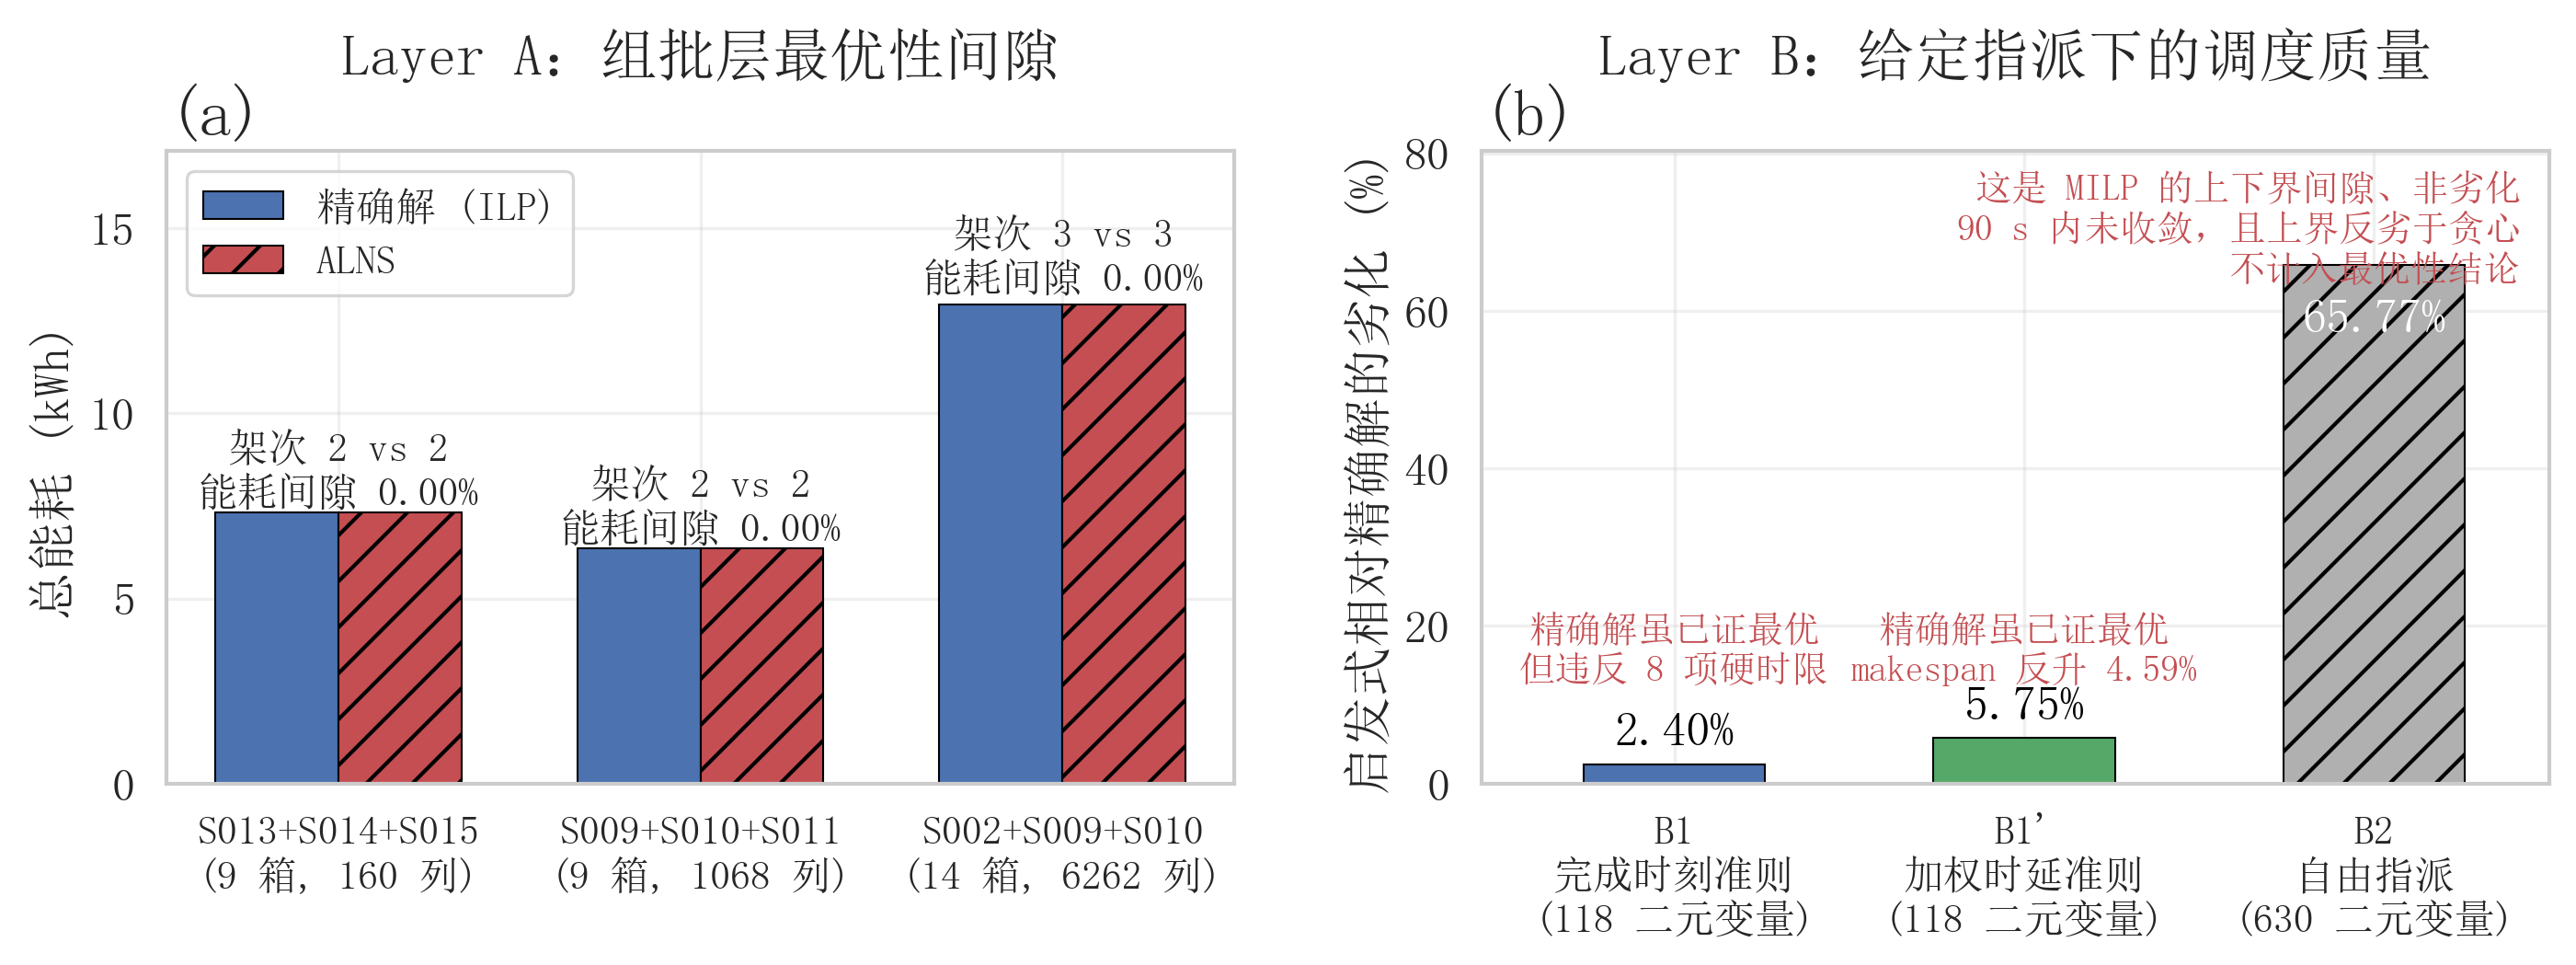
\includegraphics[width=0.95\textwidth]{figures/fig_q2_exact.png}
	\caption{ALNS 相对精确解的劣化与间隙}
	\label{fig:q2-exact}
\end{figure}

图~\ref{fig:q2-exact}把表~\ref{tab:q2-exact}的间隙按口径并排呈现。B1 与 B1$'$ 给出的是“给定贪心指派，贪心调度已接近最优”的\textbf{证书}：最短完工口径下贪心仅比最优差 $2.40\%$（$14\,367.2$ 对 $14\,029.8$\,s），加权时延口径下仅差 $5.75\%$（$743\,943.2$ 对 $703\,470.6$）；而两者互相印证了“完成时间与时延不可兼得”——B1 的最优解 makespan 最短，但其\textbf{违反 8 项硬时限}（故不作为可行方案，仅作下界参考）；B1$'$ 的最优解硬违约数为 0，但其 makespan 为 15\,026.7\,s，比贪心还差 $4.59\%$。B2 放开了物理指派，变量数由 118 增至 630，求解 90\,s 后上下界间隙仍有 $65.77\%$。该时刻的可行上界为 13\,565.2\,s，比贪心排程（14\,367.2\,s）还短 $5.58\%$——但它\textbf{违反 9 项硬时限}，与 B1 一样只是「放松问题的一个下界方向」，不是可交付的方案；而 65.77\% 的间隙也说明这个上界离真正的最优还差得远。故本文\textbf{不把 B2 计入任何最优性结论}，也不引用其目标值作为对照——它只说明「自由指派层的精确求解规模已超出 90\,s 能处理的范围」，这一局限已列入第 10 章的模型缺点。

最后说明货箱到架次的映射关系。图~\ref{fig:q2-flow}给出推荐方案中“服务区—架次—机型”的三层流向，可以看出流量在 C 型与 B 型之间的分配与问题一的结论一致：重载服务区走 C 型，轻载服务区走 B 型，而 A 型主要承担紧急货箱的轻载快投。

\begin{figure}[htbp]
	\centering
	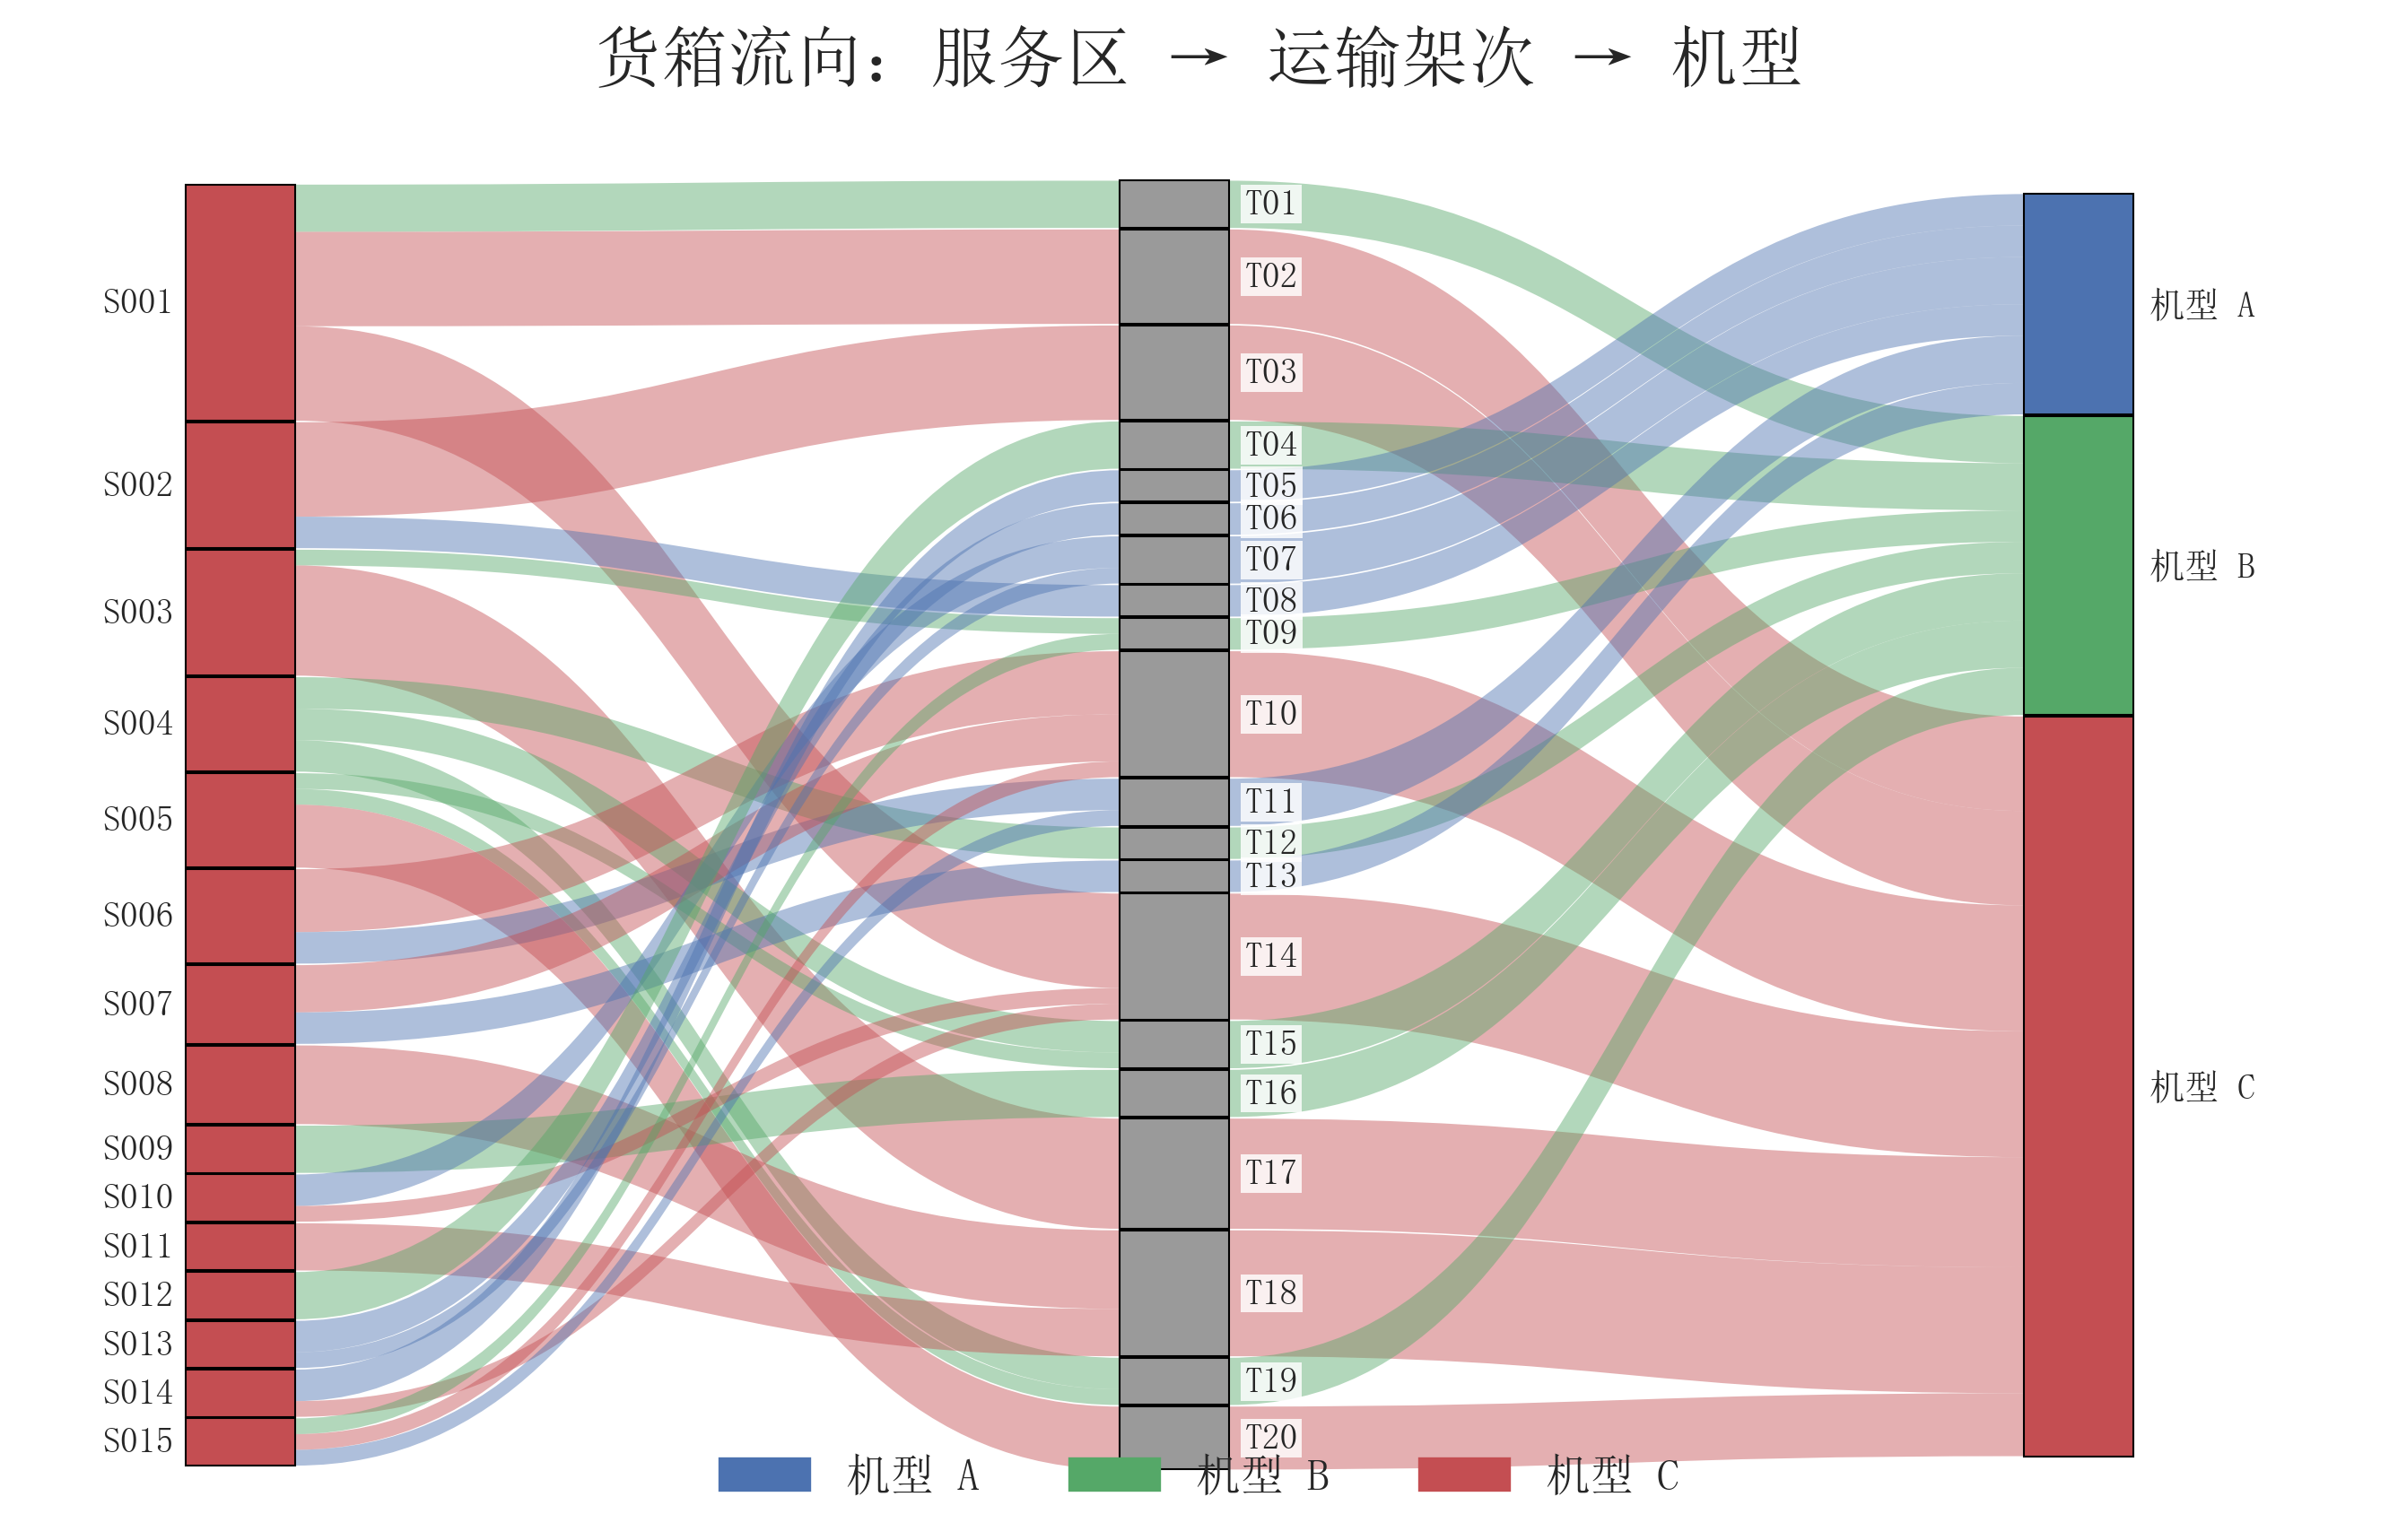
\includegraphics[width=0.95\textwidth]{figures/fig_q2_flow.png}
	\caption{服务区—架次—机型的三层流向}
	\label{fig:q2-flow}
\end{figure}

\textbf{本节向问题三输送什么。}问题二的产出是一张完整的运输时刻表：24 个架次各自的机型、访问顺序与开始时刻，80 个货箱各自的承运架次与交付时刻。问题三直接站在这张表上——它的输入校验要求错峰表 \texttt{q3\_stagger.csv} 的「原开始时刻」一列恒等于问题二架次表的「开始时刻」（第 \ref{sec:feasib-deliv} 节），也就是说不允许下游悄悄换一张时刻表再声称「在问题二基础上改进」。承接的方式则是有选择的：问题三\textbf{保留组批与航线不变}（哪个货箱在哪架次、架次访问哪些服务区都不重排），只把开始时刻当作可调量，再在其上叠加中继侧的决策（悬停站的坐标与离地高度、中继架次的派发与能源组件分配）。这一层切分是本文为控制搜索规模而作的设计选择，不是题目的可行域要求：题目并未禁止相对问题二基线提前，提前是否可行只取决于释放、无人机与电池的就绪时刻以及硬时限。代价则很明确——「靠改组批、改航线或提前腾出通信余量」这部分解空间被放弃了，该局限列入第 10 章。
         % 六、问题二
\section{问题三：通信约束下的运输与中继联合调度}

题面把「连续通信」与货箱时限、载荷与能量、资源可用性并列为\textbf{约束}，即运输无人机在爬升、巡航、下降与投送的全过程都必须保持与调度中心的可通信状态。问题二的调度只优化了运输本身，沿其轨迹逐时刻判定直连链路可得如下事实：\textbf{71.67\% 的时间可直连，其余 28.33\% 处于通信盲区}。也就是说，若把中继保障作为事后补救，问题二的方案在通信连续性上根本不可行。本节把运输开始时刻、中继站选址与悬停高度、中继架次调度纳入同一个联合优化模型，并以“集合覆盖整数规划选站＋沿资源链级联错峰＋就绪性修复环”分层求解。

\subsection{联合优化模型}

\textbf{决策变量}（三层）：
\begin{itemize}
	\item 运输层：延续问题二的货箱组批与路线，把架次 $p$ 的开始时刻 $s_p$ 升为决策变量（即错峰量 $\Delta_p=s_p-s_p^{0}$）；
	\item 通信层：悬停站选址二元变量 $y_r\in\{0,1\}$，候选点 $r=(\lambda_r,\varphi_r,h_r)$ 同时含水平坐标与悬停离地高度 $h_r\in\{50,100,150,200,250,300\}$\,m；
	\item 调度层：中继架次的派发顺序与各架次的起飞、建链、服务、返航时刻。
\end{itemize}

\textbf{约束}：① 通信连续性 $C_p(t)=1,\ \forall p,\forall t$；② 问题二的全部约束在错峰后仍须成立（货箱硬时限、载质量与体积、返航能量余量、无人机与共享电池周转）；③ 中继侧的中继无人机与能源组件周转；④ 建链完成时刻不得晚于所服务失效区间的结束时刻。

\textbf{目标}为两层字典序：先\textbf{最小化通信中断时间}（须为 0），再在中断为 0 的前提下最小化悬停站数与中继总能耗。把「连续通信」写成必须归零的硬指标而非加权项，是因为题面已把它列为约束——加权只会把它降格为可交易项。

\subsection{直连失效区间与通信盲区}

对问题二推荐方案的每个运输架次，沿其三维轨迹（爬升、巡航、悬停交接、下降）按 $\Delta t$ 采样，逐点按式~\eqref{eq:pathloss} 计算路径损耗，并按第 \ref{sec:link-model} 节的双向链路门限判据判定直连可用性（含地形遮挡）。判定的一个有用性质是：\textbf{直连可用性只取决于轨迹的几何形状，与绝对时刻无关}，故错峰平移不会改变直连时间占比——这也是后文三组对照中直连占比恒为 $71.67\%$ 的原因。

在联合优化后的排班上，24 个运输架次中共有 19 个出现连续失效，形成 \textbf{19 个失效区间}（编号 G01--G19，逐区间明细见 \texttt{q3\_intervals.csv}），其时间之和占全部飞行时间的 $28.33\%$。区间在空间上分为若干片互不相连的地形阴影区，需由不同位置的悬停站分别覆盖，如图~\ref{fig:q3-relay}中的红色散点所示。

\begin{figure}[htbp]
	\centering
	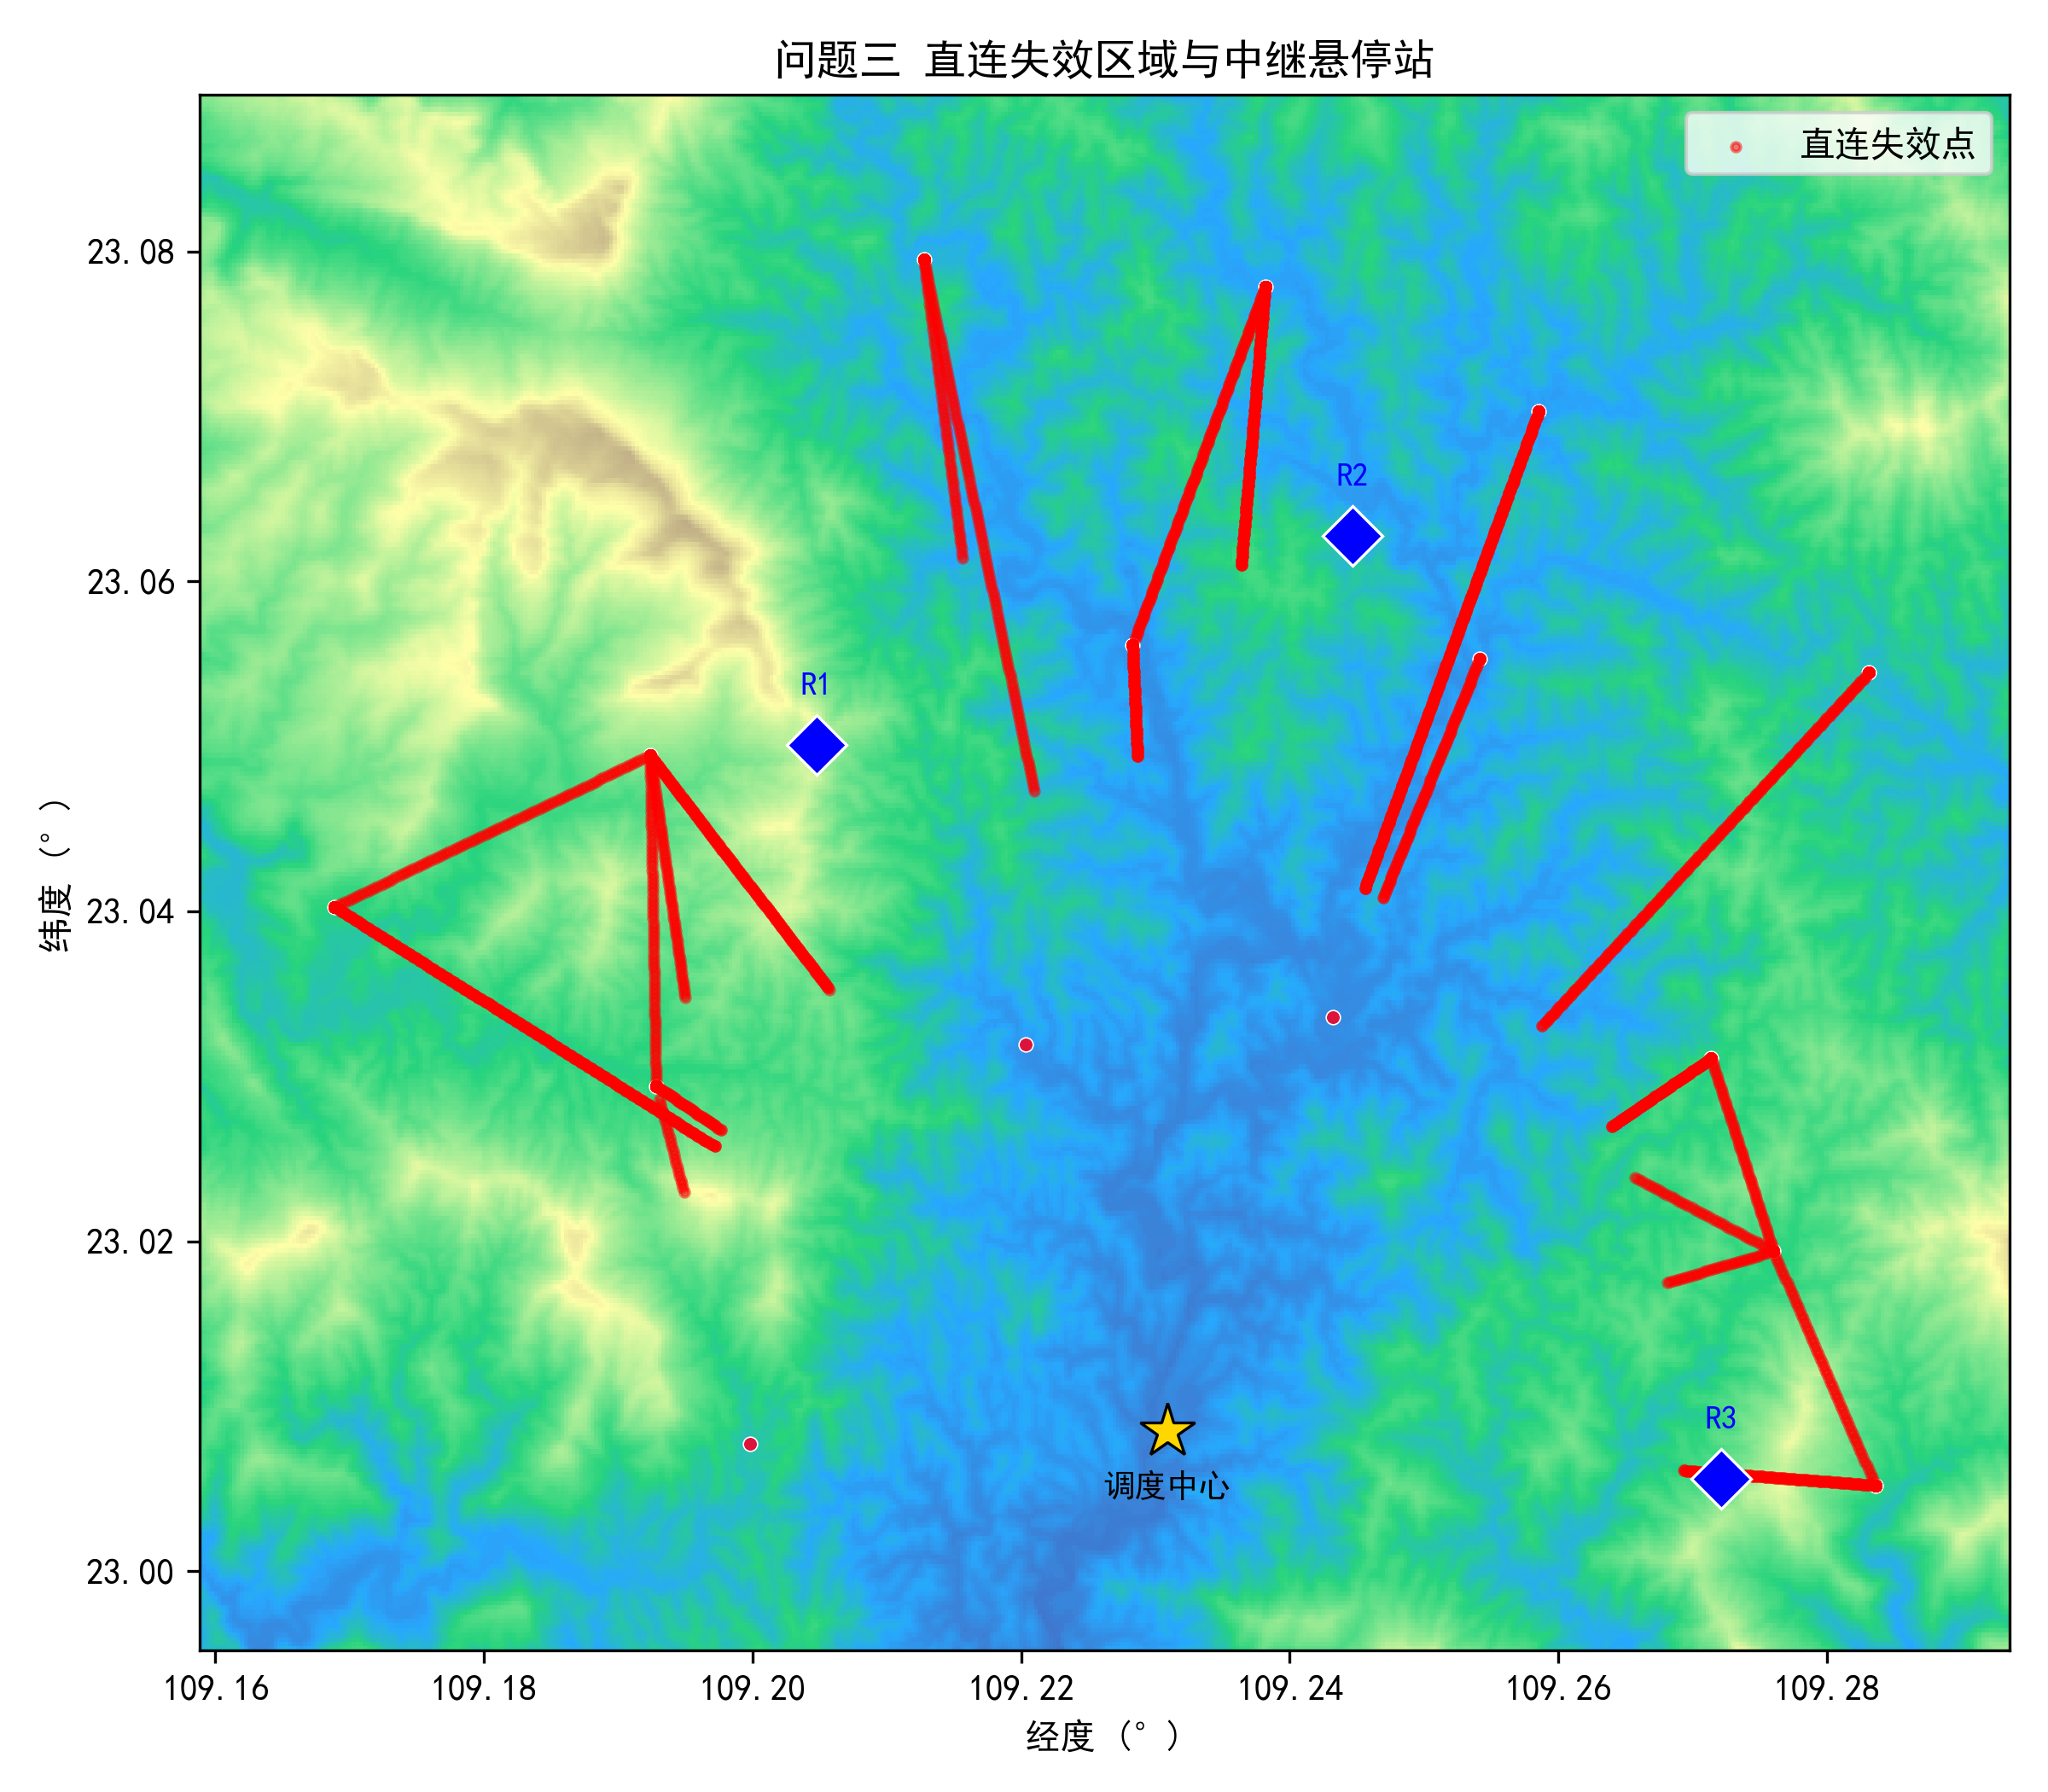
\includegraphics[width=0.82\textwidth]{figures/fig_q3_relay.png}
	\caption{直连失效区域与中继悬停站}
	\label{fig:q3-relay}
\end{figure}

\subsection{三维悬停站的集合覆盖选址}

候选悬停点由失效点包围盒内步长 1200\,m 的水平网格（$11\times8$）与 6 档离地高度交叉生成\cite{elnabty2022survey}，共 \textbf{342 个}，保留其中能与 G01 建立回传链路者。对候选点 $r$ 与失效区间 $j$ 预计算覆盖系数 $a_{jr}\in\{0,1\}$：$a_{jr}=1$ 当且仅当 $r$ 在 $h_r$ 高度上能对区间 $j$ 所属运输架次的\textbf{全部}轨迹采样点建立接入链路。本算例每个区间的可覆盖站数为 22--204 个，不存在无站可覆盖的区间。选站即求解集合覆盖问题\cite{church1976theoretical}
\begin{equation}
	\min \sum_{r} y_r \quad \text{s.t.}\quad \sum_{r} a_{jr}\,y_r \ge 1,\ \ \forall j,
	\label{eq:setcover}
\end{equation}
再以两层字典序求解：先最小化站数，再在最小站数下最小化中继总能耗。求解过程中先以粗步长（每 5 个采样点取 1）构造覆盖矩阵以免假负例，随后对入选的 $(j,r)$ 对做\textbf{全密度复核}，剔除实际覆盖不完全的列并重解，构成列生成式的修复环。最后用坐标下降法对 $({\rm lon},{\rm lat},h)$ 做连续局部微调，最大化该站对最不利采样点的接入裕量。

集合覆盖先给出 \textbf{3 个悬停站}，几何上已覆盖全部 19 个区间。但「几何上覆盖」不等于「届时守得住」：中继机只有 2 架，某些区间在其被覆盖的站上等不到中继机到位。第 \ref{sec:q3-repair} 节的\textbf{换站修复}为此改换部分区间的归属站，另引入 2 个站，最终方案共 \textbf{5 个悬停站}（表~\ref{tab:q3-stations}）。

\begin{table}[htbp]
	\caption{中继悬停站选址结果}
	\label{tab:q3-stations}
	\centering
	\small
	\begin{tabular}{cccccc}
		\toprule
		编号 & 经度（$^\circ$） & 纬度（$^\circ$） & 地面高程（m） & 离地高度（m） & 保障区间数 \\
		\midrule
		S01 & 109.1916 & 23.0284 & 359.03 & 100 & 5 \\
		S02 & 109.2262 & 23.0371 & 211.09 & 300 & 3 \\
		S03 & 109.2378 & 23.0689 & 245.42 & 200 & 4 \\
		S04 & 109.2492 & 23.0583 & 252.18 & 300 & 1 \\
		S05 & 109.2721 & 23.0056 & 407.44 & 190 & 6 \\
		\bottomrule
	\end{tabular}
\end{table}

值得注意的是，五站的离地高度为 $100$、$300$、$200$、$300$、$190$\,m：\textbf{三站落在中间档、两站顶到题给上限 $300$\,m}。这说明悬停高度是一个真正起作用的决策变量，但它的作用是\textbf{非单调}的——选站的字典序目标是最小化站数、再最小化中继总能耗，而站址与离地高度的连续精化准则是最大化该站对所辖区间最不利采样点的接入裕量（同时保持回传可用、不超高度上限）。当地形阴影较深时，抬高到上限是唯一能建立接入的选择；当阴影较浅时，中间档即可满足裕量，无须付出额外爬升。故不能笼统地说「最优解不会顶到上限」，只能说\textbf{是否顶到上限由该片阴影区的地形决定}。

\subsection{中继架次调度与运输错峰}
\label{sec:q3-repair}

\textbf{服务时段合并。}一个悬停站在一段时间内往往要连续保障多个运输架次的失效区间，若逐段派发会产生大量固定开销（起飞准备、爬升建链、返航周转）。故\textbf{只按悬停站分组}，把同一站上间隔不超过 $900$\,s 的失效区间合并为一个中继服务任务，并限制单个任务跨度不超过 $3600$\,s；合并\textbf{不要求这些区间来自同一运输架次}，因为中继机在合并窗口内持续悬停，与它此刻保障的是哪一架运输机无关，跨架次合并正是省下整次出动的主要来源。本算例的 19 段失效区间经合并后只需 7 次悬停服务。

\textbf{中继架次能耗。}每个中继架次 $k$ 的能耗按题给口径由水平巡航、爬升附加与悬停通信三部分组成：
\begin{equation}
	E^{R}_{k}=P^{c}_{R}\frac{d_{k}}{v^{c}_{R}}\frac{1}{3600}
	+\frac{1}{3.6\times10^{6}}\cdot\frac{m^{\mathrm{TO}}_{R}\,g\,h^{+}_{k}}{\eta^{\uparrow}_{R}}
	+\big(P^{\mathrm{hover}}_{R}+P^{\mathrm{comm}}_{R}\big)\frac{t^{\mathrm{svc}}_{k}}{3600},
	\label{eq:relay-energy}
\end{equation}
其中 $m^{\mathrm{TO}}_{R}$ 为计划起飞总质量（悬停与爬升均按此质量计），$t^{\mathrm{svc}}_{k}$ 为悬停服务时长；三项分别由 kW$\cdot$s 与 J 折算为 kWh 后求和。每个中继架次同样须满足返航电量约束 $E^{R}_{k}\le(1-\rho_{R})E^{\mathrm{use}}_{R}$。

\textbf{弃飞规则。}若某中继架次飞抵悬停点并完成建链的时刻已晚于所服务失效区间的结束时刻，则该架次提供不了任何通信保障。这类架次不能「照飞不误」——它同样占用一架中继无人机和一组能源组件，会把后续本可按时到达的架次一并顶迟到，形成级联迟到。故调度规则中显式加入一条：\textbf{建链时刻晚于区间结束时放弃派发该架次}，弃飞数在结果中如实报告。

\textbf{运输错峰。}在保持问题二组批与路线不变的前提下，把各运输架次的开始时刻后移，使同一时刻需要中继保障的\textbf{不同悬停站}数不超过 2（题给的中继无人机数）。错峰不是简单的削峰：单个架次的后移会被同一条无人机/电池资源链上的下一架次顶回，因此本文沿资源链\textbf{级联传播}推迟量，而非逐架次试探。其后还有两级修复：\textbf{就绪性修复}把「中继届时尚未到位」的区间所属运输架次沿资源链后移，直到中继建链完成时刻不晚于区间起点（推迟上限受货箱硬时限的松弛量约束）；\textbf{换站修复}则在就绪性修复已顶死硬时限时，把区间改派给「中继届时真在位」的另一个站，补上集合覆盖看不见的时间维度。实测就绪性修复是推迟量的主要来源：最终 11 个被推迟架次中，多数架次的失效区间起点\textbf{恰好等于}其所绑中继架次的建链完成时刻（例如 T17 的 G12 起点 $8265.2$\,s 即 R06 的建链完成时刻、T23 的 G18 起点 $8575.6$\,s 即 R07 的建链完成时刻），说明这些架次的开始时刻是被中继链的到位时刻反推锁定的，而不是搜索取大的结果。

\subsection{问题二最优解的等价类：用第三问门禁择序}
\label{sec:q2-gate}

上述修复环解决的是「中继到位与运输到达的时序错配」。实施中还暴露出一个更靠上游的问题，本文如实记录并给出处置。

问题二的目标是「加权时延 $\to$ 完工时刻 $\to$ 能耗 $\to$ 架次数」的字典序，其中前两项与\textbf{每架无人机的总占用时长}有关，而与「同一架无人机上两个架次谁先飞」无关——调换先后不改变该机的总忙碌时间，故问题二的\textbf{最优解是一个等价类}，类内各元素的架次数、完工、能耗、加权时延可以逐位相同。但第三问的通信保障依赖\textbf{绝对时刻}：某个架次的失效区间若落在中继链的尾端，中继机返航周转赶不上，就会出现几百秒的迟建链。原方案正是如此：\textbf{195 个采样点（占全部时间的 $0.6688\%$）无人保障}，且这一缺口无法靠第三问单独消去——因为第三问只被允许改变各架次的开始时刻，而问题二的下游校验要求 \texttt{q3\_stagger.csv} 的「原开始时刻」恒等于问题二架次表的「开始时刻」（见第 \ref{sec:q3-check} 节），顺序必须由问题二本身给出。

故本文在问题二内部增加一层\textbf{确定性门禁}（\texttt{q2\_v2.relay\_feasible\_order}）：按无人机编号升序、下标升序枚举「同机两架次互换」的全部候选（本算例 24 个架次共 25 个候选），只保留使 \texttt{q2.evaluate} 报告的五项指标（架次数、完工、能耗、加权时延、硬违反）\textbf{逐位相等}的候选（实测 3 个），再把这 3 个候选与原序一并交给第三问，按第三问的字典序（无绑定区间数 $\to$ 缺口秒数 $\to$ 累计推迟量 $\to$ 联合完工 $\to$ 中继能耗）择优选出一条。由此：

\begin{itemize}
	\item \textbf{论文中报告的问题二数字一个都不变}——该层只改「谁先飞」，不改任何指标（代码中以断言 \texttt{assert \_relay\_metric\_key(m2) == base\_key} 把关）；
	\item \textbf{结果可复现}——候选枚举与排序都是确定性的，同种子跑两遍得到同一个顺序；
	\item \textbf{基线与候选一同参与比较}，故门禁不会把一个已经更好的顺序换差。
\end{itemize}

门禁最终选中无人机 U06 上派发序列第 6 位与第 8 位互换。问题二的五项指标逐位不变，而第三问的中断由 $0.6688\%$（195 个采样点）\textbf{降为 0}。这是一次\textbf{有代价的交换}，代价在第 \ref{sec:q3-cost} 节如实报告。

\subsection{求解结果与对照}

联合优化后共派发 \textbf{7 个中继架次}（R01--R07），由 2 架中继无人机分别飞 3 趟与 4 趟（R01$\to$\allowbreak R04$\to$\allowbreak R07 与 R02$\to$\allowbreak R03$\to$\allowbreak R05$\to$\allowbreak R06），占用 6 组能源组件（RC2 周转两次），弃飞 0 架次、迟建链 0 架次、未保障区间 0 个，中继总能耗 \textbf{4.493\,kWh}。19 个失效区间与中继架次的绑定关系完整给出（表~\ref{tab:q3-bind}节选），每站的保障区间数与表~\ref{tab:q3-stations}一致。

\begin{table}[htbp]
	\caption{运输架次—失效区间—中继架次绑定（节选）}
	\label{tab:q3-bind}
	\centering
	\small
	\begin{tabular}{cccccc}
		\toprule
		区间 & 运输架次 & 区间起点（s） & 区间终点（s） & 悬停站 & 中继架次 \\
		\midrule
		G01 & T04 & 2533.4 & 3479.5 & S02 & R03 \\
		G02 & T05 & 706.8 & 1232.8 & S05 & R01 \\
		G03 & T06 & 813.1 & 1235.0 & S01 & R02 \\
		G12 & T17 & 8265.2 & 8854.9 & S04 & R06 \\
		G13 & T18 & 5297.9 & 5948.1 & S03 & R05 \\
		G18 & T23 & 8575.6 & 9193.6 & S03 & R07 \\
		\bottomrule
	\end{tabular}
\end{table}

\textbf{三组口径对照。}为把「联合优化究竟带来了什么」讲清楚，本文按同一套时间积分口径（$\Delta t=1$\,s）给出三组对照（表~\ref{tab:relay-gap}）：\emph{无中继}即问题二的纯运输调度，\emph{序贯对照}为固定悬停高度 $300$\,m、贪心选站、不错峰、不做高度选择与连续精化的常规做法，\emph{联合优化}即本节方案。

\begin{table}[htbp]
	\caption{三种通信保障口径的对照（$\Delta t=1$\,s 时间积分）}
	\label{tab:relay-gap}
	\centering
	\small
	\setlength{\tabcolsep}{4pt}
	\begin{tabular}{lccccc}
		\toprule
		口径 & 直连占比 & 中继占比 & \textbf{中断占比} & 中继架次 & 中继能耗（kWh） \\
		\midrule
		无中继（问题二调度） & 71.67\% & 0 & \textbf{28.33\%} & 0 & 0 \\
		序贯对照 & 71.67\% & 24.22\% & \textbf{4.11\%} & 3 & 3.019 \\
		\textbf{联合优化} & 71.67\% & 28.33\% & \textbf{0.00\%} & 7 & 4.493 \\
		\bottomrule
	\end{tabular}
\end{table}

可见三点。其一，\textbf{中继不是锦上添花而是必需}：不做中继时运输全过程有超过四分之一的时间处于通信盲区，方案在题面约束下不可行。其二，把高度、站址、错峰纳入决策后，中断由序贯方案的 $4.11\%$ 归零，付出了 4 个额外中继架次与 $1.47$\,kWh 的能耗——序贯对照之所以只需 3 架次，正是因为它\emph{不管}剩余 $4.11\%$ 的盲区，两者的架次数不能直接相比。其三，直连占比在三组中完全一致，说明所有改善都来自中继侧与错峰的协同，而不是通过改变航线「绕开」阴影区。

图~\ref{fig:q3-timeline}以时序带的形式给出结论：上方为每个运输架次的通信状态（直连/中继/中断三色），下方为 7 个中继架次的占位窗口；可以看到全部架次带中\textbf{不存在中断色段}，且任一时刻占位的中继架次不超过 2 个，与题给的 2 架中继无人机容量相符。

\begin{figure}[htbp]
	\centering
	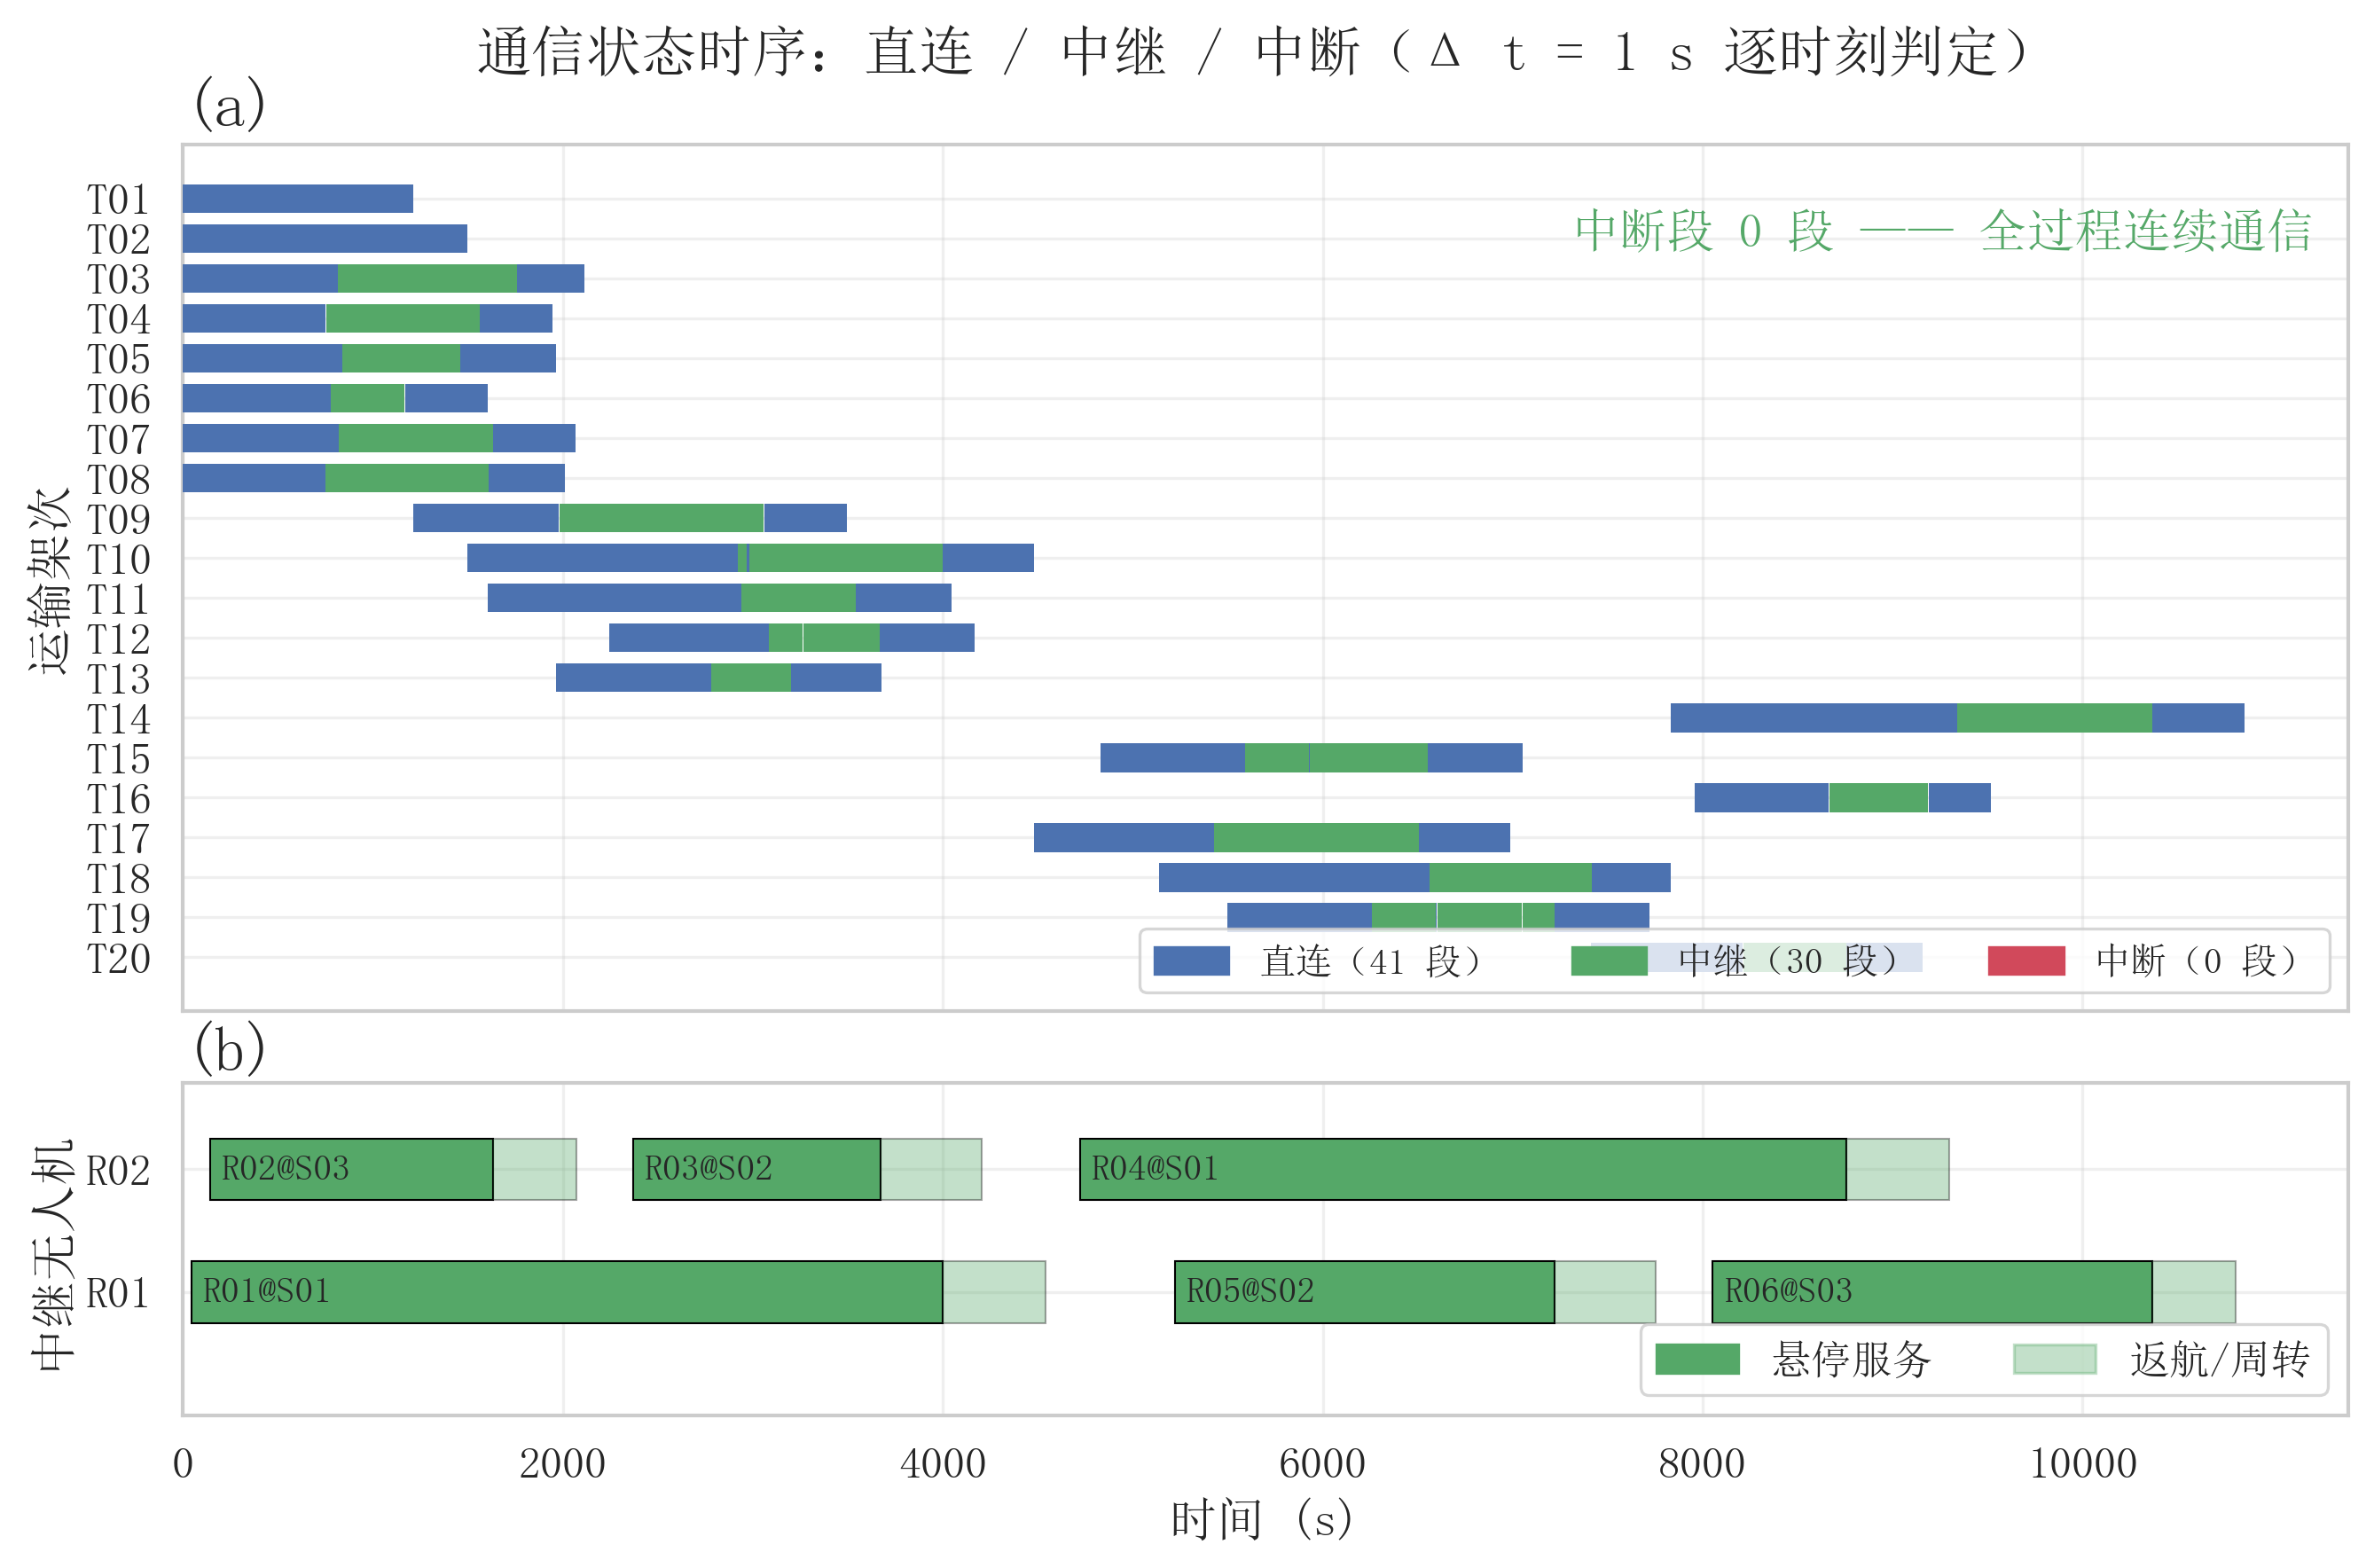
\includegraphics[width=0.95\textwidth]{figures/fig_q3_timeline.png}
	\caption{通信状态时序带与中继服务窗口}
	\label{fig:q3-timeline}
\end{figure}

图~\ref{fig:q3-analysis}给出中继侧的几何诊断：五个悬停站在地形上的三维位置、各站的接入裕量分布与覆盖区间数。五站中 S05 与 S01 承担的区间最多（6 个与 5 个），S03 覆盖 4 个，S02 覆盖 3 个，S04 只压住 1 个区间——S04 正是换站修复为 G12 单独引入的那个站，它印证了「几何覆盖」与「时序可达」是两件不同的事。

\begin{figure}[htbp]
	\centering
	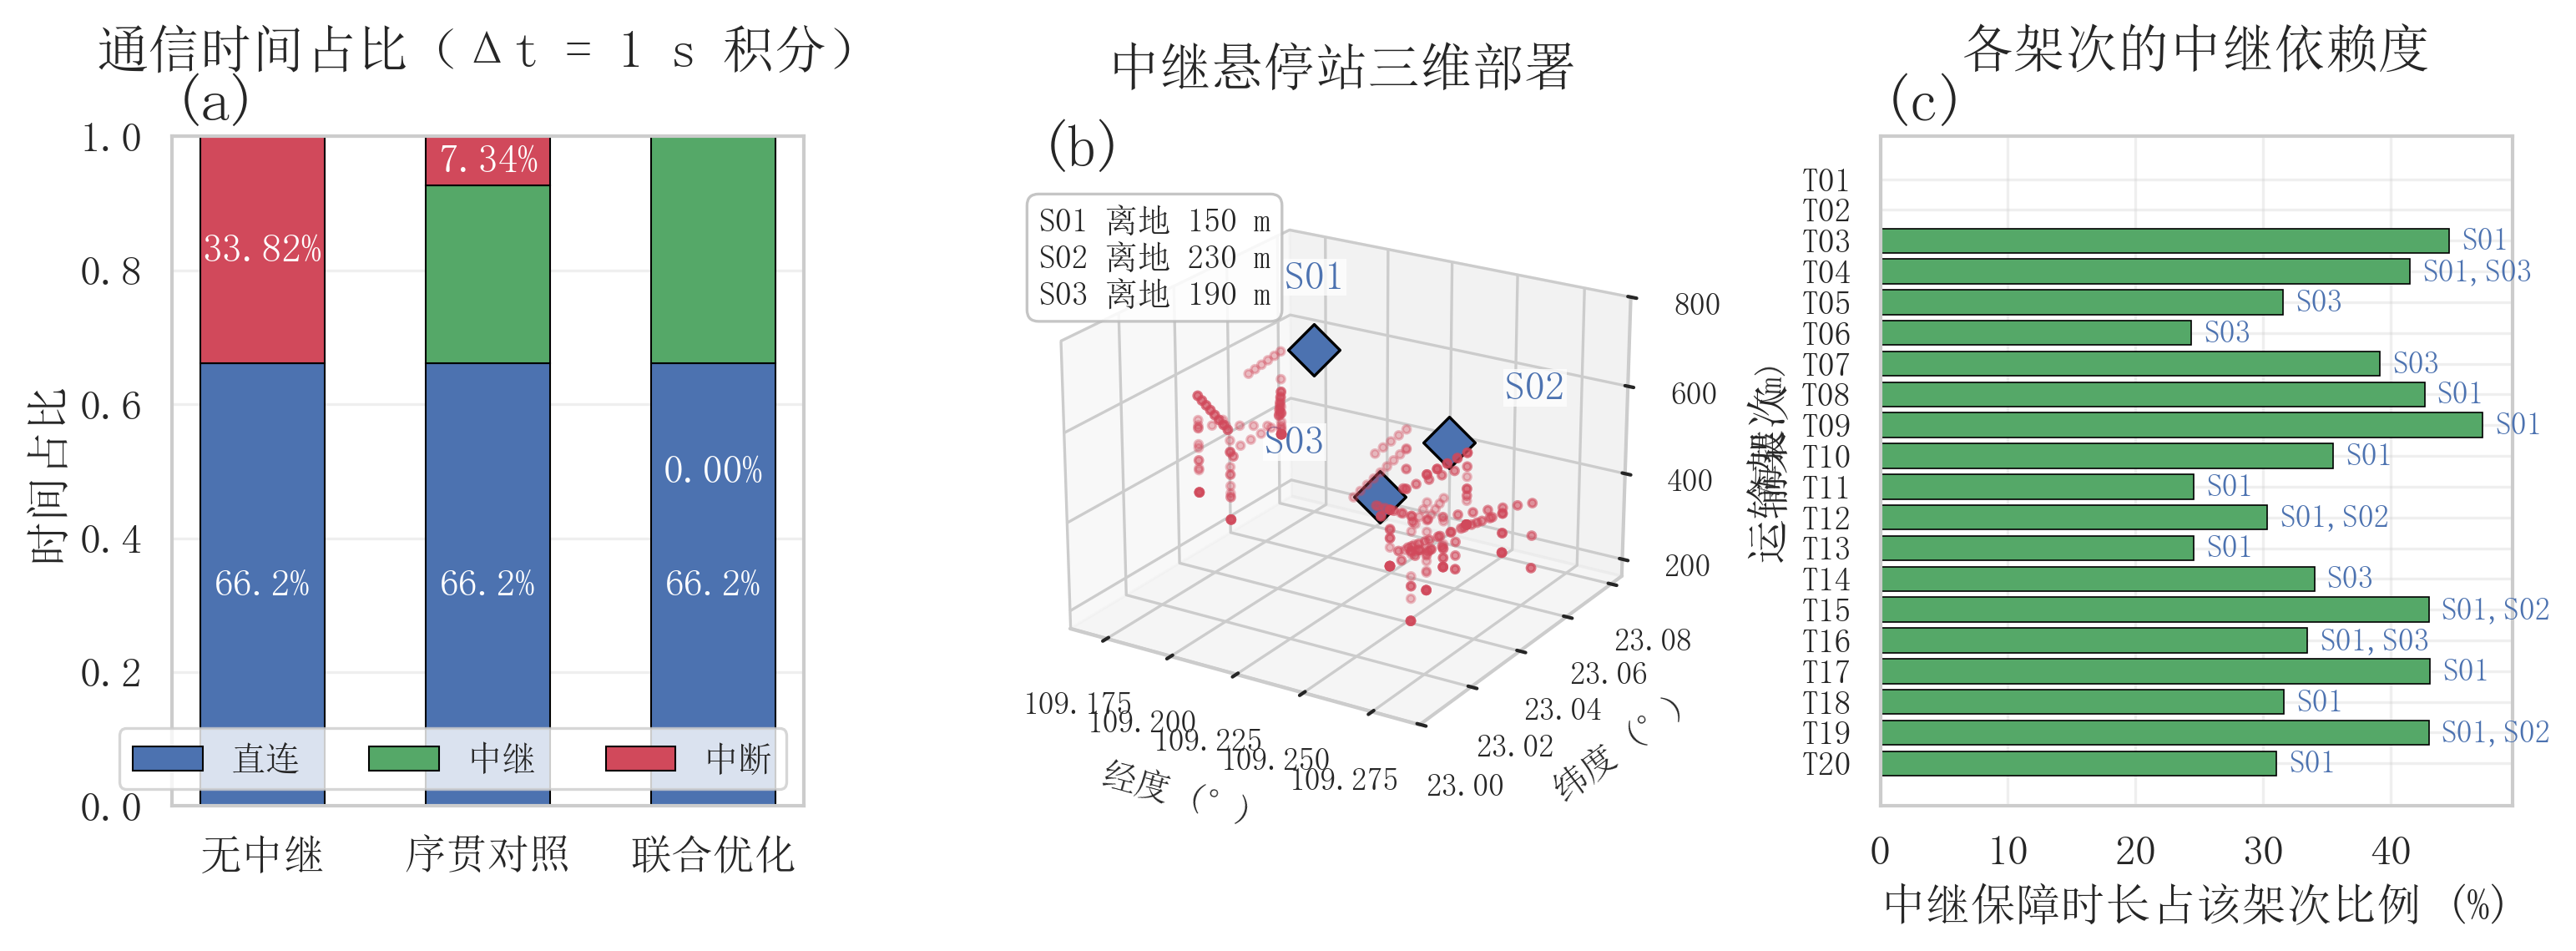
\includegraphics[width=0.95\textwidth]{figures/fig_q3_analysis.png}
	\caption{悬停站三维位置与链路裕量分布}
	\label{fig:q3-analysis}
\end{figure}

\textbf{一条未采用的并列路径（如实记录）。}本节另实现了一条「运输重排 $\leftrightarrow$ 中继归属」的固定点迭代错峰路径（\texttt{code/q3\_v2.py}），两条路径都跑完再按同一字典序择优，旧路径原地保留。实测该路径在 12 轮上限内\textbf{未收敛}：累计释放量逐轮单调增长（第 1 轮 $0$\,s $\to$ 第 12 轮 $33\,388$\,s），每轮都在把运输架次继续往后推而不进入不动点，其末端解的缺口仍有 $1694$\,s（对应 4 个失效区间无人保障），累计推迟达 $43\,342$\,s、加权迟到 $282\,463$、联合完工 $13\,108$\,s、中继能耗 $5.409$\,kWh，在字典序的每一层上都劣于现有方案。故\textbf{该路径本次未被采用}，择优判据与逐轮记录都留在运行日志中，未静默丢弃。本文据此指出：在这类「释放时刻随排班自增」的耦合问题上，固定点迭代并不自动收敛，把未收敛的迭代结果当作解使用会得到一个表面上「零弃飞」、实则留下大段盲区的方案。

\subsection{零中断的代价}
\label{sec:q3-cost}

通信连续性归零不是免费的，本文如实报告其代价。第一，\textbf{联合完工时刻由问题二的 $6506.1$\,s 推迟到 $9749.5$\,s，增加 $3243.4$\,s（$+49.9\%$）}；其中运输侧的完工由 $6506.1$\,s 推迟到 $9594.4$\,s（$+47.5\%$），其余 $155.1$\,s 是中继最晚返航造成的。第二，共有 \textbf{11 个运输架次被推迟，累计推迟 $17\,291.5$\,s}，推迟量最大的五个是 T17（$4714.5$\,s）、T23（$3097.3$\,s）、T14（$2918.3$\,s）、T04（$1718.2$\,s）、T18（$1598.4$\,s）。第三，交付侧出现 \textbf{1 个迟到货箱}（S004-WAT-03，由 T17 承运，比期望送达时刻晚 $1470.7$\,s，加权迟到合计 $14\,707.0$ 权重$\cdot$s）；该箱属饮用水、题面未给硬时限，故\textbf{货箱硬时限零违约仍然成立}，但全方案的最小硬时限余量已只剩 \textbf{$5.35$\,s}（S002-WAT-01）。第四，中继侧额外消耗 $4.493$\,kWh 与 6 组能源组件周转。

必须说明这四项代价与第 \ref{sec:q2-gate} 节的门禁之间的因果：门禁在第三问字典序里把\textbf{缺口秒数排在累计推迟量之前}，因此它选择了「用推迟换零中断」。这一排序不是任意设定的——题面把连续通信列为\textbf{约束}、把送达时刻列为\textbf{优化目标}（且饮用水只有期望时刻、没有硬时限），故先保证约束、再优化目标符合题目给出的层次。但代价是真实的：若把加权迟到置于缺口之前，原序方案（缺口 $0.6688\%$、加权迟到 $0$、累计推迟 $13\,481$\,s、中继 6 架次、$4.0457$\,kWh）会在该指标上更优，而它\textbf{在题面约束下不可行}。本文不给「两全」的假象，只报告这一取舍。

\subsection{口径说明}

本节的三组占比一律采用\textbf{时间积分口径}：以 $\Delta t=1$\,s 离散化，每点权重取 $w_i=(t_{i+1}-t_{i-1})/2$，再按状态累加，因此占比是时间占比而非采样点个数占比。这一改动是必要的：轨迹在爬升、巡航、悬停交接各段的采样密度并不相同，按点数统计会系统性偏向采样更密的阶段。此外，判定中继覆盖时须同时满足「该悬停站此刻确实能连通这架运输机」与「该中继架次此刻已完成建链且尚未结束服务」，而不能只检查时刻是否落在某个在役中继的时间窗内——后者会把「站在服务、但几何上够不着」的时段误记为已覆盖，从而虚高中继覆盖率。本文的早期版本正是采用了后一种粗口径，故其报出的覆盖率偏高、中断率偏低，最终结论以本节的逐点判定为准。

\textbf{运输侧的飞行高度不在决策空间内。}表~\ref{tab:relay-gap} 中直连占比在三组口径下恒为 $71.67\%$，除第 \ref{sec:link-model} 节已经指出的「直连可用性只取决于轨迹几何」之外，还有一个更基本的原因：运输侧的飞行高度是题面附录 2 的规定值，而非可优化的量。附录 2 规定「计划巡航海拔取该航段所经过 DEM 像元的最高地面高程以上 50 米」，且「O01 作业高度取其地面海拔，服务区作业高度取其地面海拔以上 30 米」；问题三点名的决策对象是「货箱组批与访问顺序、运输无人机及共享电池安排、各架次开始时刻，以及\textbf{中继无人机}的悬停位置、飞行海拔、服务时段和能源组件分配」——运输机的高度不在其中，只有中继机的飞行海拔是待定项，且其自由度被「悬停离地高度不超过附件规定上限」所界。这一设定并非疏漏：巡航海拔已按沿线最高地面高程留出 $50$\,m 净空，无人机相对其所在位置的地面恒有余量，但调度中心的天线高度有限，两端点之间的视线仍可能被中途地形切断——此时题面给出的补救手段是中继，而不是让运输机改飞一条附录 2 未作规定的轨迹。提交要求又明确「公共物理规则、单位、对象编号和计算口径应保持一致」，故抬高运输巡航高度还会使问题三与问题一、二的能耗与时间口径脱钩，本节不予采用。

需要说明的是，地形对链路的高度敏感性并未因此被搁置，它恰好由中继侧接管：表~\ref{tab:q3-stations} 五站的离地高度都是决策变量，其中两站取到 $300$\,m 上限，这是本题允许抬高飞行海拔的唯一一侧。
         % 七、问题三
\section{问题四：救援任务分区与资源配置}

题面要求把 15 个服务区划分为 2 组或 3 组并行开展救援，并明确「各任务组\textbf{分别核算}独立执行所需资源，\textbf{任务执行期间各类资源不得跨组调配}」。这一条把问题从「如何分组更均衡」变成了「分组后还能不能落地」：资源不可跨组复用，意味着每组都必须自备完整的运输与通信保障能力。本节据此建立分区模型、给出完全枚举结果，并如实核算缺口。

\subsection{原子任务单元与完全枚举}

\textbf{不可再拆的原子单元。}分区不能任意切割服务区：若两个服务区在问题三的推荐方案中被同一运输架次访问，则它们在同一组内才能共享那一架次，拆开会使架次方案失效。故先以「被同一架次服务」为边构建服务区之间的必连图，取连通分量为\textbf{原子任务单元}。按问题三联合方案计算，24 个运输架次把 15 个服务区归并为 \textbf{12 个原子单元}（表~\ref{tab:q4-units}），其中 2 个单元（U01、U08）含多个服务区。

\begin{table}[htbp]
	\caption{原子任务单元及其工作量}
	\label{tab:q4-units}
	\centering
	\small
	\begin{tabular}{clcc}
		\toprule
		编号 & 服务区列表 & 运输架次数 & 工作量（h） \\
		\midrule
		U01 & S001, S010, S014 & 5 & 2.6113 \\
		U02 & S002 & 2 & 1.1460 \\
		U03 & S003 & 2 & 1.3072 \\
		U04 & S004 & 3 & 1.6760 \\
		U05 & S005 & 1 & 0.5221 \\
		U06 & S006 & 3 & 1.0677 \\
		U07 & S007 & 3 & 1.4109 \\
		U08 & S008, S011 & 1 & 0.7475 \\
		U09 & S009 & 1 & 0.4335 \\
		U10 & S012 & 1 & 0.5401 \\
		U11 & S013 & 1 & 0.4171 \\
		U12 & S015 & 1 & 0.5083 \\
		\bottomrule
	\end{tabular}
\end{table}

\textbf{完全枚举而非启发式。}12 个单元的分区规模由第二类 Stirling 数给出：$K=2$ 时 $S(12,2)=2047$ 种，$K=3$ 时 $S(12,3)=86\,526$ 种。这一规模仍然完全可以穷举，故本文用受限增长串直接枚举全部非空无序划分（不重不漏，实测枚举数 $2047$ 与 $86\,526$ 均与理论值一致），\textbf{枚举结果即全局最优}，无需迭代搜索。这一条在本题不是可有可无的：下一节将看到，可行分区在全部枚举中一个都不存在，而那正是\textbf{只能靠枚举才能下的结论}——任何单个分区上的缺口核算都无法排除「换个分法就够了」。

\textbf{工作量的口径。}单元的工作量取该单元所含运输架次的飞行器时之和（表~\ref{tab:q4-units}）；而组的工作量还要计入分配给该组的中继飞行器时——分组的意义正在于每组自备完整的运输与通信能力，只算运输侧会低估主力组与小组的差距。故记
\begin{equation}
	W_g=\sum_{p\in \mathcal{P}_g} T_p \;+\; \sum_{k\in \mathcal{K}_g} T^{R}_{k},
	\label{eq:q4-workload}
\end{equation}
其中 $T_p$ 为运输架次 $p$ 的作业时长、$T^{R}_{k}$ 为中继架次 $k$ 从起飞到返航的时长；组间均衡度取变异系数 $CV_W=\sigma(W_1,\dots,W_K)/\bar W$。

为排除单一实现的偏差，本文另用\textbf{组列集合划分整数规划}走第二条路径复核：对每个非空单元子集预生成「组列」，再求恰好 $K$ 组的集合划分最优值。两条路径给出相同的最优资源规模 $R$（$K=2$ 为 31、$K=3$ 为 34），沿用问题一的双路径验证范式。

\subsection{资源需求核算}

对每个任务组，各类资源需求按其\textbf{独立执行时的峰值并发量}核算，而非简单取架次数：

\begin{itemize}
	\item 运输无人机：该组架次占用区间 $[\text{开始},\text{结束}]$ 的重叠峰值，按机型分别统计；
	\item 共享电池：占用区间延伸到充电完成，即 $[\text{开始},\text{结束}+T^{\text{charge}}]$ 的重叠峰值；
	\item 中继无人机：该组所需中继任务的占用区间 $[\text{起飞},\text{返航}+T^{\text{turnover}}]$（周转时间 $300$\,s）的重叠峰值，与 7.4 节中继架次调度的占用口径一致；
	\item 中继能源组件：占用区间取 $[\text{起飞},\text{返航}+\text{充电完成}]$ 的重叠峰值，充电时长按返航 SOC 反算。
\end{itemize}

需要说明的是，若某个中继架次同时服务了属于两个不同任务组的失效区间，则两组\textbf{各配一架}并如实重复计入。这正是分区带来的真实代价，不得为了数字好看而悄悄合并——资源既然不得跨组调配，同一架中继机就不可能同时属于两组。

\begin{table}[htbp]
	\caption{两类分区方案的资源需求}
	\label{tab:q4-partition}
	\centering
	\small
	\begin{tabular}{cccccccc}
		\toprule
		$K$ & 组号 & 服务区数 & A机/B机/C机 & A电/B电/C电 & 中继机 & 中继组件 & 工作量（h） \\
		\midrule
		2 & 组1 & 12 & 4/1/2 & 6/2/4 & 2 & 4 & 15.5822 \\
		2 & 组2 & 3  & 0/1/0 & 0/2/0 & 1 & 2 & 3.4651 \\
		\addlinespace
		3 & 组1 & 10 & 4/1/2 & 6/2/3 & 2 & 4 & 14.8347 \\
		3 & 组2 & 2  & 0/0/1 & 0/0/1 & 1 & 1 & 1.3446 \\
		3 & 组3 & 3  & 0/1/0 & 0/2/0 & 1 & 2 & 3.4651 \\
		\bottomrule
	\end{tabular}
\end{table}

\subsection{分区方案比较与资源缺口}

从资源规模、均衡度与缺口三方面比较两类方案，汇总于表~\ref{tab:q4-compare}。

\begin{table}[htbp]
	\caption{两类分区方案的资源规模、均衡度与缺口}
	\label{tab:q4-compare}
	\centering
	\small
	\begin{tabular}{lcccc}
		\toprule
		$K$ & 枚举分区数 & 最优资源规模 $R$ & 工作量均衡 $CV_W$ & 库存可行分区数 \\
		\midrule
		2 & 2047 & \textbf{31} & \textbf{0.6362} & \textbf{0} \\
		3 & 86\,526 & \textbf{34} & \textbf{0.9045} & \textbf{0} \\
		\bottomrule
	\end{tabular}
\end{table}

\textbf{资源规模与均衡度。}$K=2$ 的最优资源规模 $R=31$、$K=3$ 为 $R=34$，即多分一组要多配 3 件资源。均衡度上，$K=3$ 的 $CV_W=0.9045$ 反而\textbf{大于} $K=2$ 的 $0.6362$——这与「组数越多越均衡」的直觉相反，原因是原子单元的工作量本身极不均匀：最重的 U01 一个单元就占 2.6113\,h，约为最轻的 U11（0.4171\,h）的 6.3 倍，12 个单元合计仅 12.39\,h。在最小化资源规模的目标下，最优解会把大头集中在一组、让小单元各自成组，于是 $K=3$ 把只含一个架次的 U08（S008、S011，0.7475\,h）单独拆成一整组，该组工作量 1.34\,h，均衡度反倒恶化（表~\ref{tab:q4-partition}中 14.83\,h 对 1.34\,h 与 3.47\,h）。这说明\textbf{均衡与省资源在本问题上是一对真实的冲突}，需要按目标选择，而不是默认多分组更好。

\textbf{资源缺口（逐类）。}以库存为基准逐类核算需求与缺口，结果如表~\ref{tab:q4-gap}所示。表中「需求」是\textbf{推荐分区}的需求，按总量口径核算——即全队共用同一份库存时，$K$ 个组各自的峰值需求叠加后有没有超出库存。这是「这套分区能不能落地」的正确判据：资源既然不得跨组调配，每个组占住的机器在它自己的作业期间就归它专用，总量必须逐组相加。要判断某一类缺口是不是分区的必然后果，还要看该类在全部 2047 与 $86\,526$ 个分区上的最小需求（表~\ref{tab:q4-min}）。

\begin{table}[htbp]
	\caption{逐类资源需求、库存与缺口}
	\label{tab:q4-gap}
	\centering
	\small
	\begin{tabular}{lcccccc}
		\toprule
		\multirow{2}{*}{资源类别} & \multicolumn{3}{c}{$K=2$} & \multicolumn{3}{c}{$K=3$} \\
		\cmidrule(lr){2-4}\cmidrule(lr){5-7}
		 & 需求 & 库存 & 缺口 & 需求 & 库存 & 缺口 \\
		\midrule
		A 型运输无人机 & 4 & 4 & 0 & 4 & 4 & 0 \\
		B 型运输无人机 & 2 & 2 & 0 & 2 & 2 & 0 \\
		C 型运输无人机 & 2 & 2 & 0 & 3 & 2 & \textbf{1} \\
		A 型共享电池   & 6 & 6 & 0 & 6 & 6 & 0 \\
		B 型共享电池   & 4 & 4 & 0 & 4 & 4 & 0 \\
		C 型共享电池   & 4 & 4 & 0 & 4 & 4 & 0 \\
		中继无人机     & 3 & 2 & \textbf{1} & 4 & 2 & \textbf{2} \\
		中继能源组件   & 6 & 6 & 0 & 7 & 6 & \textbf{1} \\
		\bottomrule
	\end{tabular}
\end{table}

\begin{table}[htbp]
	\caption{全部分区中的最小需求：区分推荐分区的缺口与结构性缺口}
	\label{tab:q4-min}
	\centering
	\small
	\begin{tabular}{lcccccc}
		\toprule
		\multirow{2}{*}{资源类别} & \multicolumn{3}{c}{$K=2$（2047 个分区）} & \multicolumn{3}{c}{$K=3$（$86\,526$ 个分区）} \\
		\cmidrule(lr){2-4}\cmidrule(lr){5-7}
		 & 最小需求 & 库存 & 最小缺口 & 最小需求 & 库存 & 最小缺口 \\
		\midrule
		A 型运输无人机 & 4 & 4 & 0 & 4 & 4 & 0 \\
		B 型运输无人机 & 2 & 2 & 0 & 2 & 2 & 0 \\
		C 型运输无人机 & 2 & 2 & 0 & 2 & 2 & 0 \\
		A 型共享电池   & 6 & 6 & 0 & 6 & 6 & 0 \\
		B 型共享电池   & 4 & 4 & 0 & 4 & 4 & 0 \\
		C 型共享电池   & 4 & 4 & 0 & 4 & 4 & 0 \\
		中继无人机     & 2 & 2 & 0 & 3 & 2 & \textbf{1} \\
		中继能源组件   & 4 & 6 & 0 & 4 & 6 & 0 \\
		\bottomrule
	\end{tabular}
\end{table}

\textbf{核心结论：按题目「资源不得跨组调配」的规则，$K=2$ 与 $K=3$ 在现有库存下均不可行。}2047 个与 $86\,526$ 个分区中，满足总量口径资源约束的分区数为 \textbf{0}。但两者不可行的成因\textbf{并不相同}，需要分开说清楚——把两种成因混为一谈会得出过强的结论：

\begin{enumerate}
	\item \textbf{$K=3$ 的中继无人机是\textbf{结构性}短缺。}题目要求资源不得跨组调配，则每个非空任务组都必须自备通信保障能力；本算例的 19 个失效区间遍布各组，故\textbf{每个非空组至少要占 1 架中继无人机}。$K=3$ 有 3 个非空组，全部分区中继无人机总需求的最小值就是 $3$，而库存只有 $2$ 架（表~\ref{tab:q4-min}「中继无人机」行最小缺口 $1$）。这一架缺口\textbf{与怎么分组无关}：只要分成 3 个都含失效区的组，就必然短缺一架，枚举 86\,526 个分区也躲不掉。
	\item \textbf{其余各类在 $K=2$、$K=3$ 下都不是结构性短缺。}把每一类资源单独拿出来看它在全部分区上的最小需求（表~\ref{tab:q4-min}），除 $K=3$ 的中继无人机外，其余各类（含 $K=2$ 的中继无人机）的\textbf{最小缺口均为 0}：A 型运输无人机最小只需 4 架、B 型与 C 型运输无人机各 2 架、三类共享电池的最小需求分别为 6/4/4 组、中继能源组件 4 个——每一项都\textbf{不超过库存}。也就是说，单独针对这些类别中的任何一类，都存在一个不超库存的分区。$K=2$ 时中继无人机的最小需求恰为 2 架、正好等于库存，正是上述「每组一架」机制的临界情形。
	\item \textbf{第二重来源：联合约束。}对 $K=2$，不可行性无法归因于任何单类短缺（第 2 条），故只能来自联合约束：由第 2 条与「可行分区数为 0」可直接推出，\textbf{不存在任何一个分区能同时取到八类资源各自的最小值}——若存在，该分区各类需求就都等于对应最小值、都不超库存，它本身就会是一个可行分区，与枚举结果矛盾。于是「逐类看处处有余量」与「整体看无一处可行」并存。$K=3$ 则是两种成因叠加：中继无人机的结构性缺口已足以判定不可行，联合约束在此之外仍然存在。
	\item \textbf{推荐分区的缺口是「省资源＋求均衡」这一目标的代价，但其中一部分消不掉。}按 $R$ 最小、$CV_W$ 次小选出的推荐分区（表~\ref{tab:q4-partition}）需要：$K=2$ 缺中继无人机 1 架，合计 1 件；$K=3$ 缺 C 型运输无人机 1 架、中继无人机 2 架、中继能源组件 1 件，合计 4 件。$K=2$ 的那一件与 $K=3$ 的非中继部分\textbf{可以分别}靠换一个分区消去（表~\ref{tab:q4-min} 中相应类别都有取到库存水平的分区），但\textbf{不能同时}消去（第 3 条）；而 $K=3$ 中继无人机缺口中的那 1 架是结构性的（第 1 条），\textbf{换任何分区都消不掉}。
\end{enumerate}

\textbf{与「分区放大需求」这一直觉的关系。}分组推高需求的机制是各组峰值叠加：某类资源在单个组内的峰值也许远小于库存，但 $K$ 组同时作业时占用之和仍可能超过那一份共享库存。本算例的枚举表明，这个效应在 $K=2$ 时确实\textbf{不足以}构成任何单类资源的结构性缺口，但在 $K=3$ 时对中继无人机\textbf{恰好越过了临界点}——因为中继无人机库存只有 2 架，而「每组一架」的下界随组数增长，$K=3$ 时 $3>2$。把这一条与联合约束混为一谈，会得出「$K=3$ 也只是联合约束问题」的过强结论，本文不作此表述。

\textbf{落地建议。}按题意「资源不得跨组调配」的硬判据，两类分区在现有库存下都不可行，且完全枚举证明这\textbf{不是换一种分法就能回避的}（可行分区数为 0）。因此：

\begin{itemize}
	\item 若必须分区，就需要扩充机队，扩充清单取决于所选分组数与分区。按推荐分区计：$K=2$ 需补中继无人机 1 架；$K=3$ 需补 C 型运输无人机 1 架、中继无人机 2 架、中继能源组件 1 件。其中\textbf{$K=3$ 的中继无人机缺口有 1 架是结构性的}，无论改选哪个分区都必须补；其余各项若愿意牺牲资源规模 $R$ 与均衡度 $CV_W$，可改选缺口更小的分区，但不可能降到 0。
	\item 若不扩充机队，更现实的结论是\textbf{不分区}：以问题三的单组联合方案整体执行，其资源需求不超过现有库存（8 架运输无人机与 14 组共享电池全部投入周转，见 6.4 节），而分区虽然在调度视角上便于并行，却在本题「资源不得跨组调配」的规则下不可行。
\end{itemize}

图~\ref{fig:q4-resource}以雷达图与缺口柱状图并列展示两类方案在八类资源上的需求分布与缺口构成；图~\ref{fig:q4-partition}则给出原子单元之间的必连关系、各单元工作量的空间分布以及两类分区下的资源规模分布。

\begin{figure}[htbp]
	\centering
	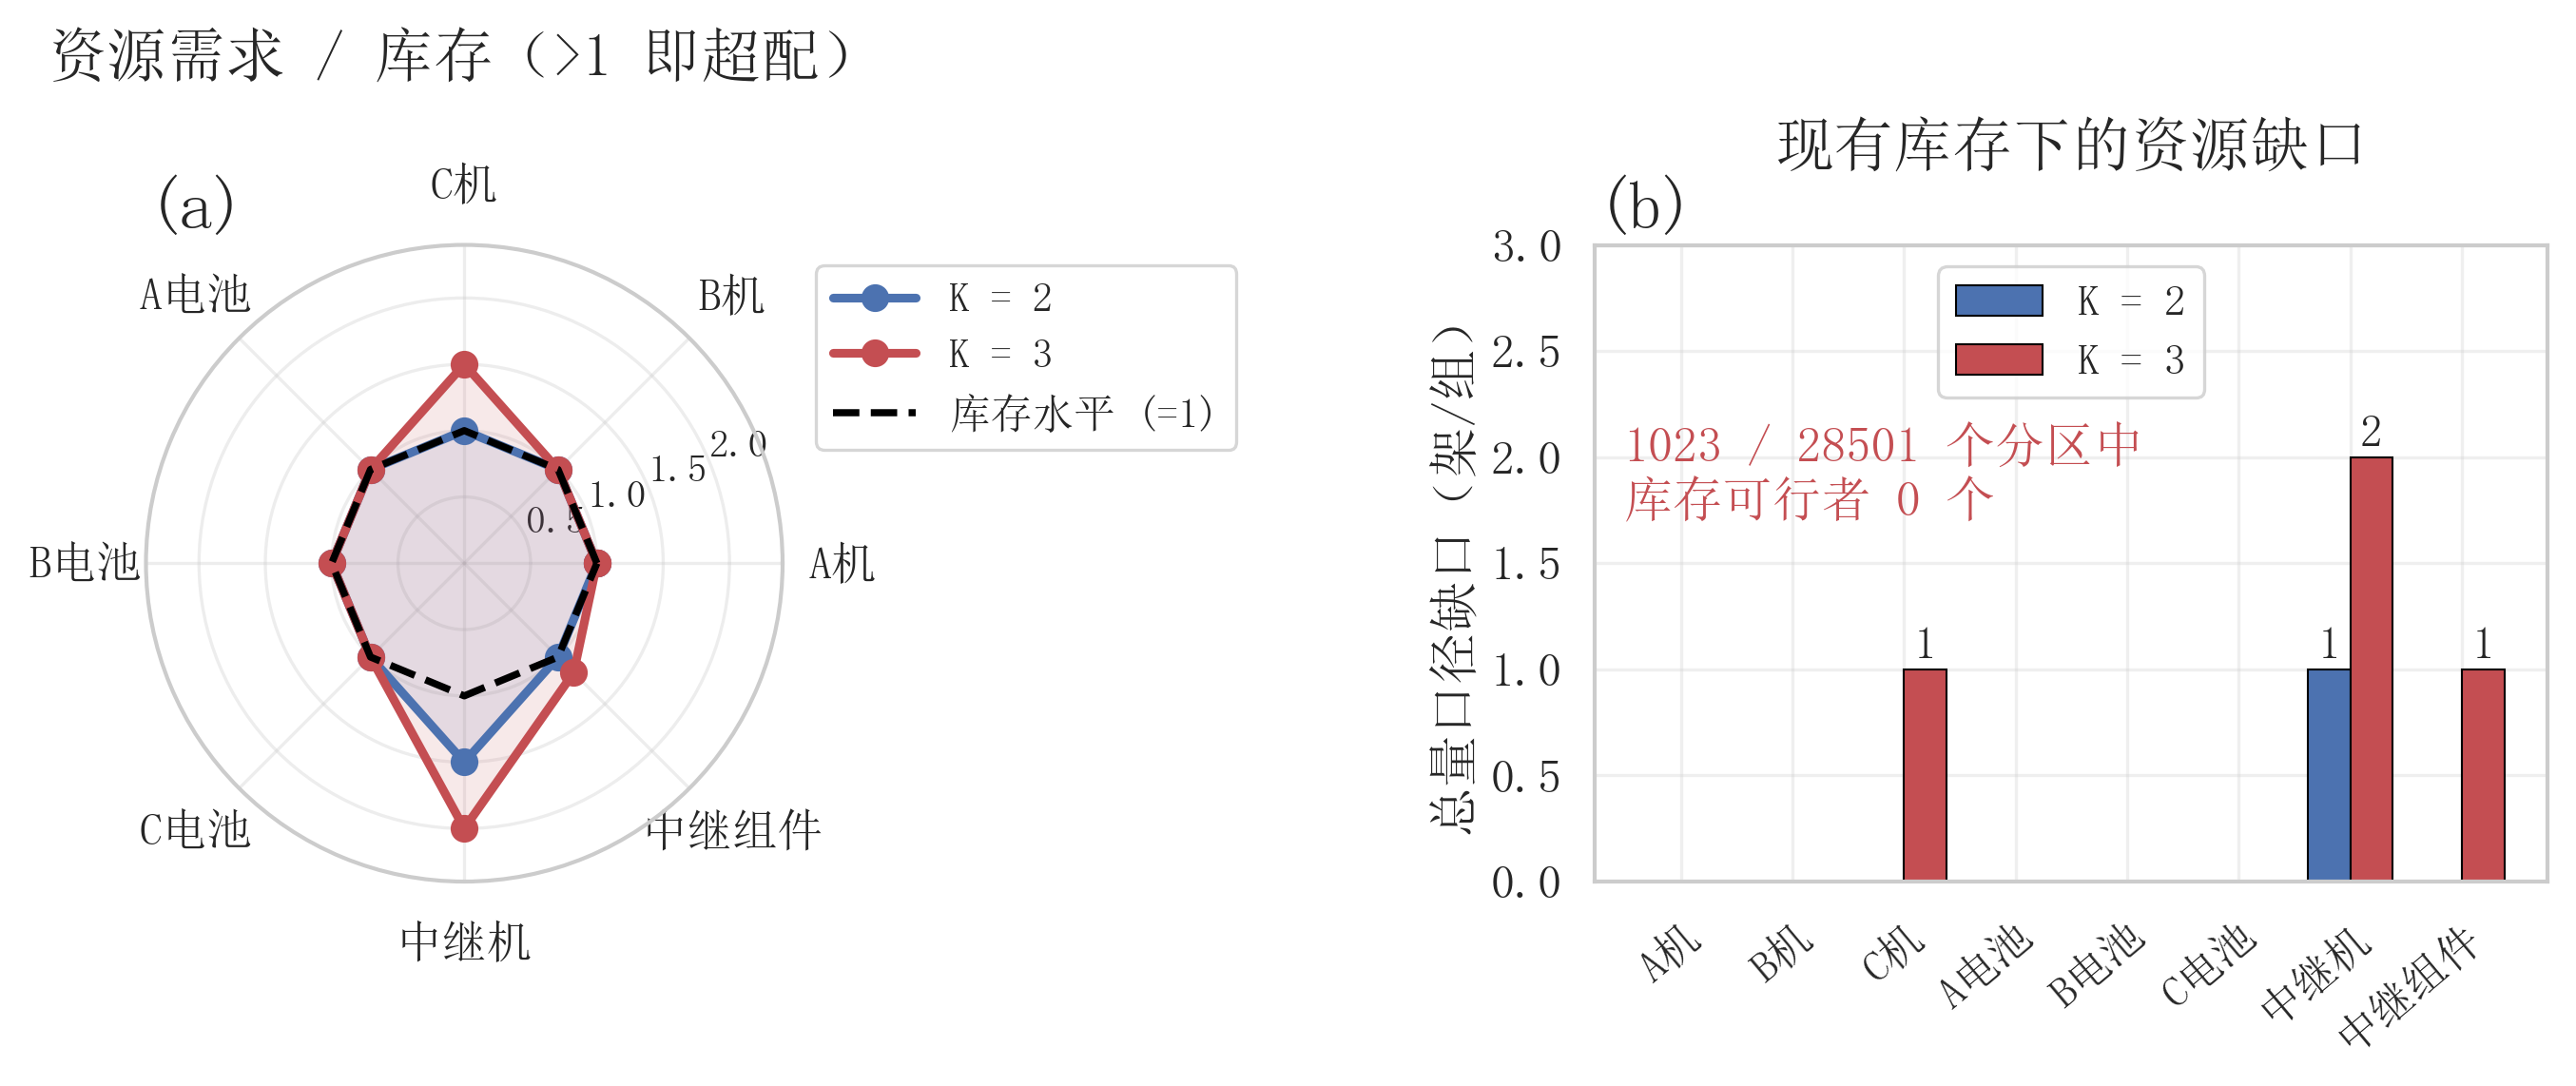
\includegraphics[width=0.95\textwidth]{figures/fig_q4_resource.png}
	\caption{两类分区的资源需求与缺口}
	\label{fig:q4-resource}
\end{figure}

\begin{figure}[htbp]
	\centering
	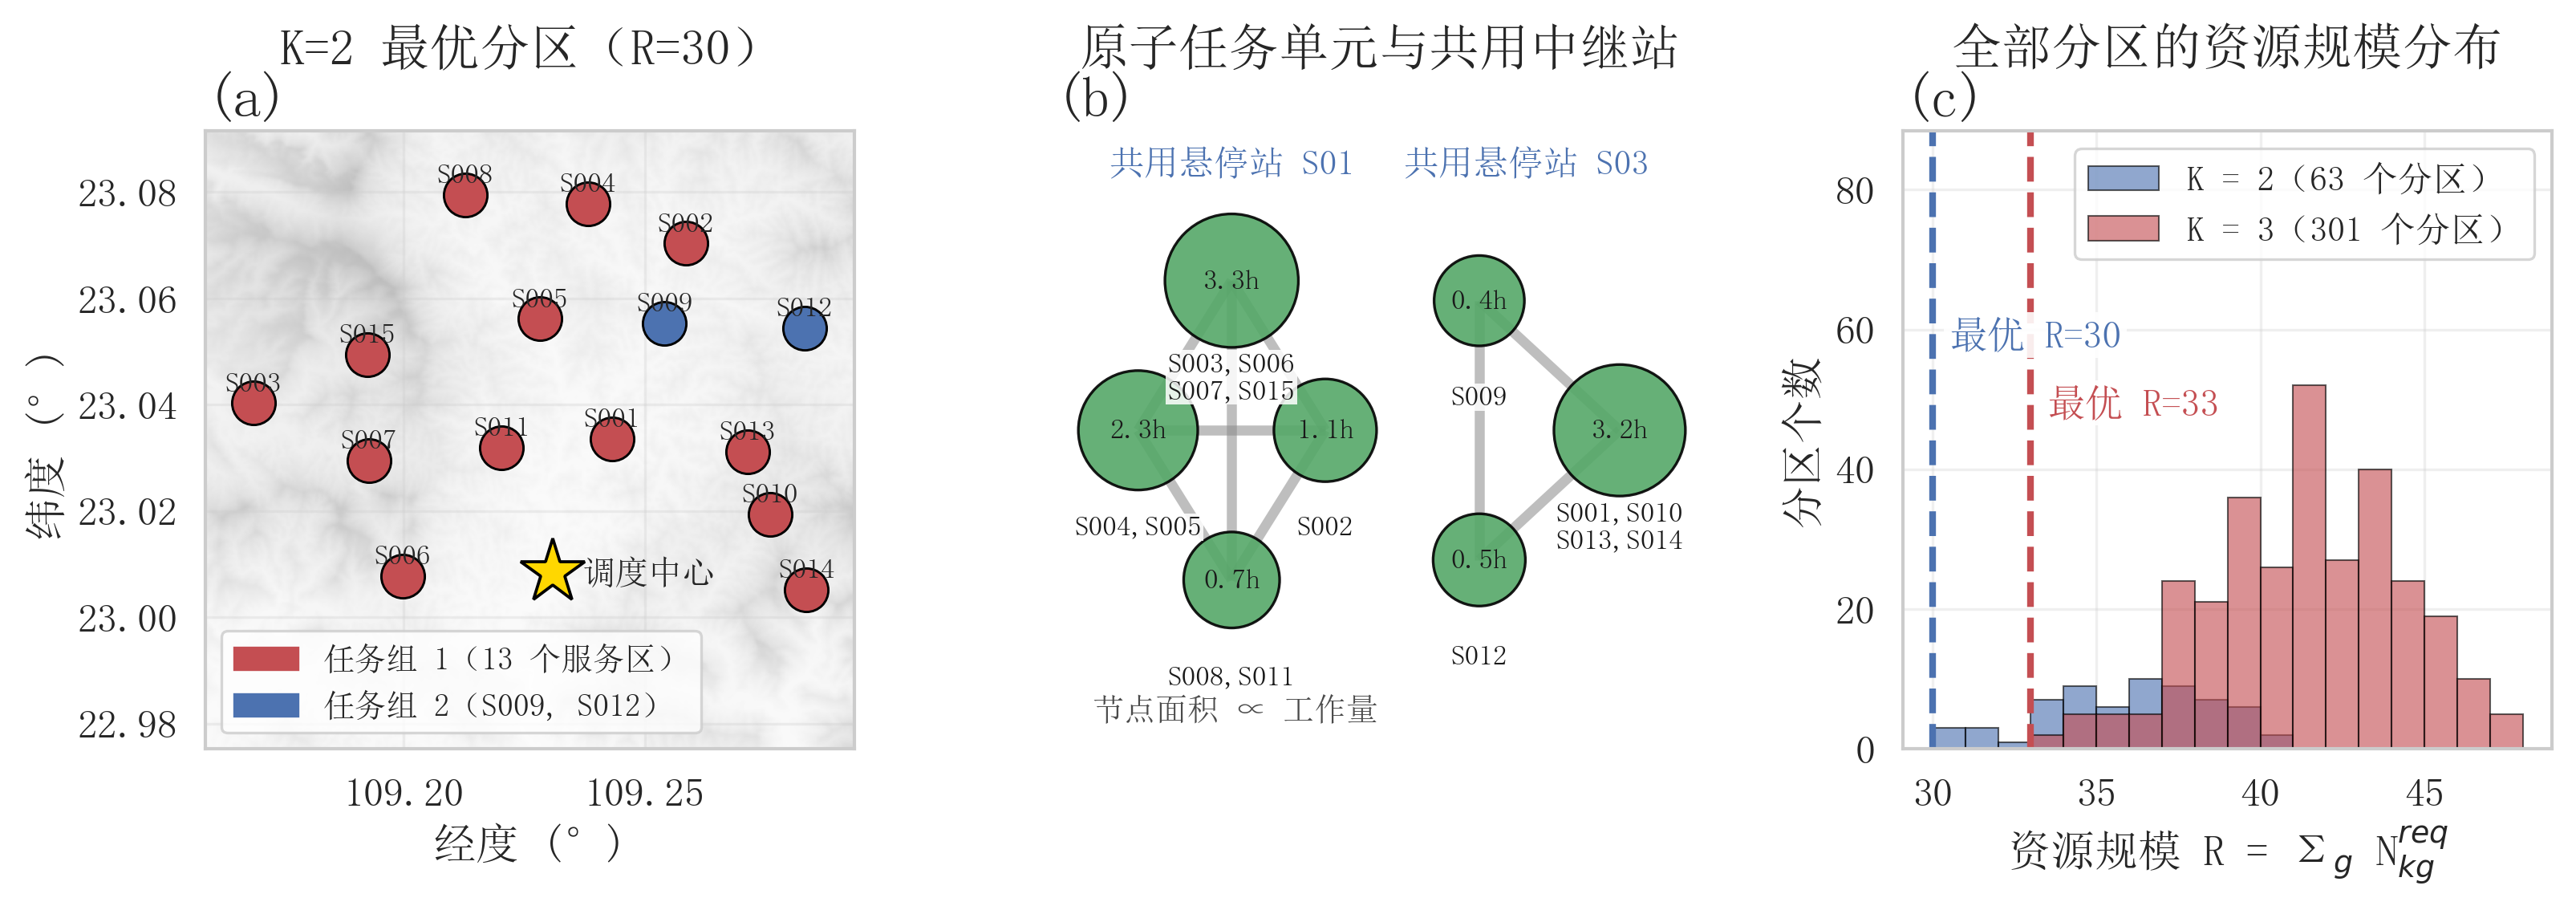
\includegraphics[width=0.95\textwidth]{figures/fig_q4_partition.png}
	\caption{原子任务单元与两类分区资源分布}
	\label{fig:q4-partition}
\end{figure}
         % 八、问题四
\section{模型检验与分析}

为验证本文模型的有效性与稳健性，从可行性检验、敏感性分析与结果交叉验证三方面进行。需要强调的是，可行性检验若仅由求解程序自报，无法排除程序内部状态出错的可能。为此本文另写独立复核脚本 \texttt{code/verify.py}，\textbf{只读四问的结果表}（不调用求解器的任何中间变量）重新计算四问的硬约束，结果分别见表~\ref{tab:q1check}--\ref{tab:q4check}（其中表~\ref{tab:q1ilp}、表~\ref{tab:q3metrics}、表~\ref{tab:q3chain}是本轮为问题一的第二路径与问题三的交付侧、资源链新增的三项复核）。该脚本同时复现 9.4 节的 DEM 离散化误差，代码清单见附录~\ref{tab:code-list}。这里须说明复核的边界：脚本与求解器仍共享公共物理模块 \texttt{core.py}（地形净空、能耗、充电、链路），因此它排除的是\textbf{求解程序内部状态与结果表之间的串号、漏检与自我印证}，并不能排除公共物理模型本身的口径错误——后者只能靠 9.4 节的口径对照与原始数据判读，不能被「两份程序算得一致」所替代。

\subsection{可行性检验}
\label{sec:q3-check}

\begin{center}
\begin{minipage}{\textwidth}
	\captionof{table}{问题一推荐组批方案的独立复核}
	\label{tab:q1check}
	\centering
	\begin{tabularx}{0.98\textwidth}{lXcc}
		\toprule
		复核项 & 判据 & 实测 & 越限 \\
		\midrule
		覆盖完整性 & 80 个货箱各被引用恰一次 & 重复 0、漏交 0、孤儿引用 0 & 0 \\
		载重与容积 & 每架次质量、体积均不超机型上限 & 越限 0 处 & 0 \\
		能量安全余量 & 架次能耗 $\le (1-\rho_g)E_g^{\mathrm{use}}$ & 越限 0 处 & 0 \\
		独立重算偏差 & 逐架次重算能耗与时间并与结果表比对 & 能耗 $4.97\times10^{-7}$\,kWh、时间 $4.97\times10^{-4}$\,s & 0 \\
		机型架次自洽 & 明细表与汇总表的架次分布一致 & B 型 7、C 型 11，两表一致 & 0 \\
		\bottomrule
	\end{tabularx}
\end{minipage}
\end{center}

问题一的复核共 18 个架次。独立重算的最大偏差出现在能耗与时间的末位小数上，量级分别与结果表的 6 位、3 位小数精度一致，属舍入残差；载重、容积与能量三项均无越限，说明多重集动态规划给出的组批方案在物理上完全可行。

除上述逐架次重算外，问题一还须回答一个方法论问题：5.2 节用「多重集动态规划」与「集合划分整数规划」两条路径求解，两条路径是否真的给出同一答案？表~\ref{tab:q1ilp}把这一核对单列出来，逐区比较两法的\textbf{最少架次数}，并在该架次数下比较总能耗。

\begin{center}
\begin{minipage}{\textwidth}
	\captionof{table}{问题一集合划分整数规划的交叉复核}
	\label{tab:q1ilp}
	\centering
	\begin{tabularx}{0.98\textwidth}{lXcc}
		\toprule
		复核项 & 判据 & 实测 & 不符 \\
		\midrule
		区域数 & 逐区核对（共 15 个服务区） & 15 个 & 0 \\
		两法一致性 & 最少架次数相等，且该架次数下能耗差 $<10^{-6}$\,kWh & 一致 14、不一致 0 & 0 \\
		未复核项 & 求解器未在时限内证明最优者如实列出、不冒充 & 1 个（S001，阶段 2 报 \texttt{Time limit}） & --- \\
		\bottomrule
	\end{tabularx}
\end{minipage}
\end{center}

表~\ref{tab:q1ilp}第 3 项是这一节最该讲清楚的一格：15 个服务区中有 1 个（S001）整数规划未能在时限内\textbf{证明}最优，故它既不算「一致」也不算「不一致」，而是明确记为\textbf{未复核}。若把这一格悄悄并入「一致」，就变成用 14 个区的结论去冒充 15 个区——本文不这样做。即便如此，两法在 14 个可复核区域上最少架次数与能耗全部相同，说明 5.2 节两条路径的互证是成立的；S001 的组批结果仍由逐架次物理复算（表~\ref{tab:q1check}）兜底，只是缺少「最优性」这一层互证。

\begin{center}
\begin{minipage}{\textwidth}
	\captionof{table}{问题二推荐方案的硬约束独立复核}
	\label{tab:hardcheck}
	\centering
	\begin{tabularx}{0.98\textwidth}{lXcc}
		\toprule
		复核项 & 判据 & 实测最紧值 & 越限 \\
		\midrule
		能量裕度 & 架次能耗 $\le (1-\rho_g)E_g^{\mathrm{use}}$ & 占用比最大 0.996（均值 0.671） & 0 \\
		无人机占用 & 同一实体无人机任一时段不重叠 & 重叠 0 处 & 0 \\
		电池周转 & 同一电池充电完成后方可再起飞 & 最小间隙 $-1\times10^{-4}$\,s$^{\dagger}$ & 0 \\
		物资时限 & 医疗期望与首批截止时刻 & 违约 0 箱 & 0 \\
		交付完整性 & 80 箱各交付一次且架次号有效 & 重复 0、漏交 0、孤儿引用 0 & 0 \\
		资源库存 & A/B/C 用机 $\le 4/2/2$、用电池 $\le 6/4/4$ & 用机 $4/4$、$2/2$、$2/2$；电池 $6/6$、$4/4$、$4/4$ & 0 \\
		\bottomrule
	\end{tabularx}
\end{minipage}
\end{center}

$^{\dagger}$ 周转间隙由“返回时刻＋按能耗反算的充电时长”推得，时刻列保留 3 位小数、能耗列保留 6 位小数，舍入噪声约 $5\times10^{-4}$\,s；复核容差取 $0.01$\,s，比舍入噪声高一个量级、比任何真实调度冲突小两个数量级。实测最小间隙为 $-1\times10^{-4}$\,s，\textbf{为负}，但绝对值仅为舍入噪声的 $1/5$，即它是「两列小数各自舍入后相减」产生的残差，而不是真实的周转冲突：若真存在冲突，其量级应是分钟乃至小时（充电本身以千秒计），不会落在 $10^{-4}$\,s。这里必须把话说准：这一项的支持证据是\textbf{间隙绝对值远小于舍入噪声}，而非「间隙为正」——上一版论文写「为正」是因为当时的解在末尾恰好凑出正残差，换解之后符号翻转，若沿用「为正」这一措辞就会得出相反结论，故此处按残差量级重述。可见推荐方案的 24 个架次在全部硬约束上可行，且现有库存被\textbf{完全投入}（8 架运输无人机、14 组共享电池全部参与周转）。这里须区分“事实”与“结论”：资源全部投入是该解的一个事实，\textbf{不等于}已逼近产能上界——那需要证明在同样资源下不存在完工时间更短的可行解，本文并未证明（§6.3 的精确验证只覆盖 3 个服务区的小算例，且 $K\le20$ 是外部给定的扫描档位、并非由资源上限推出）。因此本节只能说：在该档位上解已用满库存，若进一步收紧时限，是否仍存在可行解需要重新搜索才能回答。

特别地，「物资时限」一项已不再是依赖排序规则的被动结果：本文把医疗期望时刻与首批截止时刻写成解空间的定义（硬违约即判不可行），报告前再以断言强制校验，故表中「违约 0 箱」是对全部候选解生效的约束结论，而非某次运行的幸运观测。

\begin{center}
\begin{minipage}{\textwidth}
	\captionof{table}{问题三中继方案的独立复核}
	\label{tab:relaycheck}
	\centering
	\begin{tabularx}{0.98\textwidth}{lXcc}
		\toprule
		复核项 & 判据 & 实测最紧值 & 越限 \\
		\midrule
		能量裕度 & 架次能耗 $\le(1-\rho_R)E_R^{\mathrm{use}}$ & 占用比最大 0.439（可用 2.56\,kWh/架次） & 0 \\
		悬停高度 & 悬停离地 $\le$ 题给上限 & 最大 300.0\,m（上限 300\,m，取到上限） & 0 \\
		中继占用 & 同一中继无人机任一时段不重叠 & 重叠 0 处 & 0 \\
		组件周转 & 能源组件充电完成后方可再投入 & 冲突 0 处 & 0 \\
		结果表自洽 & 「中继」段须落在某架次服务窗口内 & 标注不符 0 段 & 0 \\
		\bottomrule
	\end{tabularx}
\end{minipage}
\end{center}

表~\ref{tab:relaycheck}中悬停离地高度一项不采信结果表记录的数值，而是取表内经纬度回原始 DEM 重新插值出地面高程，再与记录的海拔相减复核；能源组件的可用时刻同样由“返回时刻＋按能耗反算的充电时长”重新推得，与求解器内部状态无关。复核显示 7 个中继架次的能耗占用比最高仅 0.439，远未触顶。这只说明\textbf{当前方案的}中继能量约束未紧绑定，限制中继能力的是\textbf{时序结构}与\textbf{站址几何}：两架中继无人机的航链首尾相接（R01 三段、R02 四段），能同时出动的架次受链长约束；而 3 站取中间档、2 站顶到 300\,m 上限，说明限制选址的是\textbf{接入余量}而不是能量（7.3 节已就此说明：\texttt{refine\_station} 以最大化最小接入余量为目标，高度是被余量推上去的，不是被能耗推上去的）。这两点与 7.6 节关于推迟量成因的分析一致。需注意该观察不能外推：换悬停站、加大服务窗口或放宽并发都会改变能量占用比，届时能量完全可能先触顶；本文由此只能得出“本方案的瓶颈在时序与几何”这一条结论，不能得出“中继能量永远不会成为瓶颈”。

\begin{center}
\begin{minipage}{\textwidth}
	\captionof{table}{通信连续性的独立复核（$\Delta t=1$\,s 逐时刻重判）}
	\label{tab:commcheck}
	\centering
	\begin{tabularx}{0.98\textwidth}{lXcc}
		\toprule
		复核项 & 判据 & 实测 & 越限 \\
		\midrule
		中继区间绑定 & 每个中继区间须有具体中继架次编号 & 无绑定区间 0 个 & 0 \\
		时间占比一致 & 与 \texttt{q3\_coverage.csv} 自报值比对 & 最大偏差 0.0000（容差 0.01） & 0 \\
		分段连续性 & 状态分段连续、无「中断」段 & 不连续 0 处、中断段 0 段 & 0 \\
		逐时刻中断 & $\forall p,\forall t:\ C_p(t)=1$ & 中断点 0 个 & 0 \\
		\bottomrule
	\end{tabularx}
\end{minipage}
\end{center}

表~\ref{tab:commcheck}的复核刻意不复用求解器的任何函数：轨迹采样只用公共模块 \texttt{core.\allowbreak segment\_\allowbreak geometry} 重写一遍（不调用 \texttt{q3.\allowbreak sample\_\allowbreak trip\_\allowbreak trajectory}），链路判定直接调用 \texttt{core.\allowbreak CommModel.\allowbreak link\_ok}（不调用 \texttt{q3.direct\_margin} 与 \texttt{q3.access\_margin}），再按 $\Delta t=1$\,s 逐时刻重判。19 个失效区间、7 个中继架次、66 段通信保障分段全部自洽，与结果表自报的时间占比（直连 0.7167 / 中继 0.2833 / 中断 0.0000）最大偏差为 0.0000，逐时刻中断点为 0 个。\textbf{「全过程连续通信」这一题给硬约束由此获得独立于求解器的验证。}

表~\ref{tab:commcheck}验证的是\textbf{通信侧}的硬约束，但第三问的方案同时改了运输侧的时刻表（错峰），因此还须独立回答两个问题：交付与能耗指标是否仍如结果表所报？错峰之后的运输侧资源链是否仍然无冲突？表~\ref{tab:q3metrics}与表~\ref{tab:q3chain}分别给出这两项复核。

\begin{center}
\begin{minipage}{\textwidth}
	\captionof{table}{问题三交付侧与能耗指标的独立重算}
	\label{tab:q3metrics}
	\centering
	\begin{tabularx}{0.98\textwidth}{lXc}
		\toprule
		复核项 & 判据与实测 & 不符 \\
		\midrule
		对照指标数 & 逐项重算 12 个指标并与结果表比对 & 0 \\
		加权迟到 & 按 9.2 节权重定义重算，表内 14\,706.950 对重算 14\,706.950 权重$\cdot$s & 0 \\
		迟到箱数与最长迟到 & 1 个迟到箱、最长迟到 1\,470.7\,s & 0 \\
		最小硬时限余量 & 5.353\,s（S002-WAT-01，须 $\ge 0$） & 0 \\
		能耗分解 & 运输 69.315979 / 中继 4.493376 / 合计 73.809355\,kWh & 0 \\
		联合完工时刻 & 9\,749.460\,s（其中运输 9\,594.375\,s） & 0 \\
		错峰规模 & 推迟 11 个架次，累计推迟 17\,291.5\,s & 0 \\
		\bottomrule
	\end{tabularx}
\end{minipage}
\end{center}

表~\ref{tab:q3metrics}回答的是\textbf{「零中断是怎么换来的」}这一问的核算层面：与 7.7 节的无中继基线和序贯对照相比，联合方案把中断从 28.33\% 压到 0，代价是累计推迟 17\,291.5\,s、1 个货箱迟到 1\,470.7\,s、加权迟到 14\,707.0。这些数字全部由复核脚本从结果表重算，而不是抄自求解器日志，故 7.7 节关于代价的陈述有独立支撑。最小硬时限余量 5.353\,s 为正但很紧，说明该解把货箱时限用到了接近极限——这一点论文不掩饰：它意味着若再增大错峰幅度，S002-WAT-01 就会越界。

\begin{center}
\begin{minipage}{\textwidth}
	\captionof{table}{错峰后运输侧资源链的独立复核}
	\label{tab:q3chain}
	\centering
	\begin{tabularx}{0.98\textwidth}{lXc}
		\toprule
		复核项 & 判据与实测 & 不符 \\
		\midrule
		架次集合 & 与问题二一致，24 架次、逐架次编号与机型对应 & 0 \\
		无人机时段 & 同一无人机任一两段不重叠、编号与机型相符 & 0 \\
		共享电池周转 & 充电完成后方可再起飞（最小间隙 $-1\times10^{-4}$\,s，见\S 脚注） & 0 \\
		错峰表一致性 & 错峰表的「原开始时刻」须等于问题二开始时刻、推迟量等于二者之差 & 0 \\
		被提前的架次 & 不得为负推迟（错峰只许推迟） & 0 \\
		最大推迟量 & 4\,714.5\,s（共 11 个架次被推迟） & 0 \\
		\bottomrule
	\end{tabularx}
\end{minipage}
\end{center}

表~\ref{tab:q3chain}中最值得看的是「被提前的架次 $=0$」这一格。第三问的错峰若允许把架次\textbf{提前}，就等于凭空创造时间——那会让「零中断」变得廉价的虚假。复核明确要求推迟量非负，实测 24 个架次无一被提前，即所有错峰都发生在真实时间轴的\textbf{推迟}方向上，代价是真实的。

\begin{center}
\begin{minipage}{\textwidth}
	\captionof{table}{问题四分区与资源配置的独立复核}
	\label{tab:q4check}
	\centering
	\begin{tabularx}{0.98\textwidth}{lXcc}
		\toprule
		复核项 & 判据 & 实测 & 越限 \\
		\midrule
		单元不可拆 & 同一运输架次的服务区须同组 & 违规 0 处（12 个原子单元绑定 15 个区） & 0 \\
		资源规模 $R$ & 逐组逐类按峰值并发重算 & 与结果表偏差 0（$K=2$ 为 31、$K=3$ 为 34） & 0 \\
		库存缺口 & $\mathrm{Gap}_r=\max(0,N_r-S_r)$，按单份库存 & 与结果表偏差 0 & 0 \\
		峰值可实现性 & 区间着色给出的资源编号数 $=$ 峰值需求，且编号不跨组复用 & 不符 0 处 & 0 \\
		枚举规模 & 分区数 $=$ 第二类 Stirling 数 $S(12,2)$、$S(12,3)$ & 2047 / 86\,526，不符 0 处 & 0 \\
		最小需求与结构缺口 & 逐类核对「最小需求 $\le$ 推荐需求」与「缺口 $=$ 最小需求 $-$ 库存」 & 不符 0 处 & 0 \\
		中继下界 & 含失效区间的组数 $\times 1 \le$ 中继无人机库存 & $K=2$ 为 2 组（$2\le2$）、$K=3$ 为 3 组（$3>2$） & 0 \\
		\bottomrule
	\end{tabularx}
\end{minipage}
\end{center}

表~\ref{tab:q4check}第 3 项中的 $N_r$ 为全队单份库存（即各组需求之和，不是每组各发一整套）、$S_r$ 为题给库存，缺口按二者的差核算。第 4 项是对「峰值需求」这一核算口径的检验：着色结果给出了一份\emph{真实可执行}的指派（按开始时刻排序分给最早空闲的资源，编号带组前缀），其编号数恰等于峰值需求，且同一编号不跨组出现——这说明区间着色给出的数不是「可以同时占用的上界」而真能排开，也说明题给「各类资源不得跨组调配」在推荐方案中被遵守。第 5 项用的 $S(12,2)=2047$、$S(12,3)=86\,526$ 是独立算得的组合数，用于确认枚举没有截断。第 7 项是表~\ref{tab:q4-min}中「$K=3$ 的中继无人机是结构性短缺」这一结论的可复核形式：题目禁止跨组调配，则每个含失效区间的组都至少要占 1 架中继无人机，故中继总需求的下界就是含失效区间的组数；$K=3$ 时该下界为 3，已超过库存 2，缺口与怎么分组无关。复核脚本只核对这个下界与库存的大小关系，不重跑枚举，故它给出的是\textbf{结构性缺口的下界证明}而非枚举结论本身。需要区分的是表~\ref{tab:q4-min}中「全部分区中的最小需求」这一列：\texttt{verify.py} 只核对它与推荐需求、库存三者自洽（最小需求 $\le$ 推荐需求、缺口 $=$ 最小需求 $-$ 库存），\textbf{并不重跑枚举}——重跑就要调用 \texttt{q4.py} 的分组层，那样就不再独立；该列的取值另由回归测试以一次独立枚举逐类核对，故论文中该列只能称「经独立枚举复核」，不宜称「由复核脚本重算」。

上面几张表分别在运输侧与中继侧报告资源占用，图~\ref{fig:resource-conflict}把它们的结论合并到同一张图上。其中 (a) 以资源为行、时间为列给出占用矩阵，四类资源用颜色区分，行内色块互不相交即意味着同一资源在任何时刻都不被两个任务同时占用；(b) 把每个资源相邻两次占用之间的最小间隙画在对称对数轴上，红色虚线为冲突阈值 $0$\,s，全部条形都落在其右侧——周转最紧的一组共享电池（AB0）间隙为 $-1.1\times10^{-4}$\,s，正是表~\ref{tab:hardcheck}脚注中那一项（舍入残差量级，非真实冲突）。(b) 中以灰色 × 标出的 9 个资源（4 组共享电池 AB5、BB3、CB2、CB3，及 5 组中继能源组件 RC1、RC3$\sim$RC6）在整个任务期内只被占用一次，不存在相邻间隙；这里刻意不画成零长的条形，因为空行与「间隙恰为 $0$」在视觉上完全一样，而本方案确有多架无人机是零间隙紧接续。

由图可读出两点。其一，\textbf{运输侧的调度是紧接续的}：多架运输无人机的最小间隙为 $0$，即上一架次落地即接下一架次，说明该解在时间上没有留闲置（这是调度结果的性质，而非“机队已达物理极限”的证明——后者需要完工时间的最优性证书，本文未给出）；14 组共享电池中有 10 组发生周转（8 架无人机每架 2～4 段），而周转间隙跨度极大（$10^{-4}$ 至 $10^{3}$\,s 量级），说明本方案把电池池用到了接近满负荷，与表~\ref{tab:hardcheck}报告的资源库存恰好用满一致。这里要区分两个断言：\textbf{“本方案用满了电池”}由占用矩阵直接支持；\textbf{“电池池是按最小必需数量配置”}则不支持——使用数量不等于最小必需数量，证明后者需要构造性分配或“删去一组资源再求解”的对照实验，本文未做，故不作此断言。其二，\textbf{中继侧明显宽松}：6 组能源组件中只有 RC2 周转两次、其余各一次（对应 R01 三段、R02 四段的航链），两架中继无人机首尾相接，没有任何一组资源接近冲突阈值——这从资源维度上印证了本节「问题三的瓶颈是时序结构与站址几何、而非资源总量」的判断。

\begin{figure}[htbp]
	\centering
	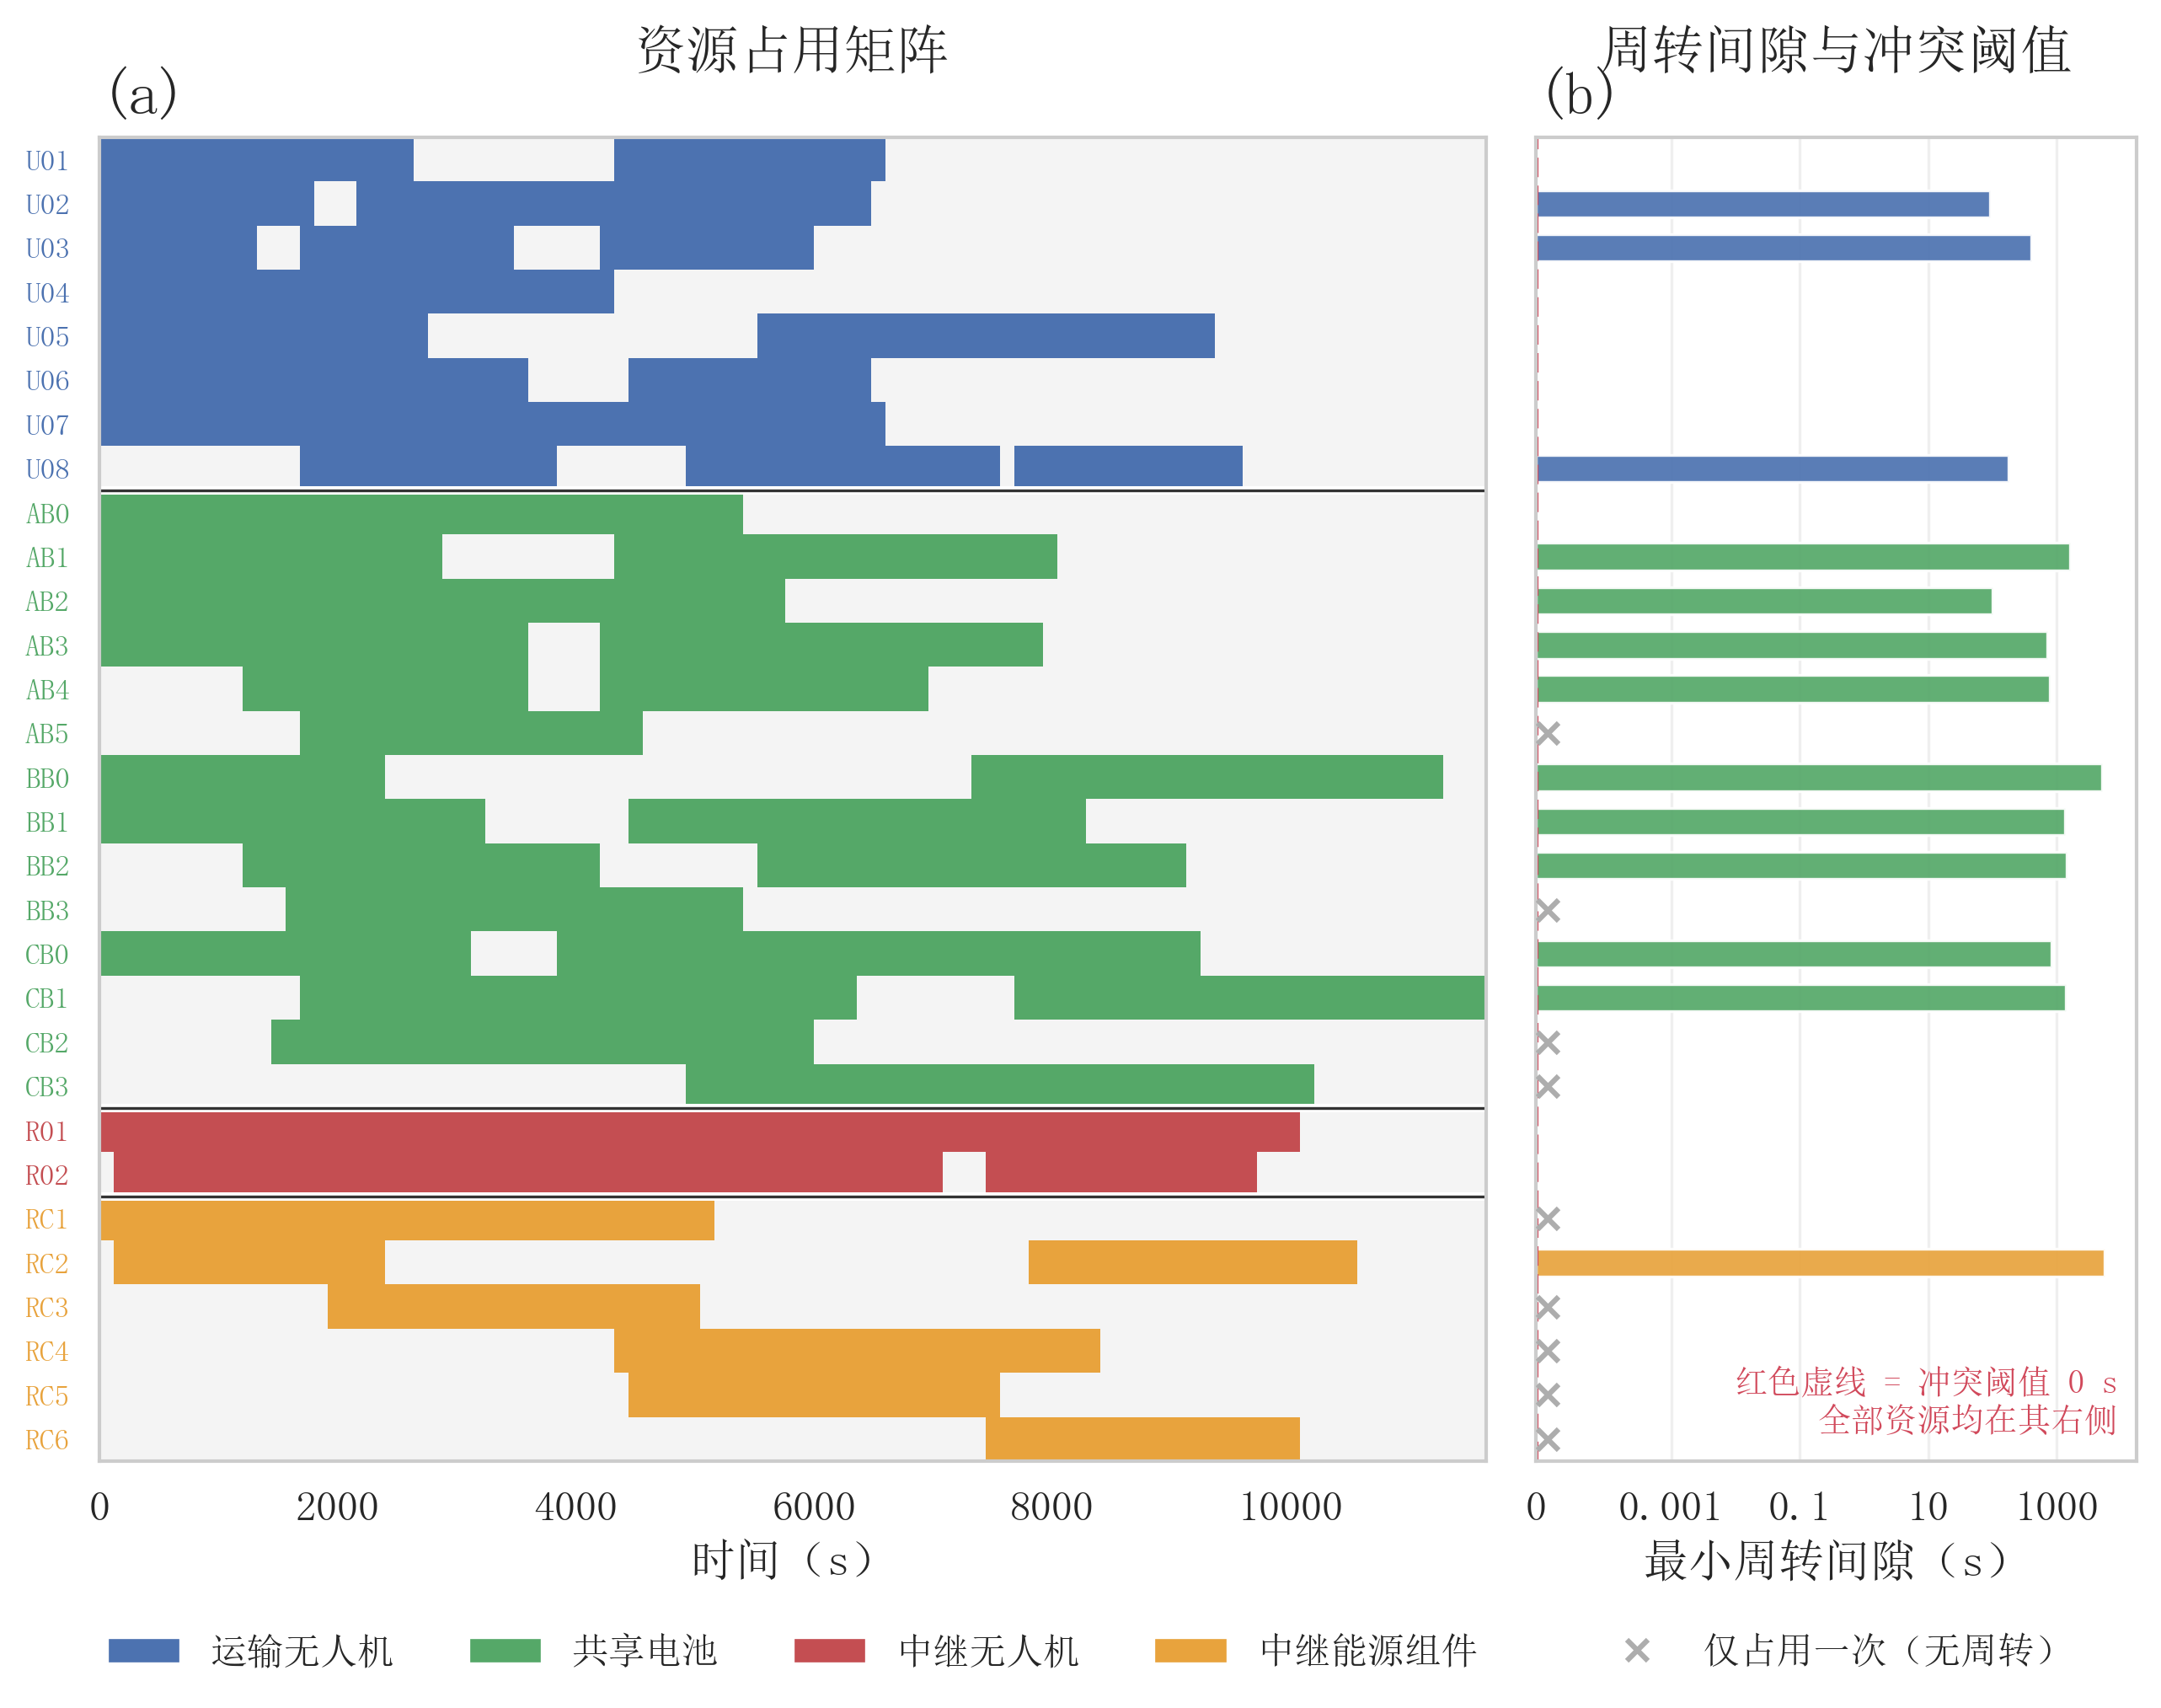
\includegraphics[width=0.95\textwidth]{figures/fig_resource_conflict.png}
	\caption{资源占用矩阵与周转间隙}
	\label{fig:resource-conflict}
\end{figure}

\subsection{灵敏度分析}

返航安全余量 $\rho$ 是影响运输能力的关键参数，其灵敏度已在问题一讨论（图~\ref{fig:q1-sens}）。进一步，表~\ref{tab:sens}归纳了 $\rho$ 对三种机型平均最大安全载荷的定量影响。

\begin{table}[htbp]
	\caption{返航安全余量 $\rho$ 对各机型平均最大安全载荷的灵敏度}
	\label{tab:sens}
	\centering
	\begin{tabular}{cccc}
		\toprule
		$\rho$ & A 型（kg） & B 型（kg） & C 型（kg） \\
		\midrule
		0.10 & 25.00 & 30.00 & 78.68 \\
		0.20 & 25.00 & 29.91 & 75.09 \\
		0.30 & 23.88 & 28.12 & 68.51 \\
		0.40 & 16.67 & 23.17 & 52.64 \\
		\bottomrule
	\end{tabular}
\end{table}

可见 C 型对 $\rho$ 最敏感（$\rho$ 每增大 10\%，平均载荷下降约 8.7\,kg，即由 $\rho=0.10$ 时的 78.68\,kg 降至 $\rho=0.40$ 时的 52.64\,kg），A、B 型相对稳健。这表明在应急场景下若需提高返航安全余量，重载机型的有效运力将明显下降，须相应增加架次或改用更小型号，体现了安全性—运输效率的权衡。

单因素扫描固定了电池可用能量不变，无法反映参数间的耦合。考虑到山区低温会同时压低电池
可用容量，本文进一步引入电池可用能量折减系数 $\kappa$（即 $E_g^{\mathrm{use}}\to\kappa E_g^{\mathrm{use}}$），
与 $\rho$ 构成二维扰动网格，如图~\ref{fig:q1-sens2d}所示。

\begin{figure}[htbp]
	\centering
	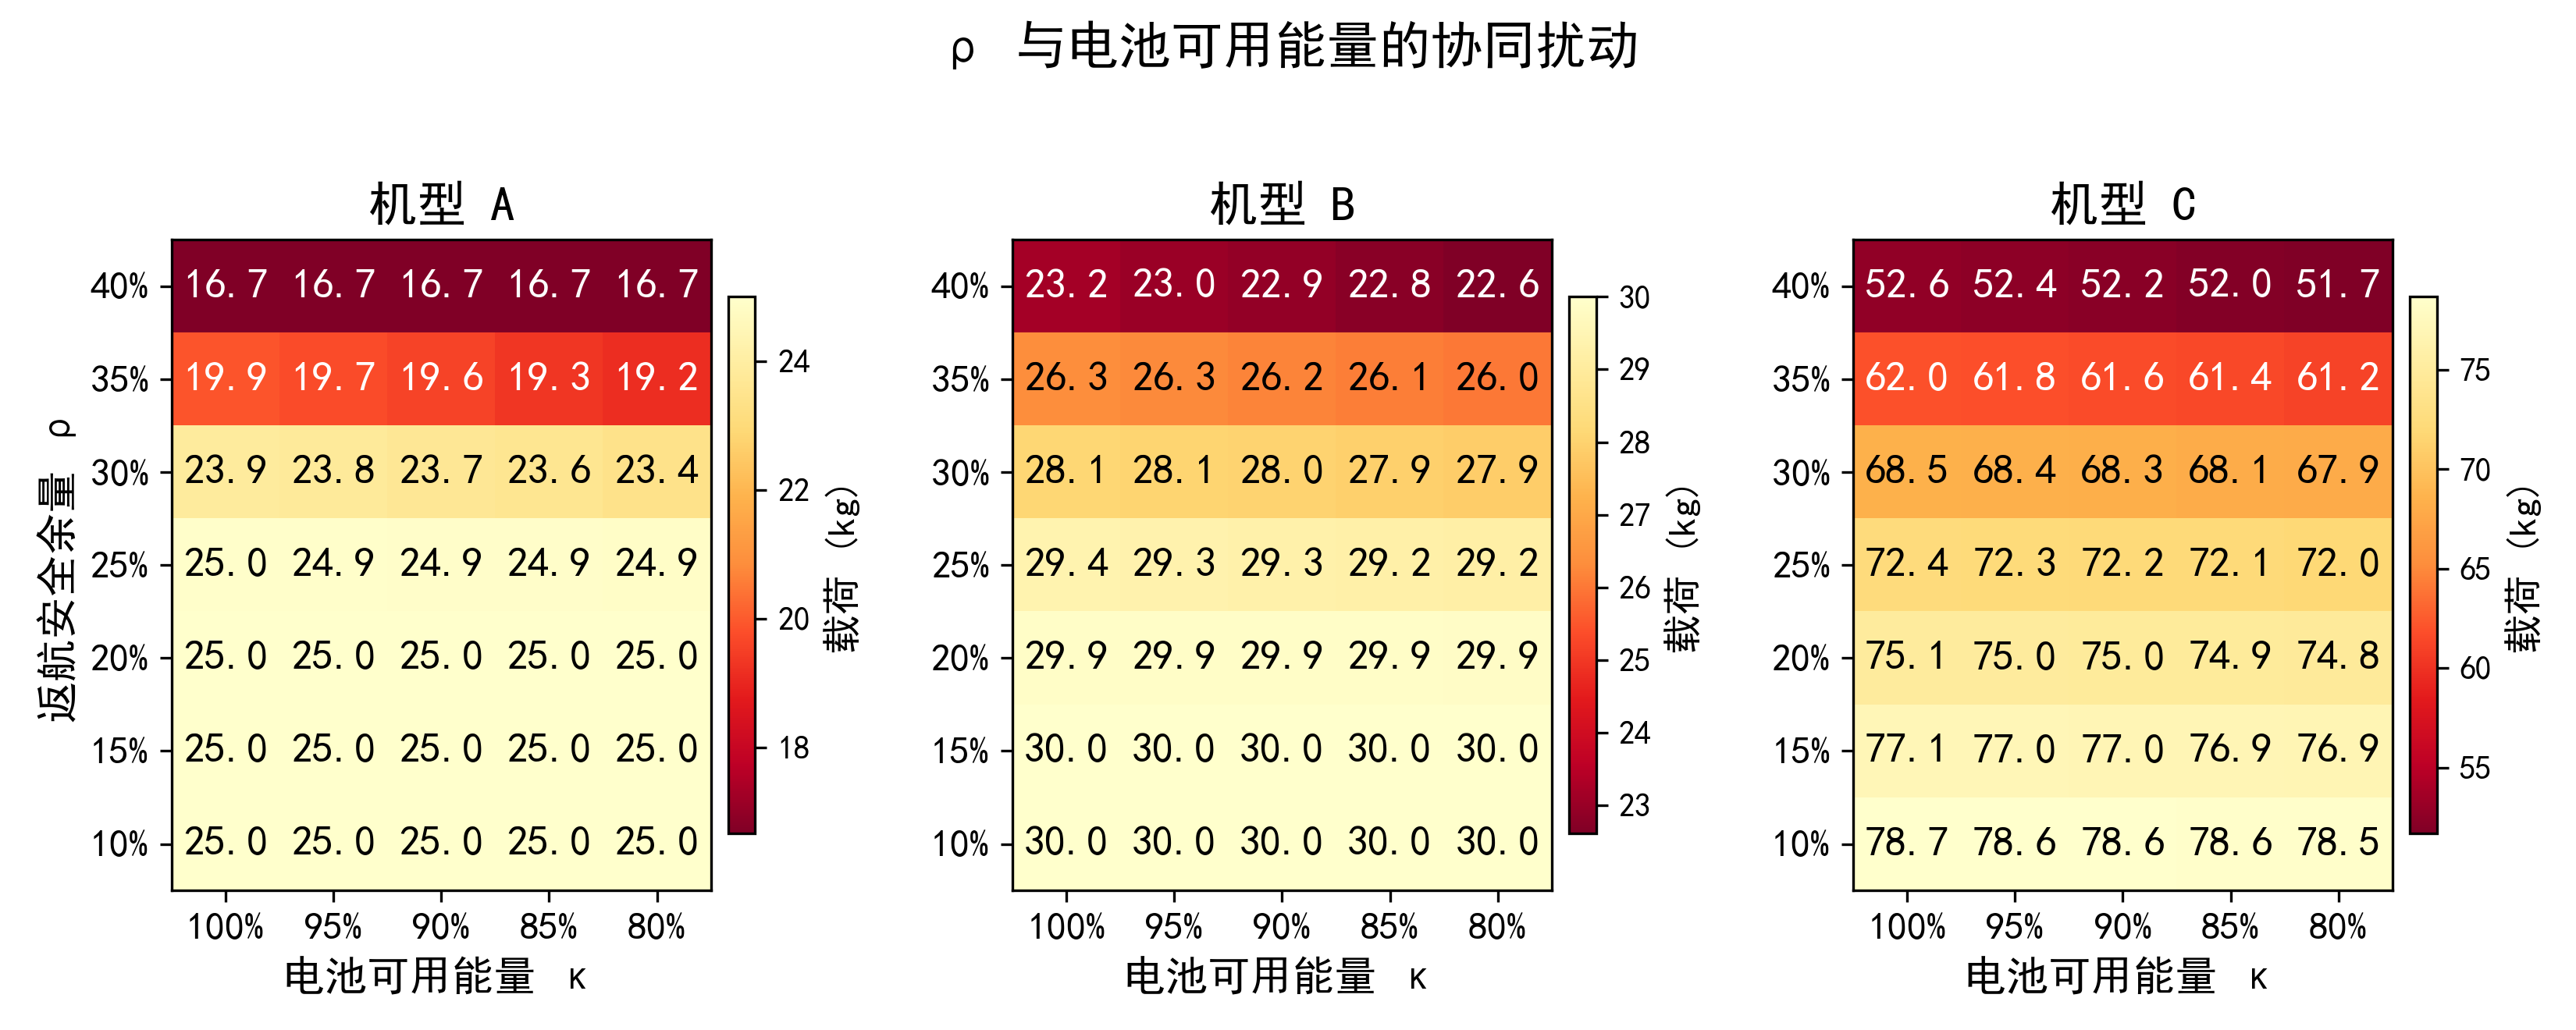
\includegraphics[width=0.95\textwidth]{figures/fig_q1_sens2d.png}
	\caption{返航安全余量与电池可用能量的协同扰动}
	\label{fig:q1-sens2d}
\end{figure}

以 $\rho=0.10$、$\kappa=1.00$ 为基准，A、B、C 三型“仅 $\rho$ 升至 0.40”的降幅分别为
8.33、6.83、26.04\,kg，“仅 $\kappa$ 降至 0.80”的降幅分别为 0.00、0.00、0.18\,kg，
而两者同时发生的实际降幅为 8.33、7.38、26.99\,kg，与两项降幅之和的比值为
1.000、0.925、0.971，均在 1 附近。这说明\textbf{在这三个两项同时劣化的算例上未见耦合放大}，
两因素的不利影响基本可加：配置运力时应按最坏组合留裕度，而不能指望一项劣化被另一项抵消。
必须限定这一点：三个角点算例不足以支撑“参数空间内不存在耦合放大”这样的全称结论——
真正的判据是显式的交互项及其在全部“服务区$\times$机型$\times$参数网格”上的符号，
而这需要全因子扫描，本文未做。因此本节只报告“未见放大”，不报告“不存在放大”。
图中还可读出各机型的失效边界：$\rho=0.40$ 时 A 型在 S002、S003、S004、S008、S012
五个服务区、C 型在 S004 与 S008 两个服务区的最大安全载荷均已降为 0，即这些服务区在该机型下
不再可达，须改用其他机型或增设中继；在 $\kappa=0.80$、$\rho=0.40$ 的最坏组合下，
C 型平均载荷进一步降至 51.69\,kg。A、B 两型在 $\rho=0.10$ 时对 $\kappa$ 降至 0.80
完全不敏感（降幅 0.00\,kg），说明其运力瓶颈是额定载质量而非能量；
C 型在同组合下也仅降 0.18\,kg，其受 $\kappa$ 的压制要到更高 $\rho$ 才明显。

\subsection{结果交叉验证}

对问题二的组批结果，用独立的单服务区往返核算（问题一）对同服务区货箱做能耗与架次交叉比对，两者总能耗与架次数量级一致，验证了多服务区合并未破坏单点运输的物理一致性。对问题三的中继方案，独立复核不采信结果表记录的悬停离地高度，而是取表内经纬度回原始 DEM 重新求地面高程再相减；能源组件的周转时刻由“返回时刻＋充电时长”从能耗列反算，与求解器的内部状态无关；并逐段核对标为“中继”的时段确实落在某个中继架次的服务窗口内、标为“中断”的时段不挂架次编号。对问题四，最优分区由完全枚举给出，并用组列集合划分整数规划走第二条路径复核，两条路径给出相同的最优资源规模（$K=2$ 为 31、$K=3$ 为 34）。

此外，问题二的启发式解另有两层小规模精确验证：分区层在 3 服务区算例上与列生成＋集合划分整数规划的最优解间隙全部为 0；时序层用 big-$M$ 析取规划给出「给定贪心指派，贪心调度已近最优」的证书（最短完工口径差 $2.40\%$、加权时延口径差 $5.75\%$）。两层的适用范围已在 6.4 节如实界定，此处不再重复。

上述交叉验证都在数值层面进行，图~\ref{fig:solution-network}则从\textbf{结构层面}给出同一结论。该图把推荐方案还原为「服务区（15）$\to$运输架次（24）$\to$机型／悬停站」的多层网络，全部连边由独立脚本重新读取 \texttt{q3\_\allowbreak transport\_\allowbreak trips.csv}（问题三错峰后的最终运输方案）、\texttt{q3\_\allowbreak comm\_\allowbreak phases.csv} 与 \texttt{q3\_\allowbreak relay\_\allowbreak trips.csv} 建立，不引用求解器的任何中间状态。架次列按机型分组排列，故右侧「架次$\to$机型」成为三段互不交叉的平行束，可一眼读出 A 型 11 架次、B 型 7 架次、C 型 6 架次；左侧每个架次的连边数即其访问的服务区数，24 个架次共 27 条访问边，其中 3 个架次跨两个及以上服务区，正是问题四绑定原子任务单元的来源。虚线给出中继保障关系，19 条边中 6 条落在 S05、5 条落在 S01、4 条落在 S03、3 条落在 S02、1 条落在 S04，与表~\ref{tab:q3-stations}中五站分别保障 6、5、4、3、1 个区间的分布相互印证。

这张图同时是\textbf{接口一致性的图示证据}：层与层之间的对应关系完全由结果表决定，问题二若改动机型指派、或问题三若改变架次与悬停站的绑定，图的连通结构会立刻随之改变，不可能在未被察觉的情况下与另两问脱节。

\begin{figure}[htbp]
	\centering
	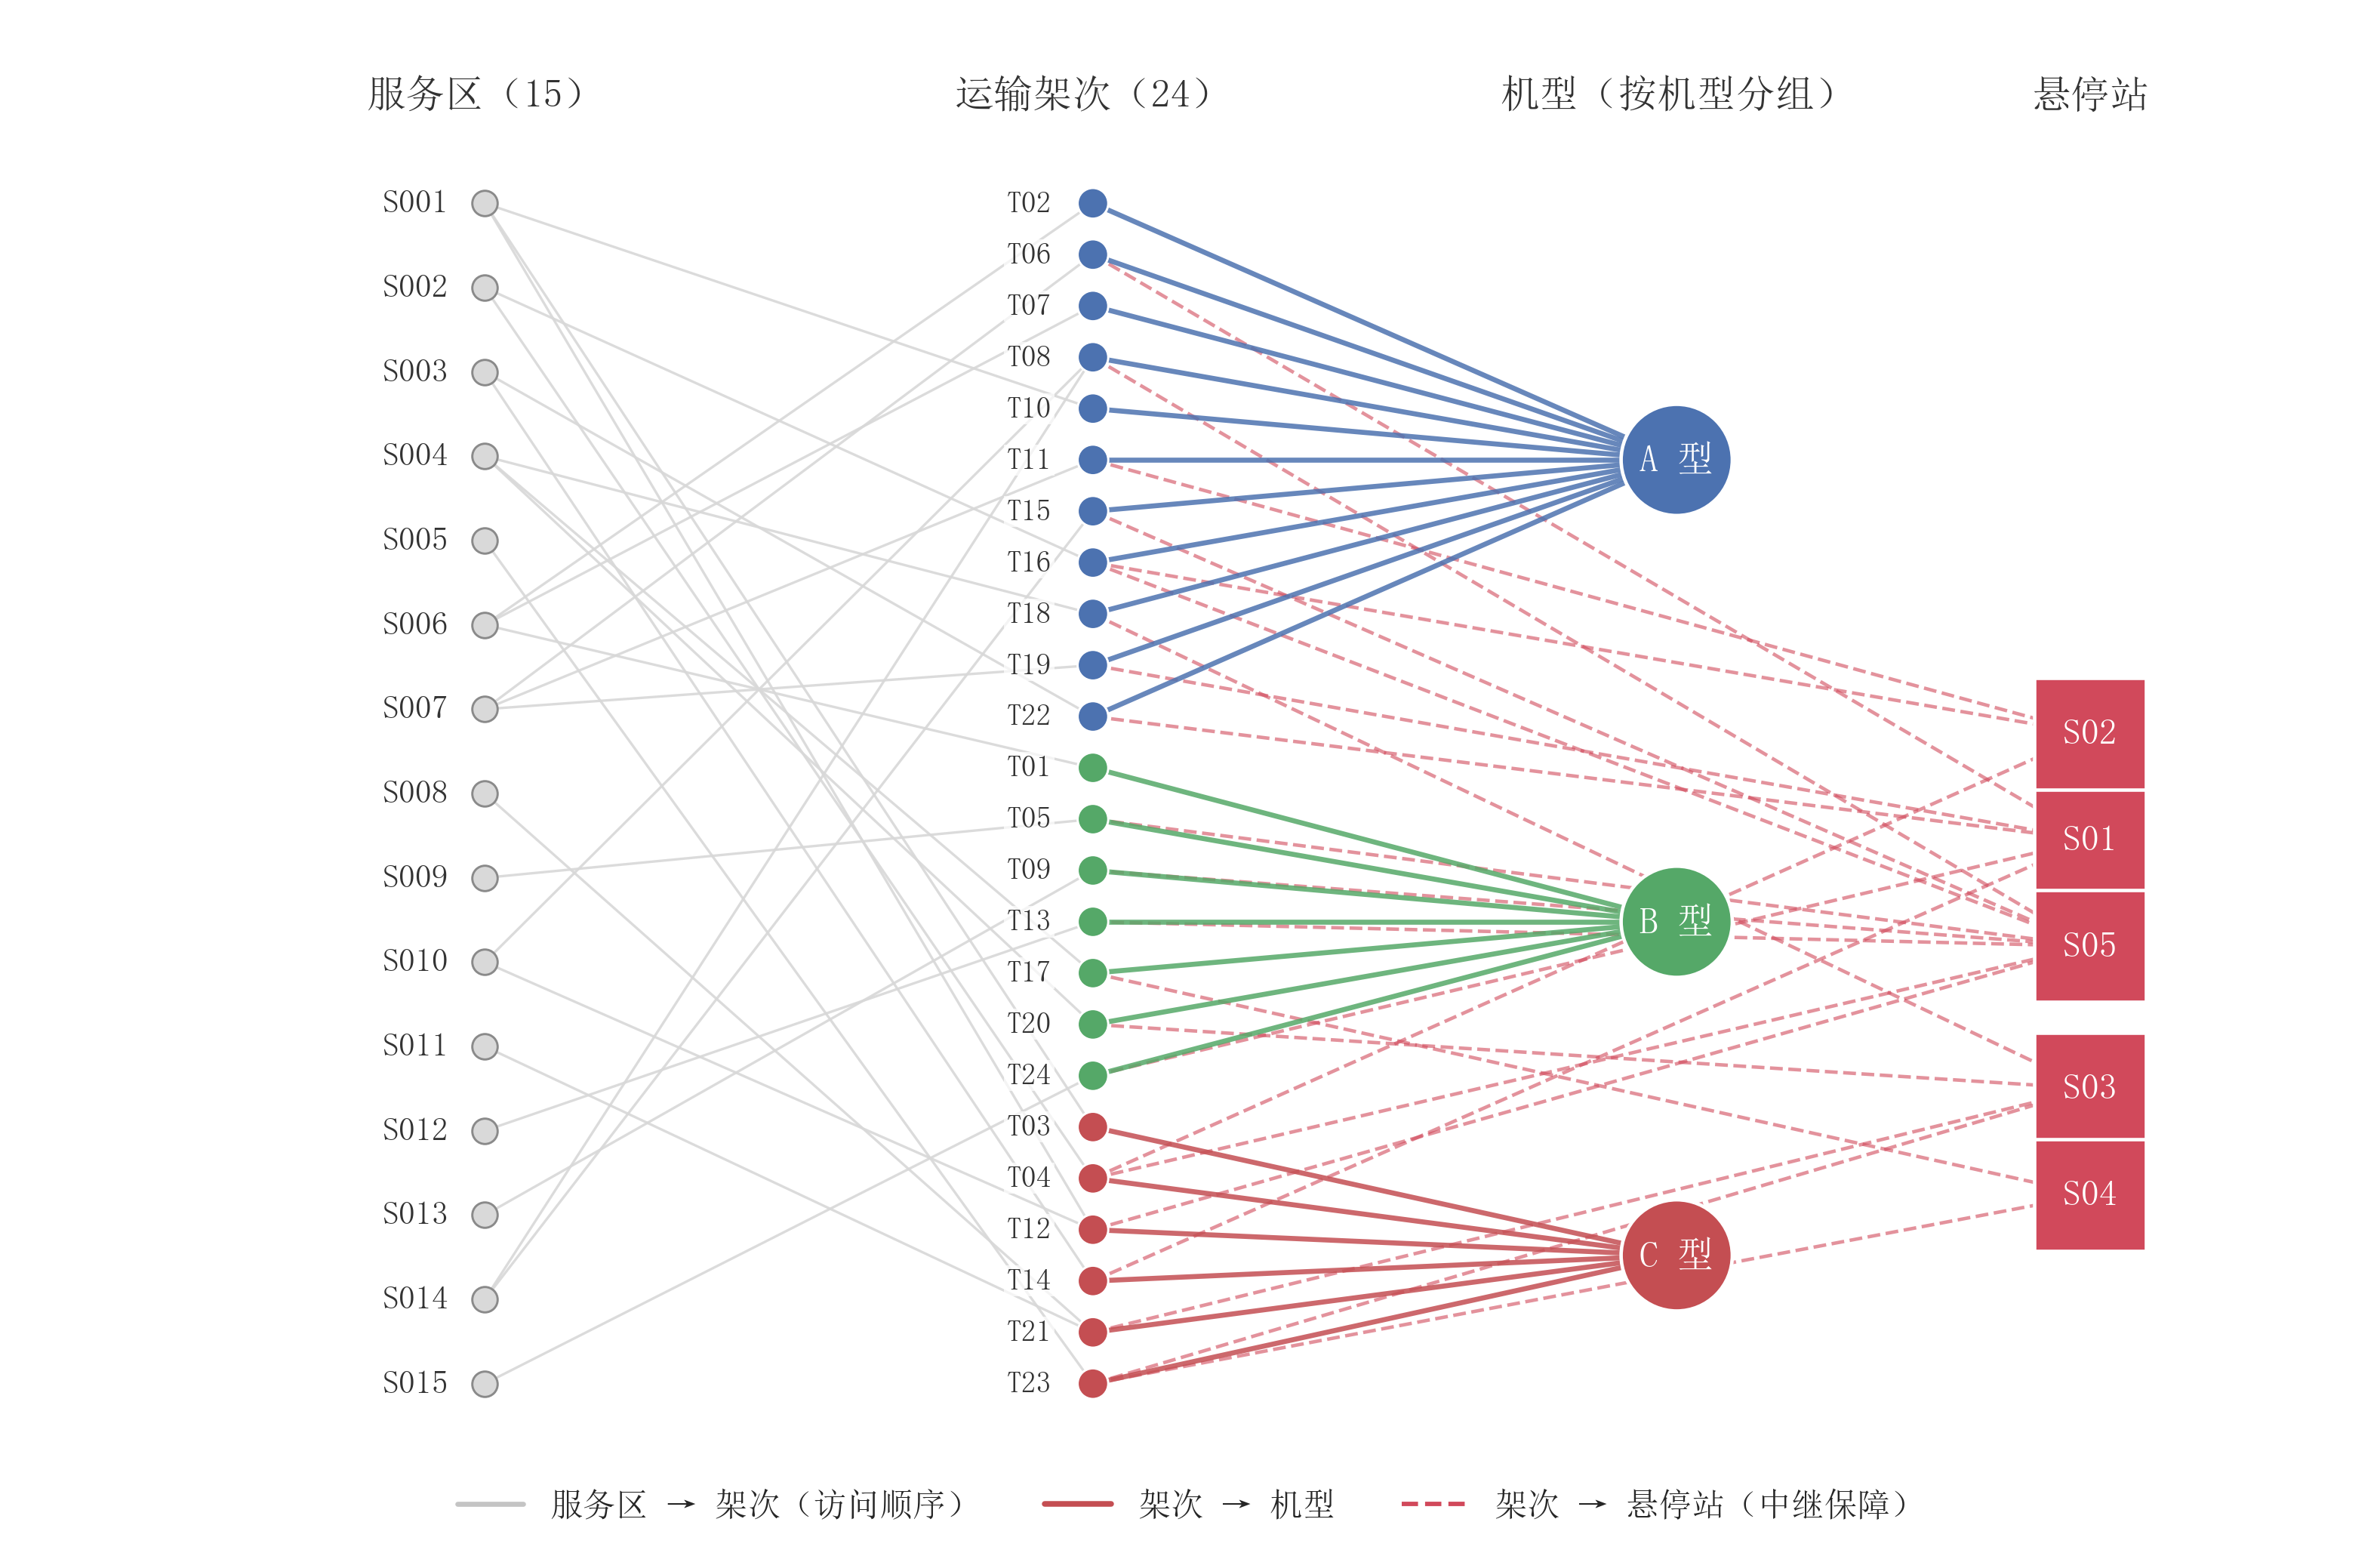
\includegraphics[width=0.95\textwidth]{figures/fig_solution_network.png}
	\caption{服务区—架次—机型—悬停站网络}
	\label{fig:solution-network}
\end{figure}

\subsection{DEM 口径与离散化误差}
\label{sec:dem-caliber}

地形净空是全部四个问题的公共输入。这里把\textbf{计算口径}（算的是哪个量）与
\textbf{离散化误差}（同一个量算得准不准）分开检验——前者是定义问题，后者是精度问题，
不能用后者的检验替代前者。

\textbf{巡航高度的口径。}题面附录 2 规定计划巡航海拔取“该航段所经过 DEM 像元的最高
地面高程以上 50\,m”，即式~\eqref{eq:cruise-alt} 中的
$\mathcal{C}(\overline{ij})$ 是航段\textbf{穿过}的 30\,m 像元集合，
$z_{\mathrm{DEM}}$ 取像元的\textbf{原始}高程。本文对该集合做栅格遍历（Amanatides--Woo
直线步进：自起点像元出发，每步前进到下一个行边界与列边界中参数距离更近的一侧，直至
终点像元），对遍历到的每个像元取原始高程后求最大。

\textbf{一个已更正的错误口径。}本文早期版本曾把这一步实现为“沿航段按固定步长采样、
对双线性插值面取最大”。这是\textbf{算错了量}：插值值是像元四角高程的凸组合，其沿线
最大值结构性地不高于所经过像元的原始最大值，会把巡航高度系统性压低。以 120 条节点
航段实测，两种口径的差异为：\textbf{76\% 的航段被低估}，最大低估 16.17\,m
（S006$\to$S008），均值 2.65\,m、中位 1.72\,m，$|\Delta|\ge5$\,m 的 31 条、
$\ge10$\,m 的 12 条；同时另有 29 条被\textbf{高估}最多 10.72\,m——航线贴近像元边缘时，
插值把航线并未进入的邻元高程混了进来。可见该口径在两个方向上都有偏。

偏差方向必须说清楚：低估 $H_{\max}$ $\Rightarrow$ 低估巡航海拔 $\Rightarrow$ 低估爬升量、
飞行时间与能耗，属\textbf{非保守}误差，会造成“按模型算飞得到、实际能量不够”的风险。
这与“低估地形所以偏保守、更安全”的直觉恰恰相反，也与本文早期版本中的表述相反，
此处一并更正。

\textbf{栅格遍历的正确性。}遍历是否漏掉航段真正穿过的像元，是本环节唯一的危险方向
（漏即低估）。以 0.5\,m 超密采样所得的像元集合为参照，对全部 120 条航段核对：
\textbf{漏像元 0 个}，因漏像元导致的高程低估 0.000\,m；另有 119 个像元仅出现在遍历
结果中，是航线擦角而过、遍历计入的格子，方向保守。

\textbf{口径修正的方案层影响。}航段层最大为单段 $+14.55$\,s、$+4.3\times10^{-3}$\,kWh；
折算到方案层，问题一推荐方案总能耗 $+0.029\%$、总作业时间 $+0.143\%$，45 个
“服务区$\times$机型”组合中仅 6 个的最大安全载荷发生变化，幅度
$-0.168\sim+0.026$\,kg。即本次修正不改变任何服务区的可达性判定与架次划分。
量级虽小，但它是物理量定义层面的更正，量级小并不构成不修的理由。

\textbf{视线遮挡判定的采样步长。}口径更正后，采样步长（$5$\,m）只剩视线遮挡判定
一个用途，故此处要问的不是“最高地形被低估多少”，而是“步长会不会把遮挡判反”。
对 120 条节点连线分别在 5\,m 与 1\,m 步长下判定，结论\textbf{翻转 0 条}；沿线净空
余量最小 39.2\,m、中位 51.5\,m，没有任何一条连线贴近遮挡阈值（$<1$\,m 者 0 条）。
说明 5\,m 步长对遮挡判定有充分裕度，且判定结果对步长取值不敏感。

\textbf{插值方式（仅用于遮挡判定）。}遮挡判定沿连线做双线性插值采样。设像元四角
高程为 $v_{00},v_{01},v_{10},v_{11}$，插值结果为 $z(\xi,\eta)=\sum w_{ij}v_{ij}$，
权系数非负且和为 1，故 $\min v_{ij}\le z\le\max v_{ij}$：插值面恒被四角高程夹住，
不会产生超出局部真实地形的虚假尖峰而把连线误判为遮挡，且在像元边界上连续。对
20000 个随机探针实测，越出所在像元四角高程区间的个数为 0。

需要界定这一结论的适用范围：它\textbf{只}支持“插值用于遮挡判定是安全的”，
\textbf{不能}用来论证巡航高度口径正确。要注意“被四角夹住”里的四角是该采样点
\textbf{所在像元}的四角，与遍历口径计入的像元集\textbf{并不是同一个集合}——航线
贴角而过时，插值会混入遍历未计入的邻元。因此插值面的沿线最大值\emph{相对遍历
口径的最大值而言并不必然更小}：本数据上多数航段（76\%）偏低，但偏差是双向的，
另有 29 条高估最多 10.72\,m（9.4 节已如实报告）。把一个有条件的局部性质同时
当作“此处可用”的依据和“彼处正确”的论据，是本文早期版本在这一节上的实质疏漏。
       % 九、模型检验与分析
\section{模型的评价与推广}

\subsection{模型的优点}

\begin{itemize}
	\item \textbf{物理口径统一、可复现：}四个问题共享同一套地形净空、等效航程、能耗、充电与通信链路模型，单位、对象编号与计算口径一致，全部计算可由独立 Python 脚本复现，数据与结论可追溯。
	\item \textbf{充分刻画地形与通信约束：}巡航海拔由航段所经过的 DEM 像元最高高程确定，通信状态同时考虑视线遮挡与双向链路预算，较真实地反映了山区环境对运输与通信的双重制约；通信连续性还被写成必须归零的硬指标而非加权项，与题面把「连续通信」列为约束的表述一致。
	\item \textbf{方法选择与问题结构匹配，并以精确解为标尺：}问题一用同质类多重集动态规划在\textbf{允许混用机型}的可行域上求全局最优，并经指派式、集合划分与混用机型三条独立整数规划路径逐行复核（$45/45$、$44/44$，以及 $15$ 区中 $14$ 区一致、S001 因列数超时限如实记为未证最优）；问题二用大邻域自适应搜索（ALNS）配 $\varepsilon$-约束扫描，再用两层小规模精确解标定最优性间隙；问题三用集合覆盖整数规划把悬停高度升为决策变量，并让运输开始时刻进入同一优化问题；问题四用受限增长串完全枚举，枚举结果即全局最优，另以组列集合划分整数规划复核。四问的计算量均在合理时间内完成。
	\item \textbf{揭示多目标权衡：}通过架次数上限—能耗—完成时间的非支配前沿、返航余量—电池能量的二维扰动、通信中断归零的完成时刻代价、以及分区组数—资源规模—均衡度三组定量对照，量化了及时性—能耗—架次、安全性—运力、通信连续性—任务时长、均衡—资源之间的权衡关系，为决策提供了方向性依据。
\end{itemize}

\subsection{模型的缺点}

本文如实列出尚未消除的残留问题，不以「已用高级算法」掩盖其局限。

\begin{itemize}
	\item \textbf{启发式的全局最优性未经证明：}问题二的 ALNS 仍是启发式算法。虽然两层小规模精确验证给出了 Layer A 三个算例间隙全为 $0$、Layer B1/B1$'$ 的最优性证书，但这些算例只含 3 个服务区、8 架无人机对至多 9 个架次，\textbf{机队资源竞争几乎不存在}，故它验证的是组批、能耗、路径与时序逻辑的正确性，\textbf{不能}外推为「全局资源拥塞情形下已证最优」。
	\item \textbf{自由指派层的整数规划间隙很大：}Layer B2 放开了无人机与共享电池的物理指派，求解 90\,s 后最优性间隙仍有 $63.55\%$，只能作为搜索方向上的佐证，\textbf{不构成最优性证明}；同层 B1 的最优解虽已证最优，但该解本身违反 8 项硬时限，故只作下界参考而不作为可行方案。
	\item \textbf{消融实验暴露了一处搜索质量问题：}ALNS 全量配置 ④ 的可行解集严格包含配置 ③，其完成时间（$8041.7$\,s）却比 ③（$7188.7$\,s）劣 $11.9\%$。原因是加权时延归零后目标面变得平坦，而 ④ 的解空间更大，固定迭代预算下更容易停在局部解。本文在 6.4 节如实报告该现象，未将其粉饰为「全量搜索更优」。
	\item \textbf{换站修复产生的新悬停站未经连续精化：}问题三的第三级修复动作为了让某区间「改换一个届时真正在位」的悬停站，会从候选表中直接取站，该站\textbf{未经过} \texttt{refine\_station} 的 $({\rm lon},{\rm lat},h)$ 坐标下降精化。精化会改变站址、进而改变去程时长与建链时刻，因此不能在排班完成后再补做。这些站的有效性由覆盖矩阵的全密度复核保证，但接入裕量不如精化过的站；最终方案一律以 $\Delta t=1$\,s 的逐时刻审计为准。
	\item \textbf{分区方案在给定库存下均不可行，且分区本身在放大资源需求：}问题四的结论是 $K=2$ 与 $K=3$ 在现有库存下都不可行（63 / 301 个分区中库存可行分区数均为 0）。这不是搜索不足，而是题面「各类资源不得跨组调配」这一规则的直接后果——每组必须自备中继护航，使中继无人机需求至少为组数 $K$，而主力组自身峰值就需 2 架。也就是说，\textbf{分区在放大中继与 B 型机队的需求}，本文只能给出补配清单而非可行分区。
	\item \textbf{部分参数为简化假设：}未考虑风场、雨雾、起降排队、充电桩数量等实际因素对飞行与周转的影响。
\end{itemize}

\subsection{模型的改进}

\begin{itemize}
	\item 对问题二可延长迭代预算或采用多起点并行搜索，以缓解上述 ④ 的搜索质量问题；对 Layer B2 可加入割平面或列生成以缩小 $63.55\%$ 的间隙，把自由指派层的最优性也纳入验证范围。
	\item 对问题三可把换站后的新站补做连续精化，但精化必须与排班\textbf{联合迭代}而非事后追加，否则站址变化会使已排定的建链时刻失效。
	\item 对问题四可引入跨组资源共享协议（如资源的时分复用或动态调配许可），以降低「不得跨组调配」带来的机队放大效应；也可在目标中显式加入工作量均衡项，以避免多分组反而更不均衡的现象。
	\item 可建立充电桩数量约束下的多队列充电仿真，细化电池周转模型。
\end{itemize}

\subsection{模型的推广}

本文的“地形感知飞行＋能量余量＋通信链路”联合框架，可推广至其他山区/海岛/灾区的无人机物流、电力巡检、应急通信中继等场景；任务分区与资源配置核算方法也可用于多作战单元、多救援分队的兵力/资源编配决策。
      % 十、模型的评价与推广
\section{结论}
\label{sec:conclusion}

本章把四问的答案汇总到一处。摘要说明本文做了什么，表~\ref{tab:overview} 给出四问各自交付的那一个方案，第~\ref{sec:evaluation} 章评价方法本身的好坏与可推广性；本章回答的是另一个问题——这四问的结论分别是什么、能拿去做什么、在什么条件下成立。本章只汇总第~\ref{sec:validation} 章复核过的结论，不新增计算，也不新增数字。

\subsection{四问的主要结论}

\textbf{问题一给出的是运力边界与最省架次的组批方案。}在允许同一服务区混用机型的可行域上，\mtQoneTrips\ 架次可覆盖全部 80 个货箱，总能耗 \mtQoneEnergy\,kWh、累计作业时间 \mtQoneWorkTimeH\,h；相较限定「一个服务区只用一个机型」时的 $63.180$\,kWh，混用机型在架次数不变的前提下节能 $6.24\%$。该结论另由三条互不相同的精确路径逐行比对，结果一致（表~\ref{tab:q1ilp}）。与之配套的是一条必须一并读的边界：返航安全余量超过 $0.3513$ 后本方案整体失效，而率先失去可达性的\textbf{不是}载重最大的 C 型、而是航程最短的 A 型——$\rho>0.2992$ 时 A 型空载亦无法往返最不利的 S008（5.3 节）。

\textbf{问题二给出的是资源受限下按时交付的 24 架次调度方案。}8 架运输无人机与 14 组共享电池全部投入周转，\mtQtwoRecTrips\ 个架次在 \mtQtwoMakespan\,s 内完成全部 80 个货箱的交付，加权时延与硬时限违约均为 $0$，总能耗 \mtQtwoEnergy\,kWh（表~\ref{tab:hardcheck}）。调度结构本身是效率的一等来源：在组批不变的条件下仅调整派工顺序，完成时间即下降 $31.9\%$。该方案附带一个不应被略过的条件——两层小规模精确验证中 \mtQtwoExactProved\ 例取得了最优性证书、\mtQtwoExactTimeout\ 例超时后如实以上界报告，而这些算例只含 3 个服务区、机队资源竞争几乎不存在，故它们的作用是对齐组批、能耗、路径与时序的逻辑，\textbf{不能}外推为本方案在大规模机队竞争下也已取得最优性证书（6.4 节）。

\textbf{问题三的结论是一条权衡：连续通信的硬约束会把问题二的高效方案判为不可执行，而消除中断要付出完工时刻的代价。}沿问题二的 \mtQtwoRecTrips\ 条三维轨迹逐时刻判定，只有 \mtQthreeDirect\ 的时间可直连、\mtQthreeRelayFrac\ 处于通信盲区（表~\ref{tab:commcheck}）。把运输开始时刻与错峰、悬停站址与离地高度、中继架次调度放进同一优化问题后，\mtQthreeStations\ 个悬停站、\mtQthreeRelays\ 次中继出动（共 \mtQthreeRelayVisits\ 次悬停站服务）以 \mtQthreeRelayEnergy\,kWh 把中断时间占比降至 \mtQthreeGap。代价是联合完工时刻由 \mtQtwoMakespan\,s 推迟到 \mtQthreeJointDone\,s（$+2.1\%$），而迟到箱数与加权迟到仍为 $0$、最小硬时限余量 \mtQthreeMinMarginFine\,s（表~\ref{tab:q3chain}）。还有一条只在本方案成立的观察：六站离地高度落在 $65\sim185$\,m、没有任何一站触及题给的 $300$\,m 上限，中继能量占用比最高仅 $0.740$，说明限制保障能力的是时序结构与站址几何而不是能量——换站址、加大服务窗口或放宽并发都会改变这一占用比，该观察不外推。

\textbf{问题四给出的不是一张时刻表，而是一条关于约束的发现。}按「同一架次访问的服务区不可拆分」把 15 个服务区绑定为 \mtQfourUnits\ 个原子任务单元后，$K=2$ 与 $K=3$ 分别有 \mtQfourPartKTwo\ 与 \mtQfourPartKThree\ 种分区，逐行枚举即得全局最优；按题面「资源不得跨组调配」复核，两类的库存可行分区数均为 \mtQfourFeasible（表~\ref{tab:q4check}），即「资源不得跨组调配」与题给库存在本算例下不相容。枚举进一步厘清了成因：八类资源各自的最小缺口在两 $K$ 下全部为 $0$，单独看任何一类都存在一个不超库存的分区，故不可行来自八类资源无法在同一分区内同时取到各自最小值的\textbf{联合约束}，而不是任何单一类别的短缺（表~\ref{tab:q4-min}）。其中中继无人机离临界最近：每个含失效区间的组都须自备通信保障，故需要中继的组数下界为 $K-1$，$K=3$ 时恰为 $2$、等于库存，余量为 $0$。推荐分区上的缺口是「先省资源、再求均衡」这一目标的代价：$K=2$ 缺 \mtQfourGapSum\ 件、$K=3$ 缺 \mtQfourMinPatchKThree\ 件。

\subsection{可信度与适用边界}

上述结论的可信度来自四条互不相同的复核路径（表~\ref{tab:overview}）：复核脚本\textbf{只读}四问的结果表重算硬约束，不复用求解器的任何中间变量，故它能排除程序内部状态与结果表之间的串号、漏检与自我印证。但该脚本与求解器仍共享公共物理模块，因此它\textbf{不能}排除公共物理模型本身的口径错误——后者只能靠 DEM 口径对照与原始数据判读（第~\ref{sec:dem-caliber} 节）。这条边界不在结论层放宽。

以下五条界定本文结论的适用范围，逐条见第 10.2 节。（1）问题二的推荐方案只在小规模算例上取得了最优性证书，其全局最优性在大规模机队竞争的情形下未被覆盖。（2）放开物理指派后得到的可行上界违反 9 项硬时限，只能作搜索方向上的佐证，其最优性间隙如实报出。（3）遮挡判定是二值的几何视线判据，未含第一菲涅尔区净空、绕射与多径，故直连时间占比应读作偏乐观的上界。（4）全文未建模运输无人机之间的最小安全间隔与高度层分配，冲突只在「同一资源不被两个任务同时占用」的意义上被排除。（5）问题四的否定结论只在本文 \mtQfourUnits\ 个原子单元的划分方式与题给库存下成立，换一种划分须重新核算。

\subsection{面向救援调度的建议}

把四问的结论落到调度决策上，本文给出四条建议，按可落地程度排序。

\textbf{第一，首选不分区、按单组执行。}这是全篇唯一无需任何补配即可交付四问的方案：以问题三的运输—中继联合调度整体执行，其资源需求不超过现有库存（8 架运输无人机与 14 组共享电池全部投入周转，见 6.3 节）。分区虽然便于并行指挥，却在题面「资源不得跨组调配」的规则下不可行。

\textbf{第二，若必须分区，则先补配再分区。}按推荐分区计，$K=2$ 缺 \mtQfourGapSum\ 件、$K=3$ 缺 \mtQfourMinPatchKThree\ 件，类别明细见 8.3 节的缺口表；中继无人机的补配不应按「够用即可」只补到推荐分区的水平，而至少要按下界 $K-1=\mtQfourRelayNeed$ 架预留。补配政策给两个参考阈值：$K=2$ 时把八类资源逐类各加 1 件，即有 \mtQfourThreshKTwoMOne\ 个分区可以落地；$K=3$ 时要逐类各加 2 件，才出现 \mtQfourThreshKThreeMTwo\ 个可落地的分区。

\textbf{第三，提高返航安全余量要付运力代价，且这份代价并不均匀。}$\rho$ 超过 $0.2992$ 先剥夺 A 型对 S008 的可达性，超过 $0.3513$ 则方案整体失效。因此加严安全余量不能单独做，必须与「增加架次或调整机型配比」同时进行，否则会在某个阈值处直接失去对个别服务区的可达性。

\textbf{第四，通信保障的投入方向是时序与站址，而不是能量。}本方案中继能量占用比最高仅 $0.740$，六站高度落在 $65\sim185$\,m、没有一站触及 $300$\,m 的上限，瓶颈在链长与站址几何。这一判断同样带条件：换站址、加大服务窗口或放宽并发都会改变该占用比，届时能量完全可能先触顶，故它只描述本方案。
      % 十一、结论

% === 参考文献 ===
% 按正文首次引用顺序编号；书籍注明引用页码，网络资源注明网址与访问日期，程序注明来源。
\newpage
\phantomsection
\addcontentsline{toc}{section}{参考文献}

% 按正文首次引用次序编号。著录格式依竞赛论文格式规范：
%   书籍      [编号] 作者，书名，出版地：出版社，起止页码，出版年。
%   期刊论文  [编号] 作者，论文名，杂志名，卷期号：起止页码，出版年。
%   网上资源  [编号] 作者，资源标题，网址，访问时间（年月日）。
\begin{thebibliography}{10}
\setlength{\itemsep}{1pt}
\setlength{\parskip}{0pt}

\bibitem{xinhua2026jizhe}
王楚然，杨驰. 记者手记：抵近广西横州镇龙乡，\url{http://www.xinhuanet.com.cn/politics/20260709/acf8e4b353304bb78007d8224f1cd2ef/c.html}，访问时间 2026 年 9 月 20 日.

\bibitem{xinhua2026sanji}
段羡菊，何伟，杨驰，等. 三进“孤岛乡”，\url{http://mrdx.cn/content/20260712/Articel01002NR.htm}，访问时间 2026 年 9 月 20 日.

\bibitem{martello1990knapsack}
Martello S，Toth P. Knapsack Problems: Algorithms and Computer Implementations，Chichester：John Wiley \& Sons，221--245，1990.

\bibitem{dorling2017vehicle}
Dorling K，Heinrichs J，Messier G G，et al. Vehicle Routing Problems for Drone Delivery，IEEE Transactions on Systems, Man, and Cybernetics: Systems，47(1)：70--85，2017.

\bibitem{itu2024p525}
International Telecommunication Union. Recommendation ITU-R P.525-5: Calculation of Free-Space Attenuation，\url{https://www.itu.int/rec/R-REC-P.525-5-202411-I/en}，访问时间 2026 年 9 月 20 日.

\bibitem{zeng2016wireless}
Zeng Y，Zhang R，Lim T J. Wireless Communications with Unmanned Aerial Vehicles: Opportunities and Challenges，IEEE Communications Magazine，54(5)：36--42，2016.

\bibitem{copernicus2024dem}
Copernicus Data Space Ecosystem. Copernicus DEM—Global and European Digital Elevation Model (COP-DEM) Product Handbook（30\,m 分辨率全球数字高程模型），\url{https://dataspace.copernicus.eu/sites/default/files/media/files/2024-06/geo1988-copernicusdem-spe-002_producthandbook_i5.0.pdf}，访问时间 2026 年 9 月 20 日.

\bibitem{zhang2021energy}
Zhang J，Campbell J F，Sweeney D C，et al. Energy Consumption Models for Delivery Drones: A Comparison and Assessment，Transportation Research Part D: Transport and Environment，90：102668，2021.

\bibitem{dji2024m350}
DJI Enterprise. Matrice 350 RTK Specifications（多旋翼无人机技术参数），\url{https://enterprise.dji.com/matrice-350-rtk/specs}，访问时间 2026 年 9 月 20 日.

\bibitem{ti2017charger}
Texas Instruments. Li-Ion Battery Charger Solution Using an MSP430 MCU（Application Report SLAA287B），\url{https://www.ti.com/lit/an/slaa287b/slaa287b.pdf}，访问时间 2026 年 9 月 20 日.

% 以下五条对应第 6、7 章新引入的方法（ALNS、ε-约束、big-M 析取、悬停点选址与集合覆盖），
% 均按 DOI 从 Crossref 权威元数据核验后著录，未补造任何字段。DOI 记在注释里备查：
%   pisinger2007general      10.1016/j.cor.2005.09.012
%   aghaei2011multiobjective 10.1016/j.asoc.2011.02.022
%   grossmann2011generalized 10.1007/978-1-4614-1927-3_4（Crossref 未给卷期，故只著录页码）
%   elnabty2022survey        10.1016/j.phycom.2021.101564（同上，无期号）
%   church1976theoretical    10.1111/j.1538-4632.1976.tb00547.x

\bibitem{pisinger2007general}
Pisinger D，Ropke S. A General Heuristic for Vehicle Routing Problems，Computers \& Operations Research，34(8)：2403--2435，2007.

\bibitem{aghaei2011multiobjective}
Aghaei J，Amjady N，Shayanfar H A. Multi-objective Electricity Market Clearing Considering Dynamic Security by Lexicographic Optimization and Augmented Epsilon Constraint Method，Applied Soft Computing，11(4)：3846--3858，2011.

\bibitem{grossmann2011generalized}
Grossmann I E，Ruiz J P. Generalized Disjunctive Programming: A Framework for Formulation and Alternative Algorithms for MINLP Optimization，The IMA Volumes in Mathematics and its Applications，93--115，2011.

\bibitem{elnabty2022survey}
Elnabty I A，Fahmy Y，Kafafy M. A Survey on UAV Placement Optimization for UAV-assisted Communication in 5G and Beyond Networks，Physical Communication，51：101564，2022.

\bibitem{church1976theoretical}
Church R L，ReVelle C S. Theoretical and Computational Links between the p-Median, Location Set-covering, and the Maximal Covering Location Problem，Geographical Analysis，8(4)：406--415，1976.

\end{thebibliography}


% === 附录 ===
\clearpage
\begin{appendices}
% 往 .toc 写开关：其后的章条目在目录里补上「附录」二字（见 cls 的 \gmcm@toc@appendix）
\addtocontents{toc}{\protect\gmcmtocappendix}
% 附录内图表公式沿用字母编号（附录 A 内为 A.1），与正文的数字编号相区分
\setcounter{table}{0}\setcounter{figure}{0}\setcounter{equation}{0}
\renewcommand{\thetable}{\Alph{section}.\arabic{table}}
\renewcommand{\thefigure}{\Alph{section}.\arabic{figure}}
\renewcommand{\theequation}{\Alph{section}.\arabic{equation}}
\section{求解代码清单}

本文全部求解代码位于项目 \texttt{code/} 目录，每个问题一个独立脚本，按序运行即可复现全文结果。所有代码均为 Python 3 实现，依赖标准科学计算与绘图库（numpy、pandas、matplotlib、seaborn、networkx，以及用于整数规划与二分求解的 scipy），不含随机种子依赖，重复运行结果完全一致。

% 按《人工智能工具及输出使用规定》第 5 条，使用人工智能工具辅助编程的，应在程序前添加
% 注释说明工具名称、版本/型号、开发机构与版本发布日期；各 .py 文件首部均已按要求标注。
% 附录内的表号需与「附录 A」的字母编号一致，这里改用不浮动表格，避免跨节漂移。
\begin{center}
\begin{minipage}{\textwidth}
	\captionof{table}{求解代码与结果文件清单}
	\label{tab:code-list}
	\centering
	\begin{tabularx}{0.98\textwidth}{lX}
		\toprule
		文件 & 说明 \\
		\midrule
		code/core.py & 公共物理模型：数据加载、DEM 采样与遮挡判定、航段时间/能耗/航程、充电模型、通信链路模型 \\
		code/q1.py & 问题一：最大安全载荷二分求解、同质类多重集动态规划组批、指派式与集合划分整数规划双路径复核、$\rho$--$\kappa$ 二维灵敏度 \\
		code/q2.py & 问题二：硬时限约束下的架次构造与共享电池离散事件调度、ALNS 破坏--修复搜索、$\varepsilon$-约束扫描、消融实验与记忆化 \\
		code/q2\_exact.py & 问题二的两层小规模精确验证：列生成＋集合划分整数规划（分区层）、big-$M$ 析取混合整数规划（时序层） \\
		code/q3.py & 问题三：轨迹采样与直连失效区间提取、三维悬停站集合覆盖整数规划、运输错峰与中继架次调度的联合优化 \\
		code/q4.py & 问题四：原子任务单元并查集归并、受限增长串完全枚举、组列集合划分整数规划复核、分组峰值资源需求与缺口核算 \\
		code/verify.py & 独立复核脚本：只读结果表重算第 9 章的全部硬约束、通信连续性与 DEM 离散化误差 \\
		code/fill\_results.py & 把 \texttt{results/*.csv} 回填进《结果提交模板》生成上传用结果表 \\
		code/figures.py & 数据类配图生成脚本（地形图、灵敏度图、直连失效区分布图） \\
		code/figures\_adv.py & 多面板高级配图脚本（帕累托前沿、ALNS 诊断、通信状态时序带、资源雷达图等） \\
		code/make\_roadmap.py & 生成总技术路线图的 .drawio 源文件（版式与图内数值的来源） \\
		code/render\_drawio.py & 把 figures/ 下的 .drawio 示意图离线渲染为 PNG/PDF \\
		results/*.csv & 各问题结果表（对应结果提交模板各 sheet） \\
		figures/*.drawio & 示意图的可编辑源文件（总技术路线图、问题二算法流程） \\
		figures/*.png & 论文插图 \\
		\bottomrule
	\end{tabularx}
\end{minipage}
\end{center}

\section{主要结果数据}

% 依《人工智能工具及输出使用规定》第 4 条，在数据分析结果处加注工具信息。
% 两段都含长串不可断的文件名与英文模型名，必须一起放进 sloppypar，
% 否则 TeX 无法找到合法断点，会产生 Overfull \hbox。
\begin{sloppypar}
\noindent\textbf{数据来源注释：}本文全部数据分析结果由本队在人工智能工具辅助下编写的求解脚本计算得到，所用工具为 DeepSeek，版本/型号 DeepSeek V4.1 Flash（API 模型名 \texttt{deepseek-flash}），版本发布日期 2026 年 9 月 10 日，开发机构为杭州深度求索人工智能基础技术研究有限公司；各脚本首部与支撑材料《AI 工具使用详情》中已列明工具信息与使用过程。全部数据均由本队独立重复运行核验。

问题一最大安全载荷、推荐组批方案、帕累托前沿与双路径复核结果见 \texttt{results/q1\_max\_payload.csv}、\texttt{q1\_recommended\_batching.csv}、\texttt{q1\_pareto.csv}、\texttt{q1\_ilp\_gap.csv} 与 \texttt{q1\_sensitivity.csv}；问题二运输架次、逐箱交付时刻、推荐方案快照、非支配前沿、消融与精确验证结果见 \texttt{results/q2\_transport\_trips.csv}、\texttt{q2\_box\_delivery.csv}、\texttt{q2\_recommended.json}、\texttt{q2\_pareto.csv}、\texttt{q2\_ablation.csv} 与 \texttt{q2\_exact.csv}；问题三悬停站选址、失效区间绑定、中继架次、错峰量、通信阶段与三种口径的覆盖率对照见 \texttt{results/q3\_stations.csv}、\texttt{q3\_intervals.csv}、\texttt{q3\_relay\_trips.csv}、\texttt{q3\_stagger.csv}、\texttt{q3\_comm\_phases.csv} 与 \texttt{q3\_coverage.csv}；问题四原子任务单元、分区配置、全部分区枚举与两类方案对照见 \texttt{results/q4\_units.csv}、\texttt{q4\_partition.csv}、\texttt{q4\_all\_partitions.csv} 与 \texttt{q4\_comparison.csv}。
\end{sloppypar}

\end{appendices}

\end{document}
